%% Select the dissertation mode on
% See the documentation for more information about the available class options
% If you give option 'draft' or 'draft*', the draft mode is set on
%\documentclass[dissertation,final,nocontribution]{aaltoseries}

\documentclass[dissertation,draft*]{aaltoseries} %draft*->final
%\documentclass[dissertation]{aaltoseries}
\usepackage[utf8]{inputenc}

% Set the document languages
\usepackage[english]{babel}        % British hyphenation patterns

%\usepackage[ELEC, RGB]{aaltologo}

\usepackage[babel=true]{microtype} % http://ctan.org/tex-archive/macros/latex/contrib/microtype

\usepackage{graphicx}
 \graphicspath{{graphs/}}
 \DeclareGraphicsExtensions{.pdf}
 
\usepackage{amsmath}% http://ctan.org/pkg/amsmath
%%,amsfonts,amsthm,amsxtra,amsbsy,amssymb,mathrsfs}   % Mathematics
%\usepackage{bm} % bold math argument, http://www.ctan.org/pkg/bm

\usepackage{url}                   % http://ctan.org/tex-archive/macros/latex/contrib/url
\usepackage[caption=false,font=footnotesize]{subfig}                % http://ctan.org/tex-archive/macros/latex/contrib/subfig
\usepackage[labelfont=bf]{caption}
\usepackage{acronym}               % http://ctan.org/tex-archive/macros/latex/contrib/acronym
\usepackage{booktabs}              % http://ctan.org/tex-archive/macros/latex/contrib/booktabs
\usepackage{bytefield}             % http://ctan.org/tex-archive/macros/latex/contrib/bytefield
\usepackage{listings}              % http://ctan.org/tex-archive/macros/latex/contrib/listings
\usepackage{float}                 % Needed for hyperref - see note above
\usepackage{hyperref}              % Problematic - see note above
\usepackage{algorithm}             % http://ctan.org/tex-archive/macros/latex/contrib/algorithms
\usepackage{algorithmic}           % (also part of the algorithms bundle)

\usepackage{longtable}		% for tables that span across pages

\usepackage[footnote,draft,silent,nomargin]{fixme} %added FIXME!

%\floatstyle{plain}
%\newfloat{program}{thp}{figures}[chapter]
%\floatname{program}{Program}

\usepackage{chngcntr}
\counterwithout{footnote}{chapter}


\hyphenation{tele-presence}
\hyphenation{multi-media}

\hypersetup{
  pdfauthor={Varun Singh},
  pdftitle={Enabling Adaptive Multimedia Applications}
  pdfsubject={RTP Congestion Control},
  pdfkeywords={RTP} {Congestion Control} {MPRTP} {geo-location} {Multipath RTP} {Interactive Multimedia}
}



% The author of the dissertation
\author{Varun Singh}
% The title of the thesis: Algorithms and Protocol extensions for Enabling Adaptive Multimedia Applications
\title{Enabling Adaptive Multimedia Applications}

\begin{document}

%% The abstract of the dissertation in English
% Use this command!
\draftabstract{
TBD
}
% Let's add another one in Finnish
%\draftabstract[finnish]{\lipsum[4-6]}
% And yet another one in Swedish
%\draftabstract[swedish]{\lipsum[7-9]}

%% Preface
% If you write this somewhere else than in Helsinki, use the optional location.
\begin{preface}[Espoo]

This dissertation is based on several years of research at Aalto University
(erstwhile Helsinki University of Technology) and standardization at the 
Internet Engineering Task Force (IETF).

\end{preface}

%% Table of contents of the dissertation
\tableofcontents

% For article dissertations, remove if you write a monograph dissertation.
\publicationdataorder{author}{title}{publication}{information}{month}{year and page}
\publicationpunctuation[]{,}{}{,}{,}{,}{}
\publicationformatting[]{}{}{\em}{}{}{}
\publicationadditionalpreformatting{}{''}{}{}{}{}
\publicationadditionalpostformatting{}{,``}{}{}{}{}
\listofpublications

\listoffixmes

%% Add lists of figures and tables as you usually.
 \listoffigures
% \listoftables
% \listofalgorithms
% \listofequations

%% Add list of abbreviations, list of symbols, etc., using your preferred package/method.
%\include{listofabbreviations}
%\include{listofsymbols}
\chapter*{List of Abbreviations}
\begin{longtable}{ll}
3G  	& Third Genereation \\
ACM 	& Association for Computing Machinery \\
AMR 	& Adaptive Multi-Rate \\
AVPF	& Audio-Visual Profile with Feedback \\
CB  	& Circuit Breaker \\
CC  	& Congestion Control \\
CNAME	& Cannonical Name \\
CODEC	& Compressor-Decompressor or Coder-Decoder \\
DCCP 	& Datagram Congestion Control Protocol \\
DSCP 	& Differentiated Services Code Points \\
DiffServ	& Differentiated Services \\
ECN  	& Explicit Congestion Control \\
FEC  	& Forward Error Correction \\
HTML5	& HyperText Markup Language version 5\\
IETF	& Internet Engineering Task Force \\
IP  	& Internet Protocol \\
ISP 	& Internet Service Provider (broadband and/or mobile)\\
LAN 	& Local Area Network \\
LTE 	& Long Term Evolution \\
MAC 	& Media Access Control \\
MPRTCP	& Multipath RTCP \\
MPRTP 	& Multipath RTP \\
NAT 	& Network Address Translation \\
OWD 	& One-Way Delay \\
P2P 	& Peer-to-Peer \\
PCM 	& Pulse Code Modulation \\
PDV  	& Packet Delay Variation \\
PT  	& Payload Type \\
PtP 	& Point-to-Point \\
QoE 	& Quality of Experience \\
QoS 	& Quality of Service \\
RED 	& Random Early Detection \\
RFC 	& Request for Comments \\
RGB 	& Red Green Blue, [\textit{color scheme}] \\
RLE  	& Run-Length Encoded \\
RPSI 	& Reference Picture Selection Indication \\
RR  	& (RTCP) Receiver Report \\
RTCP 	& RTP Control Protocol \\
RTMFP	& Real-Time Media Flow Protocol \\
RTP 	& Real-time Transport Protocol \\
RTT 	& Round Trip Time \\
SDES	& Security Descriptions \\
SDP 	& Session Description Protocol \\
SOHO 	& Small Office/Home Office \\
SR  	& (RTCP) Sender Report \\
SSRC	& Synchronisation Source \\
TCP 	& Transmission Control Protocol \\
UDP 	& User Datagram Protocol \\
WFQ 	& Weighted Fair Queuing \\
WLAN	& Wireless LAN \\
WebRTC	& Web Real-Time Communications \\
XR  	& eXtended Reports \\
YUV 	& Luma (Y) Chrominance (UV), [\textit{color scheme}] \\
\end{longtable}


%% The main matter, one can obviously use \input or \include
\chapter{Introduction}
\label{chap1}


\section{Research Methodology}

\section{Structure of the Thesis}

This thesis describes techniques for different types of multimedia systems to
adapt to changing network characteristics.  The work is mainly a summary of
scientific-papers but is also  complemented by a similar number of Internet
Drafts and RFC (Request for Comments).


%\lipsum[11-12]

%% Examples of article references, remove these from your manuscript!
% Uncomment them, if you want to see the results of these commands in this example document

 % Refer to the Journal paper 1 of this example document
%\citepub{j1} \& \cpub{j1} \& \cp{j1} \& \pageref{j1} \& \ref{j1}

% Refer to the Conference paper of this example document
\citepub[p.~2]{c1} \& \cpub[Sec.~ 1]{c1} \&  \cp[pp.~1--2]{c1} \& \pageref{c1} \& \ref{c1} 






\chapter{Research Goal}
\label{chap:rg}
%Enabling adaptive multimedia applications/systems.

The research goal of this thesis is to discuss congestion control for real-
time media. To achieve a suitable end-user experience, a multimedia
system\footnote{the transmitting endpoint or a classifier in the network} can:
1) associate a DiffServ Code Point (DSCP)~\cite{rfc2474} to the media packets;
therby, enabling Quality of Service (QoS). Using DSCP poses some challenges,
which are discussed in Section~\ref{rg.ch.dscp}. 2) instruct the encoder to
modify the encoding rate to a certain target rate. To achieve media rate-
adaption the endpoint needs to monitor and respond to congestion cues.
Additionally, we  discuss requirements for media rate-adaptation.


\section{Terminology}
%definition of Multimedia System

The real-time multimedia ecosystem is an interconnection of several
components. These components are discussed below:

\textbf{Endpoint}: is the networked host at which the media flow is initiated
or terminated. Typically, identified by its IP address and port number.

% or in the local area by its MAC address. the MAC address may appear in the 
% CNAME-SDES item. rfc6222?

\textbf{Multimedia Device}: captures multimedia content, for example a camera
or microphone, in a raw format (e.g., PCM, YUV, RGB). Some devices are capable
of encoding the raw frames into compressed media using a codec (e.g., OPUS,
AMR, H.263, H.264, VP8) implemented in the hardware (silicon) or as a software
library.

%TODO: missing refs for the above acronyms.

\textbf{Multimedia Application}: is a software program running on an endpoint
that contains the logic for rendering the received multimedia streams,
discovering, configuring, enabling and disabling the multimedia device(s). It
also stores the user's preferences and application settings (typically, set by
the developer or the multimedia service provider), it uses these stored
settings to adjust the encoder settings (frame rate, frame size), adjust the
network parameters (size of dejitter buffer, enable or disable RTP flows,
congestion control, etc).

\textbf{Multimedia System}: is the combination of a multimedia application,
controlling one or more multimedia device on an endpoint.

\textbf{Point-to-point (PtP) communication}: media traffic flows between two
endpoints on the Internet, i.e., these are bidirectional unicast flows.

\textbf{Middleboxes}: are network devices through which the media packets
flow. These devices may be NATs or Firewalls, routers with limited capacity or
queues.

\textbf{Heterogeneous Environment}: real-time multimedia traffic is
transmitted using best-effort IP networks that consists of paths with varying
link properties. The variation may be due to properties of the link itself
(for e.g., wireless links: WLAN, 3G, LTE) or due to varying amounts of cross-
traffic on a bottleneck link.

 {\color{red} TODO: why or put these terminologies in context of the thesis?}


\section{Challenges with DSCP Markings}
\label{rg.ch.dscp}

DiffServ assigns each data packet to a traffic class on a hop-by-hop basis and
the routers manage each traffic class differently, thereby some traffic
classes receive preferential treatment (e.g., lower delay, lower losses) in
the network~\cite{rfc2475}. The routers overcome congestion between traffic
classes by implementing \emph{priority queuing}, \emph{fair queuing}, or
\emph{weighted fair queuing (WFQ)}~\cite{rfc4594}; for congestion within the
same traffic class the router discards packets using \emph{tail drop} or
\emph{Random Early Detection (RED)}~\cite{Floyd:RED}.

Consequently, DiffServ needs to be implemented on every router along the data
path and configured to have the same forwarding policy, i.e., the routers have
to belong to the same DiffServ administrative domain for the packets to be
treated in exactly the same way at each hop. However, if packets traverses
across DiffServ domains, typically between Internet Service Providers (ISPs),
it is quite possible that the ISPs do not implement a policy for each
corresponding traffic class; when this happens the routers use the default
policy to forward packets, and as a result lose any opportunity of
differentiated service. Especially with video traffic which can be marked in
varying ways depending on the type of application (multicast, broadcast,
streaming, conversational, with each category having its own policy), the ISP
sometimes choose to ignore these different categories for video and chooses
just one and marks all video packets with the same DSCP~\cite{rfc5865}. These
\emph{generic} markings may be contrary to the intended DSCP of the multimedia
system.

% generic markings

% cases where it might work

Despite the above listed challenges, DSCP markings can help in some
environments~\cite{draft.rtcweb.qos}:

\begin{itemize}
	
    \item If the bottleneck link is the broadband router that often connects a
    residential or Small Office/Home Office (SOHO) then the DSCP markings can 
    help in prioritizing the data traffic at this bottleneck.

	\item If the packets traverse a congested wireless link and the service 
	provider did not scrub out the DSCP markings, the markings may help.

\end{itemize}

\section{Enabling Adaptive Multimedia Systems}

In this thesis, we do not rely on the use of DSCP by any entity (endpoint or
middlebox) along the path. We assume that the presence of these markings will
only make the performance of our algorithms better. Consequently, the
endpoints need to implement rate-control (or, congestion control), i.e., the
endpoint needs to monitor the media flows and observe for congestion cues.
Based on these cues, the endpoint may increase or decrease the media encoding
rate\footnote{For the moment it can be assumed that the rate-controller can
placed at either the sender or the receiver.}. We identify three control loops
in~\cite{Singh:control.loops.api}, they are:

\begin{enumerate}

\item \textbf{Codec-Sender}: the codec adapts its encoding rate based on the feedback
from the sender. Unlike elastic traffic, the codec cannot produce the expected
media rate immediately. Therefore, the rate-controller needs to take into
account the timeline in which the codec can produce the new rate. Typically,
the codec can adapt to a lower rate immediately but cannot ramp-up very
quickly.

\item \textbf{Sender-Network}: the sender packetizes media frames and sends
(it may concatenate small audio frames to form a larger packet, or fragment
large video frames into small packets) them over the network to the receiver.
It also collects feedback messages from the receiver that may contain
congestion cues (i.e., variation in RTT, indication for lost or discarded
packets, goodput, jitter, variation in inter-packet interval, etc).

\item \textbf{Network-Receiver}: it has a playout buffer of media data waiting
to be decoded and rendered; discarding packets that arrive late for playout,
and attempting to conceal the missing packets from the observer. It is  also
monitoring the media flow for loss packets, variation in jitter, receiver
rate, goodput, calculate expected rate, etc. and reports these to the sender
to act upon.

\end{enumerate}

If an endpoint can rapidly detect congestion, and a sufficiently low RTT, it
is possible to change the encoding rate quickly to meet the requirements of
the end-to-end path capacity. However in practice, this not always possible
because a) it may take multiple reports or data packets to detect congestion,
b) after detection it takes at least one-way delay (OWD) to report it. We
consider the following scenarios to implement congestion control and evaluate
its performance, these scenarios try to imitate real-world deployment
conditions:

\begin{enumerate}
\item Single media flow on an end-to-end path.
\item Single media flow competing with the similar flows (i.e., all flows are
interactive multimedia).
\item Single media flow competing with multiple long-lived TCP
\item Single media flow competing with bursty TCP.
\end{enumerate}

To evaluate the performance of a congestion control algorithm, it needs to be
tested in various application, network and flow settings. These scenarios
are discussed in more detail in Section~\ref{fw.cc.eval}.

\section{Contribution to Knowledge}

The following are the main contributions to knowledge of this dissertation:

\begin{itemize}

\item A criteria to evaluate multimedia congestion control algorithms in
diverse usage scenarios and network topologies. These form the basis of the
performance evaluation in all our papers and makes it easier to compare
results.

\item A mechanism to implement a rudimentary congestion control that aborts
communication when a flow encounters the circuit-breaker conditions. By
implementing such a mechanism the endpoints limit the impact of non-adaptive
media flows on other elastic traffic.

\item A study on implementing the congestion controller for interactive
multimedia at the sender, or receiver.  Additionally, we also look at the
possibility of reacting to congestion cues sent from collaborative network
elements.

\item A mechanism to use multiple interfaces to send and receive multimedia
data.

{\color{red} TODO: complete this list.}

\end{itemize}

\chapter{RTP: Real-time Transport Protocol}
\label{chap:rtp}
% intro

The Real-time Transport Protocol (RTP)~\cite{rfc3550} is designed for
multimedia telephony (voice-over-IP, video conferencing, telepresence
systems), multimedia streaming (video-on-demand, live streaming), and
multimedia broadcast. RTP's design is based on the fundamental principles of
\textit {application-layer framing} and \textit{integrated layer
processing}~\cite{clark:alf}. To this end, RTP provides the following
mechanisms: source and payload type identification, stream synchronization,
packet loss and re-ordering, and media stream monitoring. RTP utilizes the RTP
Control Protocol (RTCP) to report the performance of the media stream.
Figure~\ref{fig:3:rtp:model} describes the features provided by RTP and RTCP.
The media sender transmits encoded media encapsulated in RTP; in addition it
also sends RTCP Sender Reports (SR) to facilitate playback synchronization of
different media streams (typically audio and video). The receiver maintains a
dejitter buffer to reorder media packets and play them out as per the timing
information encoded in the packet. If a packet is missing the receiver attempts
to either recover the lost packet or conceal the error. Lastly, the receiving
endpoint reports rough or detailed statistics that enables the media sender to
adapt its media encoding rate, change to a better codec, or vary the amount of
forward error correction.

\begin{figure}[!h]
\centering{
  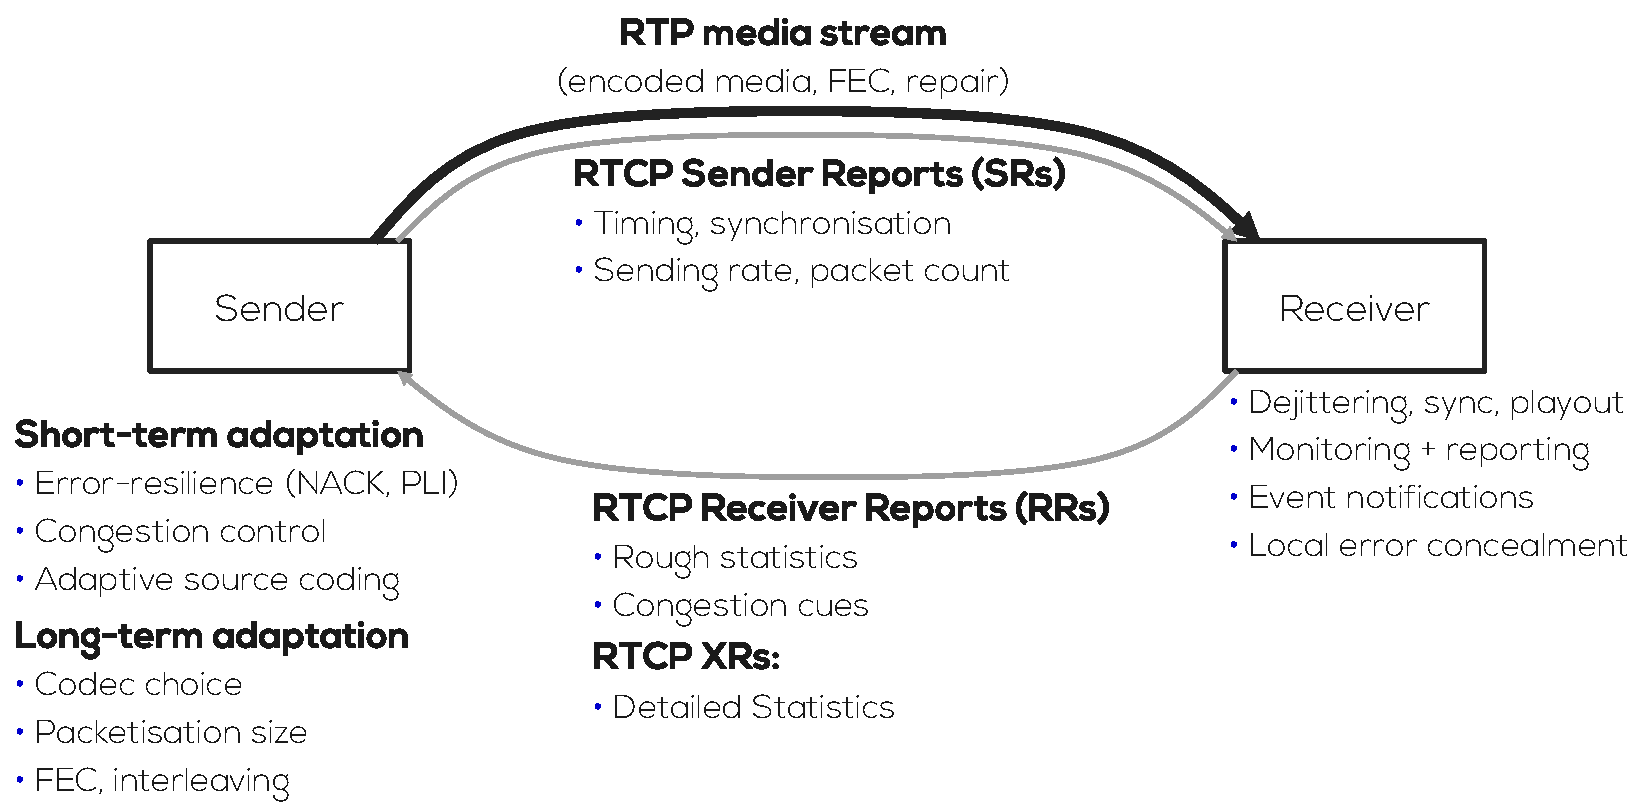
\includegraphics[width=\textwidth]{chap3-fig-rtp-rtcp}
}
\caption{RTP and RTCP for adaptive real-time applications.{\scriptsize Source:
J\"org Ott, ``Networked Multimedia Protocols and Systems''}.}
\label{fig:3:rtp:model}
\end{figure}

Figure~\ref{fig:3:rtp.hdr} describes the RTP packet header format. The
\textit{synchronization source} (SSRC) assists in determining the source
endpoint, typically useful when an endpoint sends multiple media streams that
need to be synchronized (e.g., audio and video lip-sync). The \textit{RTP
timestamp} assists in playing out the received packets at the appropriate
instance of time and recomposing the media frame from RTP packets. The
\textit{RTP sequence number} assists in identifying the lost packets and 
re-ordering packets in the case of out-of-order packet arrival. Lastly, RTP uses
the \textit{`payload type'} (PT) to describe the encoding of the media data it is
carrying. Consequently, each codec needs to specify its corresponding payload
format.

% \begin{figure}[!h]
% \centerline{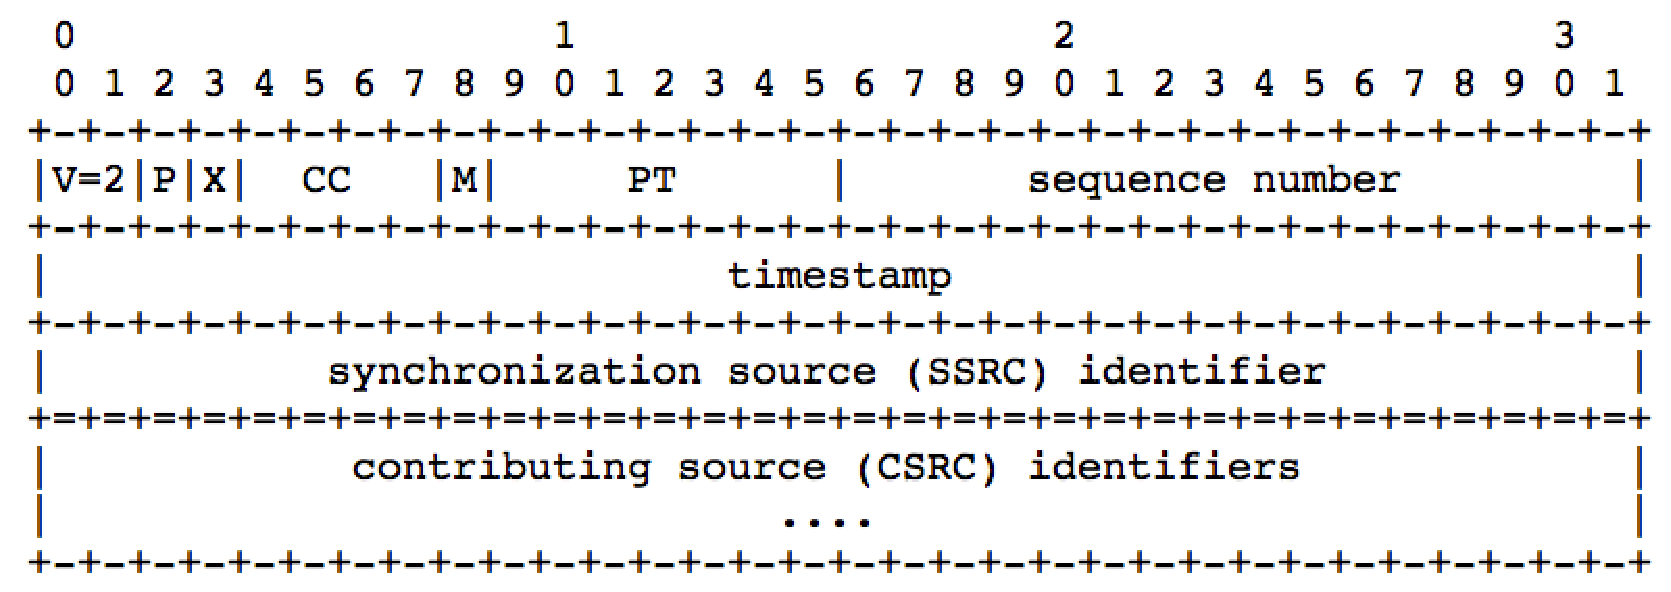
\includegraphics[width=\textwidth]{chap3_fig_hdr_rtp}}
% \caption{shows the RTP packet format that encapsulates the media data.}
% \label{fig:3:rtp.hdr}
% \end{figure}

\begin{figure}[!h]
\begin{spacing}{0.5}
\centering
{\small
\begin{verbatim}
    0                   1                   2                   3
    0 1 2 3 4 5 6 7 8 9 0 1 2 3 4 5 6 7 8 9 0 1 2 3 4 5 6 7 8 9 0 1
   +-+-+-+-+-+-+-+-+-+-+-+-+-+-+-+-+-+-+-+-+-+-+-+-+-+-+-+-+-+-+-+-+
   |V=2|P|X|  CC   |M|     PT      |       sequence number         |
   +-+-+-+-+-+-+-+-+-+-+-+-+-+-+-+-+-+-+-+-+-+-+-+-+-+-+-+-+-+-+-+-+
   |                           timestamp                           |
   +-+-+-+-+-+-+-+-+-+-+-+-+-+-+-+-+-+-+-+-+-+-+-+-+-+-+-+-+-+-+-+-+
   |           synchronization source (SSRC) identifier            |
   +=+=+=+=+=+=+=+=+=+=+=+=+=+=+=+=+=+=+=+=+=+=+=+=+=+=+=+=+=+=+=+=+
   |            contributing source (CSRC) identifiers             |
   |                             ....                              |
   +-+-+-+-+-+-+-+-+-+-+-+-+-+-+-+-+-+-+-+-+-+-+-+-+-+-+-+-+-+-+-+-+
\end{verbatim}
}
\end{spacing}
\caption{The RTP packet format that encapsulates the media data.}
\label{fig:3:rtp.hdr}
\end{figure}


\begin{figure}[!h]
\begin{spacing}{0.5}
{\footnotesize
\begin{verbatim}
          0                   1                   2                   3
          0 1 2 3 4 5 6 7 8 9 0 1 2 3 4 5 6 7 8 9 0 1 2 3 4 5 6 7 8 9 0 1
         +-+-+-+-+-+-+-+-+-+-+-+-+-+-+-+-+-+-+-+-+-+-+-+-+-+-+-+-+-+-+-+-+
  header |V=2|P|    RC   |   PT=SR=200   |             length            |
         +-+-+-+-+-+-+-+-+-+-+-+-+-+-+-+-+-+-+-+-+-+-+-+-+-+-+-+-+-+-+-+-+
         |                         SSRC of sender                        |
         +=+=+=+=+=+=+=+=+=+=+=+=+=+=+=+=+=+=+=+=+=+=+=+=+=+=+=+=+=+=+=+=+
  sender |              NTP timestamp, most significant word             |
  info   +-+-+-+-+-+-+-+-+-+-+-+-+-+-+-+-+-+-+-+-+-+-+-+-+-+-+-+-+-+-+-+-+
         |             NTP timestamp, least significant word             |
         +-+-+-+-+-+-+-+-+-+-+-+-+-+-+-+-+-+-+-+-+-+-+-+-+-+-+-+-+-+-+-+-+
         |                         RTP timestamp                         |
         +-+-+-+-+-+-+-+-+-+-+-+-+-+-+-+-+-+-+-+-+-+-+-+-+-+-+-+-+-+-+-+-+
         |                     sender's packet count                     |
         +-+-+-+-+-+-+-+-+-+-+-+-+-+-+-+-+-+-+-+-+-+-+-+-+-+-+-+-+-+-+-+-+
         |                      sender's octet count                     |
         +=+=+=+=+=+=+=+=+=+=+=+=+=+=+=+=+=+=+=+=+=+=+=+=+=+=+=+=+=+=+=+=+
  report |                 SSRC_1 (SSRC of first source)                 |
  block  +-+-+-+-+-+-+-+-+-+-+-+-+-+-+-+-+-+-+-+-+-+-+-+-+-+-+-+-+-+-+-+-+
    1    | fraction lost |       cumulative number of packets lost       |
         +-+-+-+-+-+-+-+-+-+-+-+-+-+-+-+-+-+-+-+-+-+-+-+-+-+-+-+-+-+-+-+-+
         |           extended highest sequence number received           |
         +-+-+-+-+-+-+-+-+-+-+-+-+-+-+-+-+-+-+-+-+-+-+-+-+-+-+-+-+-+-+-+-+
         |                      interarrival jitter                      |
         +-+-+-+-+-+-+-+-+-+-+-+-+-+-+-+-+-+-+-+-+-+-+-+-+-+-+-+-+-+-+-+-+
         |                         last SR (LSR)                         |
         +-+-+-+-+-+-+-+-+-+-+-+-+-+-+-+-+-+-+-+-+-+-+-+-+-+-+-+-+-+-+-+-+
         |                   delay since last SR (DLSR)                  |
         +=+=+=+=+=+=+=+=+=+=+=+=+=+=+=+=+=+=+=+=+=+=+=+=+=+=+=+=+=+=+=+=+
  report |                 SSRC_2 (SSRC of second source)                |
  block  +-+-+-+-+-+-+-+-+-+-+-+-+-+-+-+-+-+-+-+-+-+-+-+-+-+-+-+-+-+-+-+-+
    2    :                               ...                             :
         +=+=+=+=+=+=+=+=+=+=+=+=+=+=+=+=+=+=+=+=+=+=+=+=+=+=+=+=+=+=+=+=+
         |                  profile-specific extensions                  |
         +-+-+-+-+-+-+-+-+-+-+-+-+-+-+-+-+-+-+-+-+-+-+-+-+-+-+-+-+-+-+-+-+
\end{verbatim}
}
\end{spacing}
\caption{The RTCP packet format for carrying the Sender Report (SR) and
the Receiver Report (RR). The SR carries transport statistics and enables 
stream synchronization, while the RR carries the receiver transport 
characteristics.}
\label{fig:3:rtcp.hdr}
\end{figure}

% \begin{figure}[!h]
% \centering{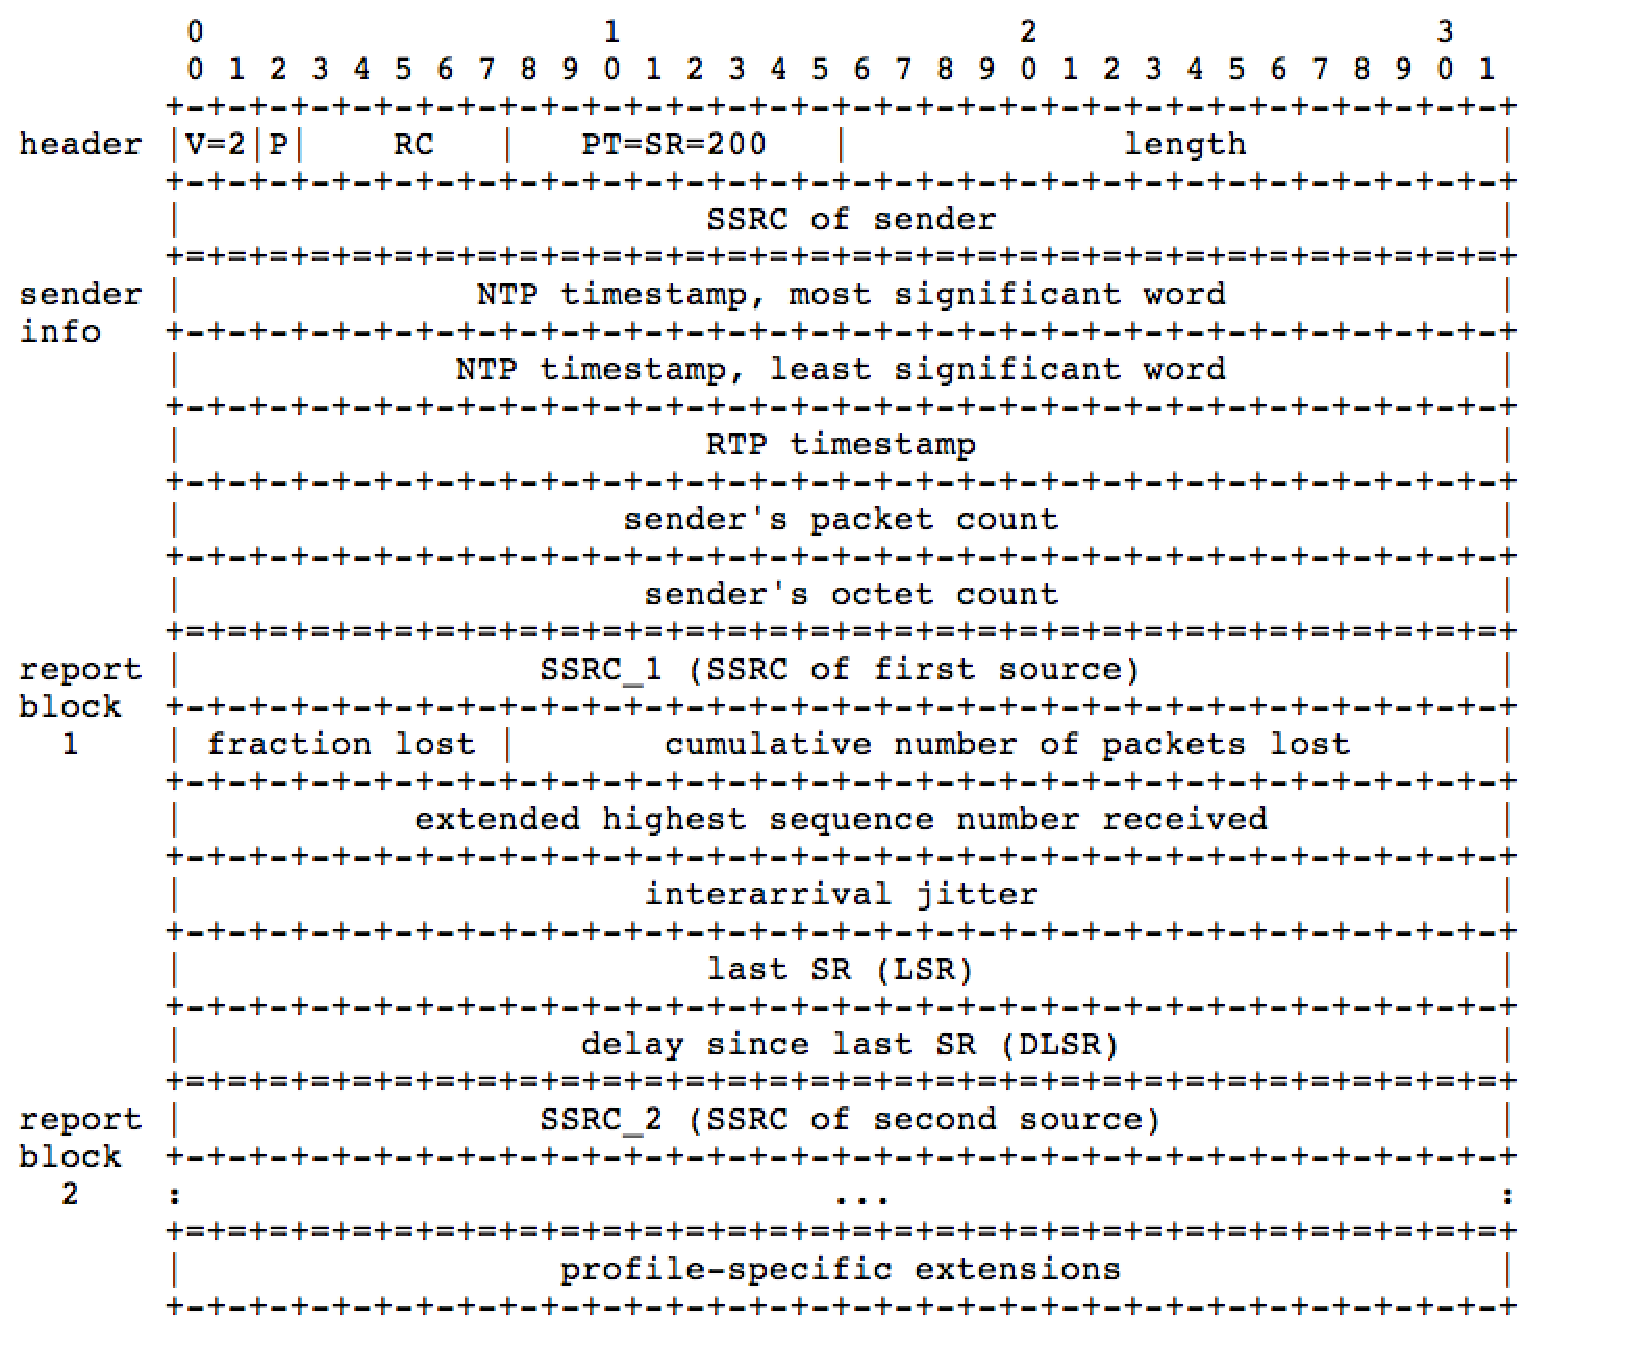
\includegraphics[width=\textwidth]{chap3_fig_hdr_rtcp}}
% \caption{shows the RTCP packet format for carrying the Sender Report (SR) and
% the Receiver Report (RR). The SR carries transport statistics and enables 
% stream synchronization, while the RR carries the receiver transport 
% characteristics.}
% \label{fig:3:rtcp.hdr}
% \end{figure}

The receiver measures the incoming streams and reports the coarse-grained
transport statistics in an RTCP Receiver Report (RR). The RTCP RR contains the
current loss fraction, jitter, and the highest sequence number received, and it
facilitates in calculating the round-trip time (RTT). The sender uses RTCP Sender Reports (SRs)
to assist in synchronizing the media streams (audio and video) by relating the
RTP timestamps of the individual media streams to the wall clock time (NTP)
and notifying the receiver about the current packet rate and bit rate.
Figure~\ref{fig:3:rtcp.hdr} shows the RTCP packet header format for a
interactive unicast media stream (i.e., both sending and receiving media).

\section{RTP Payload Formats}

The general principle for defining payload formats/types is to 
identify the encoding of the media packets. These encodings are either  
codec-specific (e.g., H.264, H.263, H.261, MPEG-2, JPEG, G.711, G.722, AMR, etc.),
or generic (e.g., Forward Error Correction (FEC), NACK, multiplexed streams).
Typically, a payload document specifies a well-defined packet format for media
codecs; it also defines \emph{aggregation rules} for codecs that produce
several small frames (e.g., audio) compared to the IP Maximum Transmission
Unit (MTU), and \emph{fragmentation rules} for codecs that produce large frames
(e.g., I-frames by video codecs). The main reason for fragmenting large
frames into smaller packets and not rely on IP fragmentation is that IP
fragmented packets are commonly discarded in the network, especially by NATs
or firewalls.

% Usually the RTP header is immediately followed by
% payload-specific header (payload format) and then by the media data. This
% allows the sending endpoint to semantically fragment large packets, which
% simplifies processing and decoding at the receiver (i.e., be able to decode
% individual packets without relying on receiving other packets).

\begin{figure}[!h]
\begin{spacing}{0.5}
{\footnotesize
\begin{verbatim}
    0                   1                   2                   3
    0 1 2 3 4 5 6 7 8 9 0 1 2 3 4 5 6 7 8 9 0 1 2 3 4 5 6 7 8 9 0 1
   +-+-+-+-+-+-+-+-+-+-+-+-+-+-+-+-+-+-+-+-+-+-+-+-+-+-+-+-+-+-+-+-+
   |V=2|P|X|  CC   |M|     PT      |       sequence number         |
   +-+-+-+-+-+-+-+-+-+-+-+-+-+-+-+-+-+-+-+-+-+-+-+-+-+-+-+-+-+-+-+-+
   |                           timestamp                           |
   +-+-+-+-+-+-+-+-+-+-+-+-+-+-+-+-+-+-+-+-+-+-+-+-+-+-+-+-+-+-+-+-+
   |           synchronization source (SSRC) identifier            |
   +=+=+=+=+=+=+=+=+=+=+=+=+=+=+=+=+=+=+=+=+=+=+=+=+=+=+=+=+=+=+=+=+
   |                 Payload Format-Specific Header                |
   +               +-+-+-+-+-+-+-+-+-+-+-+-+-+-+-+-+-+-+-+-+-+-+-+-+
   |               |                                               |
   +-+-+-+-+-+-+-+-+                                               +
   |                           Media Data                          |
   +                                                               +
   |                                                               |
   +-+-+-+-+-+-+-+-+-+-+-+-+-+-+-+-+-+-+-+-+-+-+-+-+-+-+-+-+-+-+-+-+
\end{verbatim}
}
\end{spacing}
\caption{Packet structure of an RTP packet encapsulating the
payload-specific header and the associated media data.}
\label{fig:3:pt.fmt}
\end{figure}

% \begin{figure}[!t]
% \centerline{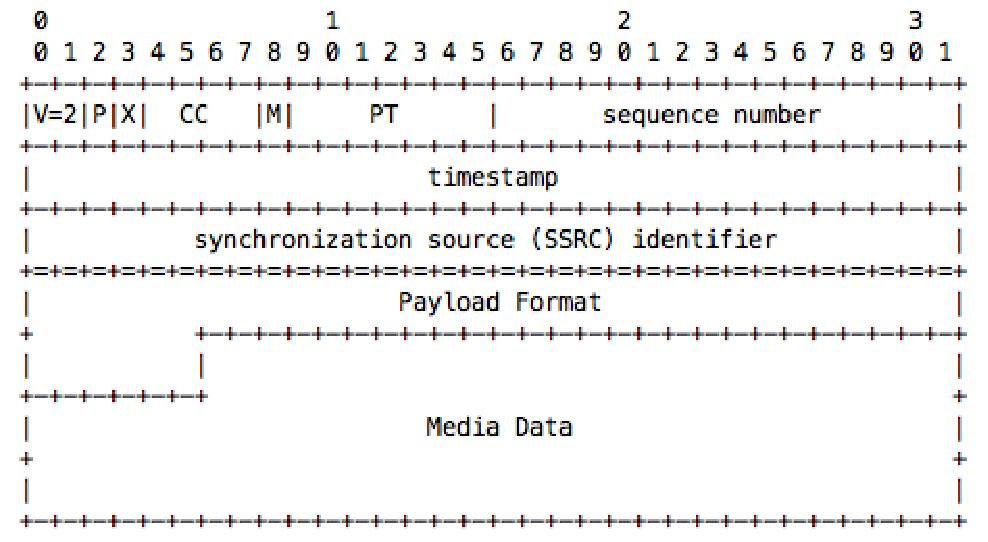
\includegraphics[width=\textwidth]{chap3_fig_hdr_pt_fmt}}
% \caption{shows the packet structure of an RTP packet encapsulating the
% payload-specific header and the associated media data.}
% \label{fig:3:pt.fmt}
% \end{figure}

\section{RTP Header Extensions}

RTP header extensions carry media-independent information, i.e., data that may
be generically applicable to multiple payload formats (e.g., timing
information), and needs to be reported more frequently than RTCP reports are
emitted. A commonly-cited example is the sending of NACK packets for interactive video,
where media flows in both directions and RTP packets are generated every tens
of milliseconds. In this case, the RTP header extension can indicate which sequence numbers
were correctly received or lost, thereby not completely relying on the RTCP
receiver reports to send NACKs or ACKs.

The advantage of using header extensions is that they are backwards
compatible, i.e., an endpoint that does not understand them is able ignore
them. Some current use-cases for RTP header extensions include reporting the
network send timestamp: instead of bursting packets from a large frame on to
the network, the sender paces these packets.  Another example is equalizing a
client's audio levels across multiple streams in a video conference. Lastly,
RTP header extensions are generic, there is no need to redefine the same extension
for each media codec.

\section{RTCP Reporting Interval}
% timing

A closed control loop is formed by sending RTP media packets and receiving
RTCP feedback packets. The RTCP feedback interval is typically limited to a
small fraction of the session bandwidth (\emph{session\_bw}) as not to affect the media traffic.
The RTCP reporting interval is determined by the number of SSRCs in the
session (denoting the session size), and the chosen session bandwidth. The
session bandwidth (\emph{session\_bw}) is expected to be divided amongst the participants, but
oftentimes it is calculated as the sum of the average throughput of the
senders expected to be concurrently active. In the case of an audio conference,
the session bandwidth would be one sender's bandwidth, but for a video
conference, the session bandwidth would vary depending on the number of participants displayed on
the user interface. Consequently, the session bandwidth is supplied by the
session management layer so that the same value for the RTCP interval is calculated for each participant.


The recommended fraction of the session bandwidth allocated for control
traffic is 5\,\%. For many scenarios, including large conferences, where there
are a large number of receivers but a small number of senders, it is
recommended that a quarter of the reporting bandwidth (\emph{rtcp\_bw}) be
shared equally by the senders and the remaining three-quarters by the receivers. The
main reason for this allocation ratio is to allow newly-joining participants to quickly receive the
CNAME and synchronization timestamps from the Sender Reports (SRs). 
For new participants (even if they are just receivers), the RTCP
interval is halved to quickly declare their presence.  Lastly, the recommended
value for a fixed minimum RTCP interval is 5 seconds, while the value for a
reduced minimum is $\frac{360}{session\_bw}s$.  The fixed minimum RTCP
interval of \emph{5\,s} is suitable for unidirectional links or for sessions
that do not require monitoring of the reception quality statistics (e.g., IPTV),
while the reduced minimum RTCP interval is also suitable for participants in a
unicast bidirectional multimedia session. The reduced minimum RTCP interval
is suitable for sending timely feedback messages to either perform congestion
control or error repair; the interval is shorter than \emph{5\,s} for session
bandwidths greater than \emph{72\,kbps}.

% avpf

If an endpoint detects packet loss or the onset of congestion midway through a
reporting interval, the base RTP specification~\cite{rfc3550} (AVP profile)
does not allow the RTCP reports to be sent early and the endpoint has to wait for
the next scheduled RTCP report. In this case, the slow control loop causes
instability and oscillation in the media bit rate. To overcome this
shortcoming, endpoints implement the Extended RTP Profile for RTCP-Based
Feedback (AVPF profile)~\cite{rfc4585}, an extension to RTP's default timing
rules, to enable rapid feedback. This profile allows the endpoint to adjust the
RTCP reporting interval to send the RTCP feedback reports earlier than the
next scheduled RTCP report, sometimes even immediately, as long as the reporting
interval on average remains the same. Figure~\ref{fig:3:avpf.interval} shows
that with AVP profile, the endpoint reports at regular intervals, whereas with AVPF
the endpoint it gets the opportunity to send feedback early in every other reporting
interval. Along with the possibility of providing timely feedback, the AVPF
profile also defines a suite of error-resilience feedback messages, namely,
Negative Acknowledgments (NACK), Picture Loss Indication (PLI), Slice Loss
Indication (SLI), and the Reference Picture Selection Indication (RPSI).

\begin{figure}[!t]
\centering{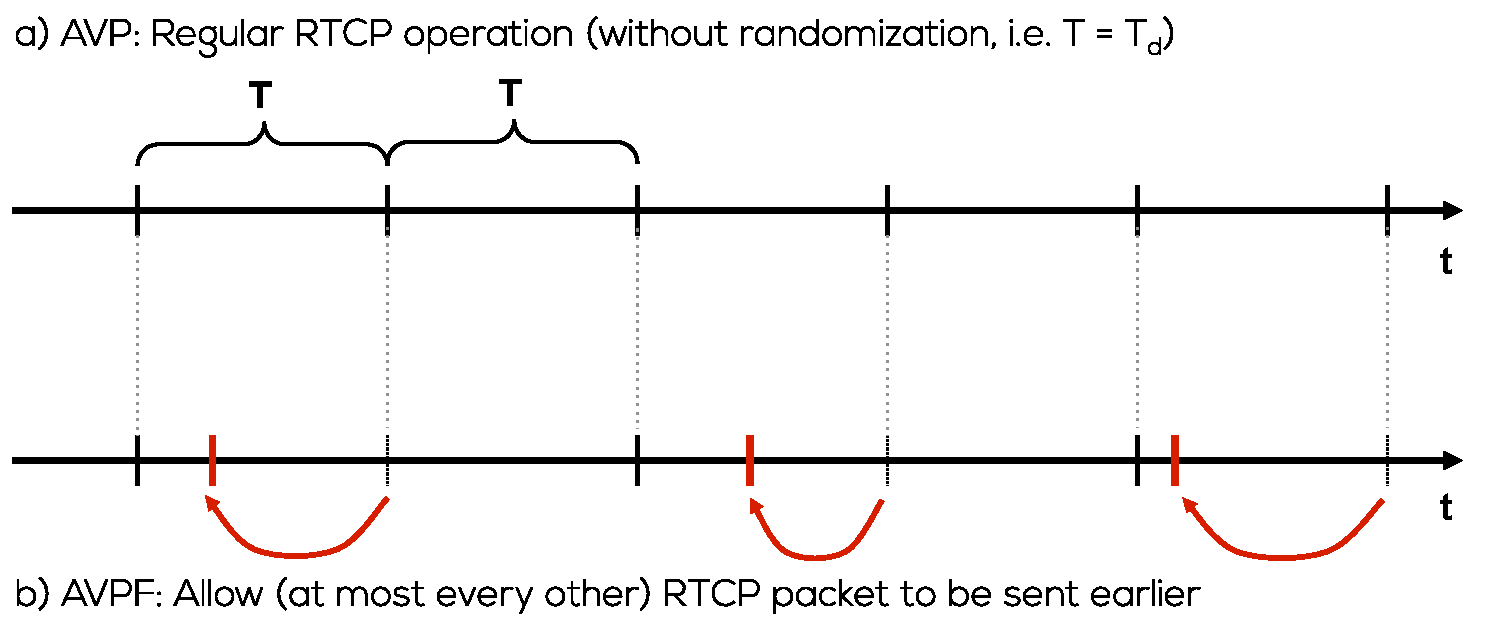
\includegraphics[width=\textwidth]{chap3-fig-avpf-rtcp}}
\caption{The RTCP reporting interval as defined in a) AVP, b) AVPF.}
\label{fig:3:avpf.interval}
\end{figure}




\section{RTCP Extended Reports (XRs) for Performance Monitoring}

Endpoints use RTCP Extended Reports (XRs)~\cite{rfc3611} to describe complex
metrics that are not exposed by the RTCP Receiver Report (RR). Some examples of
XRs relevant to performance monitoring and congestion control are: de-jitter
buffer metrics~\cite{rfc7005}, Packet Delay Variation (PDV)~\cite{rfc6798},
delay metrics~\cite{rfc6843}, burst-gap discard~\cite{rfc7003}, burst-gap
loss~\cite{rfc6958}, Run-Length Encoded (RLE) loss~\cite{rfc3611}, discard
RLE~\cite{rfc7097}, the number of discarded packets~\cite{rfc7002} and
bytes~\cite{rfc7243}, summary statistics~\cite{rfc7004},
Quality of Experience (QoE)~\cite{draft.xr.qoe}, and loss
concealment~\cite{draft.xr.conceal}, etc. RTP allows for new metrics to be
defined; the main requirement is to document what is measured, how it is
measured and how it is reported to the other endpoints.


% The RTCP Extended Reports (XR) [RFC3611] allow reporting of more
% complex and sophisticated reception quality metrics, but do not
% change the RTCP timing rules.  RTCP extended reports of potential
% interest for congestion control purposes are the extended packet
% loss, discard, and burst metrics [RFC3611],
% [I-D.ietf-xrblock-rtcp-xr-discard],
% [I-D.ietf-xrblock-rtcp-xr-discard-rle-metrics],
% [I-D.ietf-xrblock-rtcp-xr-burst-gap-discard],
% [I-D.ietf-xrblock-rtcp-xr-burst-gap-loss]; and the extended delay
% metrics [RFC6843], [RFC6798].


\section{Codec Control Messages}
% codec control

Sometimes an endpoint needs to configure or notify the other endpoint's codec.
These messages are broadly classified as \emph{Transport Layer} and \emph
{Payload-specific} feedback messages~\cite{rfc4585, rfc5104}. The transport
layer messages are: Temporary Maximum Media Stream Bit Rate Request (TMMBR)
and Temporary Maximum Media Stream Bit Rate Notification (TMMBN). The
receiving endpoint uses the TMMBR message to configure the maximum encoding
bit rate of the media stream, while the sending endpoint uses the TMMBN to
inform the receiver of the updated bit rate. Therefore, transport layer
feedback messages are intended to transmit general purpose feedback messages,
independent of any particular codec or application.

On the other hand, the payload-specific feedback messages carry information
specific to a certain payload type and are acted upon by the codec layer. Some
examples of these type of messages are: Full Intra Request (FIR), 
temporal-spatial tradeoff, frame rate, frame size, maximum packet size or packet rate,
etc.~\cite{draft.avt.cop}.

\section{Reduced-Size RTCP Reports}
% non-compound feedback

An endpoint sends RTCP feedback as a \emph{compound}, or \emph{minimal}, RTCP
packet. A \emph{compound RTCP packet} as defined in~\cite{rfc3585} contains
at least a sender report (SR) or a receiver report (RR) or both, followed by
a Source Description (SDES) and any additional XR blocks. A \emph{minimal RTCP
packet} is one that contains an SR and/or RR, and is followed by an SDES
containing just the canonical name (CNAME)\footnote{The real name
(identifier) used to describe the source; it can be in any form desired by the
user. Of the SDES items (username, email, phone, geolocation, etc.), it is 
compulsory to include CNAME in every RTCP packet.}. Hence, every compound RTCP
packet is a minimal RTCP packet with additional report blocks. A typical RTCP
packet size for conversational multimedia streams is 80 bytes (RTCP=8, SR=20,
RR=24, SDES/CNAME =28).

Including any of the additional SDES items or adding XR blocks makes the
compound RTCP packet very large. On low bit rate links, these large compound
RTCP packets may introduce more delay. Therefore, it may be desirable to
logically fragment the report blocks in a compound RTCP packet and send them
independently. These fragmented report blocks are called \emph {reduced-size
RTCP packets}~\cite{rfc5506}. Unlike compound RTCP packets, to transmit a
reduced-size RTCP packet an endpoint does not need to include the minimal RTCP
report. However, when using reduced-size RTCP packets, minimal packets need to
be sent once in a while to keep the CNAME-SSRC binding alive.

Reduced-size RTCP reports are beneficial in wireless networks where the packet
loss rate increases with the packet size, i.e., larger-sized packets are more
susceptible to being dropped compared with smaller-sized packets. Additionally, smaller
packets have shorter serialization time, i.e., the amount of time it takes for
the endpoint to put the data packet onto the link is short.

The main reasons for the application to use reduced-size RTCP reports are:
1) to notify the other endpoint of events. Using the signaling channel would
incur at least one RTT while implementing it as an RTCP extension would merely
incur a one-way delay. 2) to send codec control (e.g., TMMBR) or feedback (e.g.,
NACK, RPSI) messages. These reduced-size messages are more likely to be
transmitted more often and with as little delay as possible, especially since
these types of messages are more likely to be sent when link conditions are
poor.


% relationship with SDP
\section{Session Setup}

% SDP O/A, declarative SDP, RTCP notify

There are several ways to set up an interactive or conversational multimedia
session, for example by implementing one of the following: H.323~\cite{H.323},
Session Initiation Protocol (SIP)~\cite{rfc3261}, or Jingle~\cite{XEP-0166}, an
extension to the Extensible Messaging and Presence Protocol
(XMPP)~\cite{rfc6120}.

SIP uses the Session Description Protocol (SDP)~\cite{rfc4566} to describe the
endpoint's transport and media capabilities. An SDP description defines a
single multimedia session, i.e., an association between a set of participants.
It may, however, carry multiple media streams in the session.

\begin{figure}[!h]
\centerline{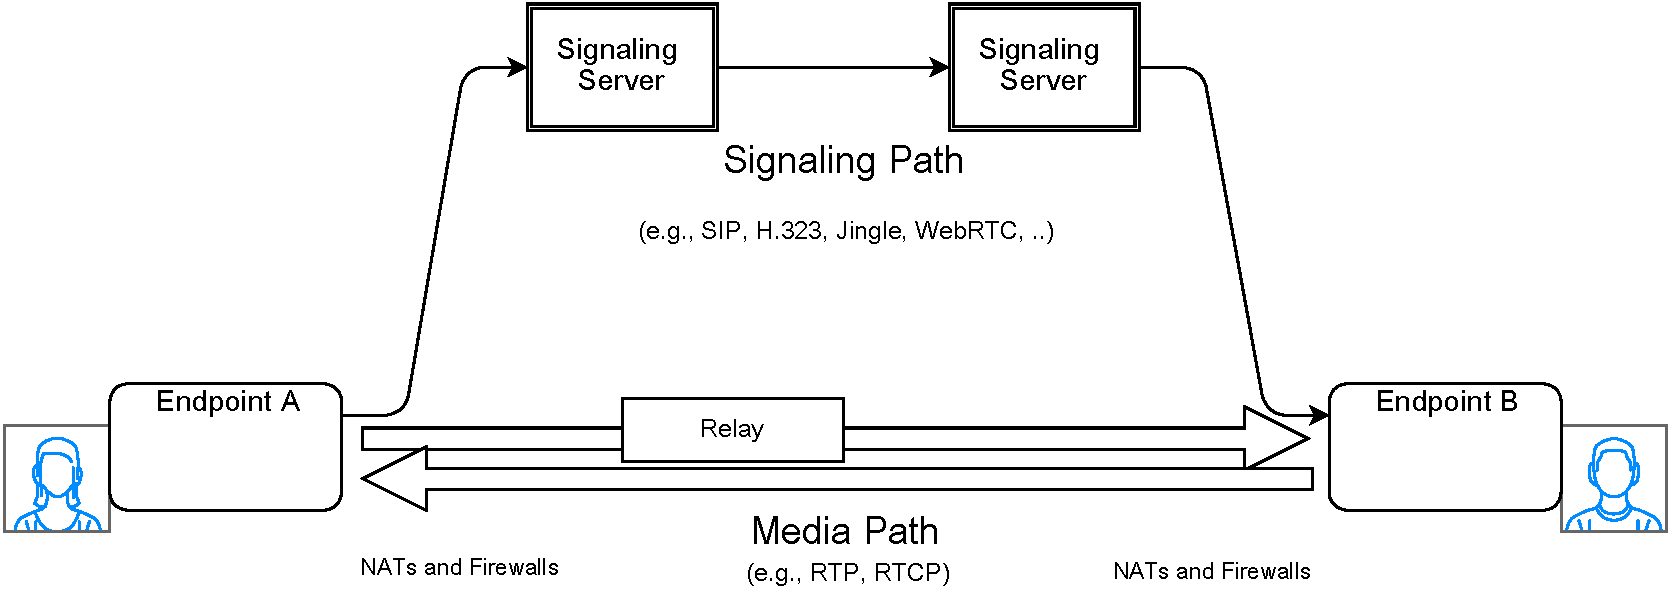
\includegraphics[width=\textwidth]{chap3-fig-sig-med}}
\caption{The signaling and media paths between two endpoints engaging in
a video call.}
\label{fig:3:sig.media}
\end{figure}


The transport details in the SDP are mainly split into two parts: the protocol
for delivering media packets (currently, TCP, UDP, or SCTP), and the 
IP address of the endpoint. The protocol to deliver the media packets is
chosen by the application, but identifying the IP address and port of an
endpoint is a bit complex. It first requires gathering the endpoint's multiple
IP addresses and later exchanging them with the other endpoints to establish
connectivity.

Multiple IP addresses arise not only from multiple interfaces but also from
the presence of NAT devices in the network, which may change the IP address of
the outgoing packets. Since interactive media calls are between endpoints and
media streams may eventually traverse a NAT at both ends, in some cases, the
only way to deliver media packets between two endpoints would is by using
a relay\footnote{Traversal Using Relays around NAT (TURN)} on the public
Internet. Hence, the endpoint needs to discover its 2-tuple \texttt{[IP
address:port]} on the host, which is relatively easy followed by the public 
address, if behind a NAT~\cite{rfc5389}. Discovering an endpoint's public address
requires contacting a publicly-hosted STUN\footnote{Session Traversal
Utilities for NAT (STUN).} server and comparing the endpoint's
host addresses with the one observed by the STUN server. Lastly, the endpoint
discovers the address allocated by the TURN relay~\cite{rfc5766} and notifies
the other endpoints about its transport details. This collection of 2-tuples
is known as \emph{candidates}. First, each endpoint sorts its candidates
in decreasing order of priority and exchanges these candidate addresses in the
SDP with the other endpoint. On receiving the list of candidates, the endpoints
probes between each combination of addresses in the two candidate
lists; a pair of addresses is called a \emph{candidate pair}. The endpoint
chooses the first candidate pair that successfully establishes connectivity
(\emph{aggressive nomination}). This process of performing pair-wise
\emph{connectivity checks} is called Interactive Connectivity Establishment
(ICE)~\cite{rfc5245, rfc6544} and it relies on the STUN protocol~\cite{rfc5389} to establish connectivity
across a NAT. In case direct connectivity between the two endpoints fails 
to be established, the individual endpoints use the \emph{Traversal Using Relays
around NAT} (TURN) server and the associated protocol~\cite{rfc5766} to relay
media packets between them. Similar to the STUN server, the TURN
server is hosted on the public Internet.

% Depending on the type of NAT device (full-cone, address- or port-restricted
% cone, symmetric).

\begin{figure}[!h]
{\small
\begin{verbatim}
        v=0
        o=jdoe 2890844526 2890842807 IN IP4 10.0.1.1
        s=
        c=IN IP4 192.0.2.3
        t=0 0
        a=ice-pwd:asd88fgpdd777uzjYhagZg
        a=ice-ufrag:8hhY
        m=audio 45664 RTP/AVP 0
        a=rtpmap:0 PCMU/8000
        a=candidate:1 1 UDP 2130706431 10.0.1.1 8998 typ host
        a=candidate:2 1 UDP 1694498815 195.148.127.98 45664 typ srflx 
            raddr 10.0.1.1 rport 8998
\end{verbatim}
}
\caption{Sample SDP containing the sender's transport and media capabilities.}
\label{fig:3:sdp}
\end{figure}

The second part of SDP carries the media capabilities, together with the 
transport parameters, that bind the SDP to the Offer/Answer model. In the O/A
model, the sending endpoint \emph{offers} to the receiver a set of media
capabilities in decreasing order of preference, typically, multiple options of
audio/video codecs and ICE candidates. On receiving the sender's capabilities,
the receiver compares its media capabilities with the sender's and responds
with the one that best fits the receiver's requirements (\emph{answer}). The
\emph{offer is rejected} if the receiver is unable to pick any
of the options provided by the sender, or if the ICE connectivity checks fail.
Hence, the application at the sender needs to pick a minimum number of widely-available 
audio and video codecs to avoid negotiation failure. If the
\emph{offer is accepted}, both endpoints then know the following: 1) which
audio and/or video codecs to use, 2) the payload types of the encoded media
streams (possibly even their respective SSRCs), 3) to which IP address and
port number to send the media stream, 4) the media session bandwidth, if
indicated, and 5) the encryption keys, if encrypting traffic.

\begin{figure}
\centering{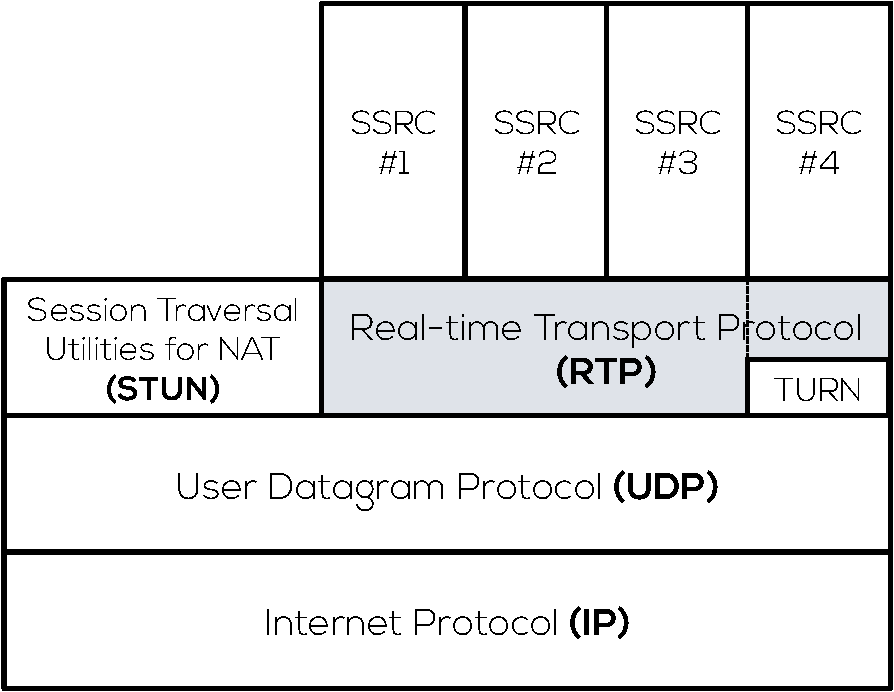
\includegraphics[width=0.9\textwidth]{chap3-fig-rtp-stack}}
\caption{Relationship of RTP with STUN, TURN, DTLS and the signaling protocol.}
\label{fig:3:rtp-stack}
\end{figure}

Figure~\ref{fig:3:rtp-stack} shows the relationship of the RTP stack with the
rest of the IP stack. RTP is usually transmitted over UDP, but under some
constrained situations (e.g., restrictive firewalls or NATs), RTP may be
encapsulated in TCP~\cite{rfc3550}. STUN~\cite{rfc5389} is used by ICE to
discover the presence of a NAT device and obtain the mapped (public) IP
address. When using a TURN relay server (in the presence of symmetric NATs or
when concealing the host address of the caller for privacy reasons), the RTP
packets are encapsulated inside the TURN's \emph{ChannelData}
message~\cite{rfc5766}. In Figure~\ref{fig:3:rtp-stack}, four media streams
(SSRC \#1-4) are transmitted by RTP over UDP, but two streams (SSRC \#1-2) are
relayed through a TURN server. Secure RTP (SRTP)~\cite{rfc3611} is a security
framework that provides confidentiality by encrypting RTP payload (not the RTP
headers) and supports source origin authentication. While SRTP is not the only
security mechanism for RTP~\cite{draft.srtp-not-must}, it is widely
applicable, especially to voice telephony and group communication. However,
the main challenge for SRTP is key management~\cite{draft.sec-opts}, since
many options exist (e.g., SRTP over DTLS in WebRTC~\cite{rfc5763}, MIKEY in
SIP~\cite{rfc3830}, Security Description in SDP~\cite{rfc4566},
ZRTP~\cite{RFC6189}, etc.).

\section{Summary}

In this chapter we introduced the basic features of RTP and RTCP; we discussed
the limits on reporting interval and the numerous RTP and RTCP extensions.
The introduction to RTP and RTCP largely provides context and helps understand
the design constraints  for multimedia congestion control which are discussed 
in more detail in the forthcoming chapters.


\chapter{Congestion Control Framework for Real-time Communication}
\label{chap:cc.fw}
In the forthcoming deployment of WebRTC systems, we speculate that high
quality\footnote{normally, high quality corresponds to an increase in required
bandwidth.} video conferencing will see wide-scale adoption. To assure
stability of the network (and avoid congestion collapse), these real-time
communication systems are required to implement some kind of congestion
control for their RTP-based media traffic.

RTP transmits the media data over IP using a variety of transport layer
protocols such as UDP, TCP, and Datagram Congestion Control Protocol (DCCP).
Consequently, congestion control for RTP-based media flows is implemented
either in the application or the media flows are transmitted over
congestion-controlled transport (TCP or DCCP). While using a congestion-controlled 
transport may be safe for the network, it is sub-optimal for the
media quality unless the congestion-controlled transport is designed to carry
media flows. Unfortunately, TCP is only suitable for interactive multimedia
for paths with very low RTT (<100\,\emph{ms} )~\cite{Brosh:tcp-real-time}, and
DCCP packets have problems with NAT traversal~\cite{schier:DCCP} unless DCCP is
encapsulated in UDP~\cite{RFC6773}.

This motivates the need for a UDP congestion control algorithm, where the
congestion control is implemented between the application and the
underlying transport, thereby taking into
account both the application's and the transport's requirements or constraints
and with appropriate trade-off. In this thesis, we consider congestion
control for unicast RTP traffic running over the best-effort IP network.

% CC should not cause queuing delay. Or define low-latency operation of
% multimedia cc.

Endpoints rely on RTCP feedback from the receiver to implement congestion
control. Hence, the congestion control should consider the following three aspects
in its design: congestion cues to report, block size of each report or the
overhead incurred by reporting a cue, and the frequency of these feedback
reports. In the following subsections, we describe the interaction between the
application and the congestion control, list common congestion cues, discuss
the feedback reporting frequency, the classification of cues, the metrics and
criteria to evaluate congestion control proposals, and lastly, we discuss the
RTP circuit breaker which stops transmission permanently after observing
prolonged congestion.

\section{Adaptive Multimedia Systems}
\label{fw.amusys}

Any real-time communication endpoint is made up of three basic components:
codec (encoder and decoder), transport (RTP and UDP) and the application
preferences (user and application settings, system policies, capturing and
rendering constraints, etc.). The codec encodes and decodes a media stream. A
typical application comes with at least one codec each for audio and video. 
The application may also implement several other media codecs so that 
it is capable of inter-operating
with several different types of endpoints. The transport is mainly made up of
RTP, which packetizes and depacketizes the media and UDP to transmit the
media. The application preferences are made up of system polices (which
interface to use? which codec to prefer?), codec settings (the
preferred or the minimum video resolution, preferred frame rate, etc.). The
application preferences may also depend on the outcome of the session
establishment, in which the participating endpoints negotiate the codec and
network settings.

\begin{figure}
  \centerline{
    \subfloat[Sending Endpoint]{
      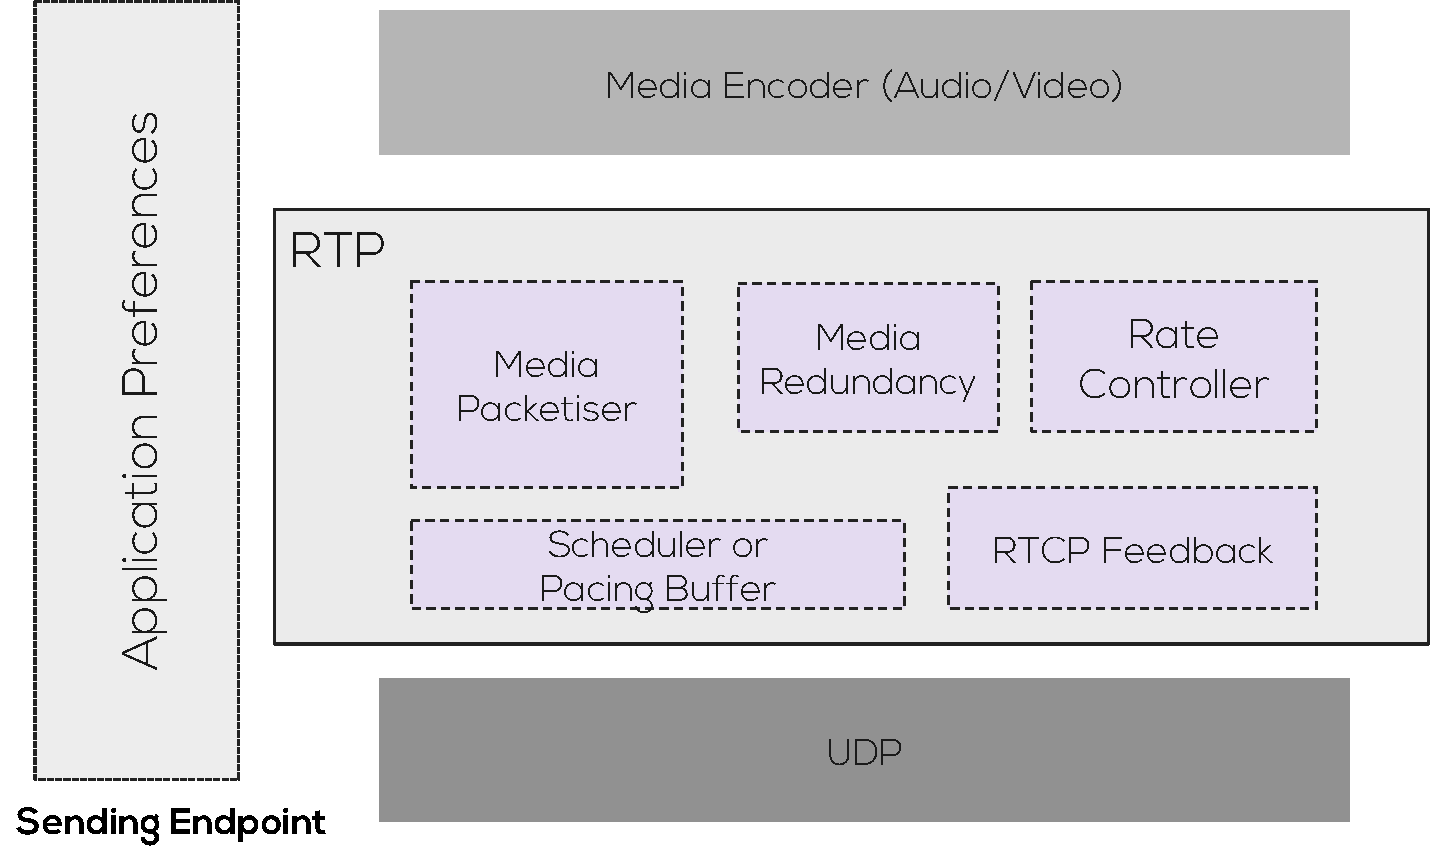
\includegraphics[width=0.66\textwidth]
      {chap4_fig_app_sender}
    }
  }
  \centerline{
    \subfloat[Receiving Endpoint]{
      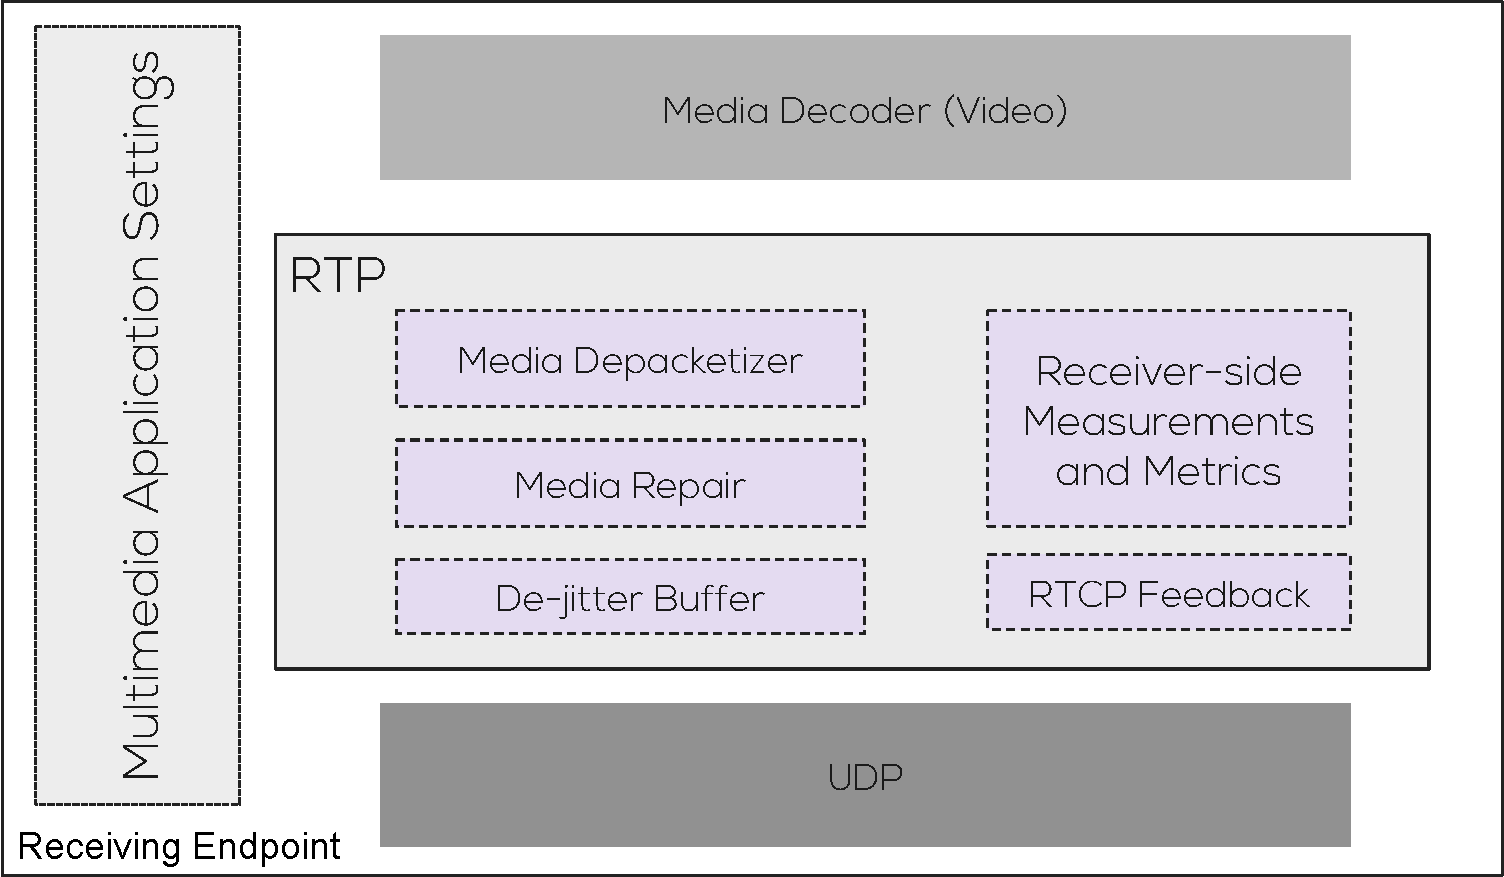
\includegraphics[width=0.66\textwidth]
      {chap4_fig_app_receiver}
    }
  }
  
  \caption{Typical architecture of a multimedia system. a) sending endpoint,
  b) receiving endpoint.}
  \label{fig:4:appint}
\end{figure}

Figure~\ref{fig:4:appint} shows a simplified architecture of a sending and
receiving endpoint; typically, a real-time multimedia application would
contain both these systems and perhaps even two of each for handling audio and
video separately. Figure~\ref{fig:4:appint} (a) depicts the features of the
sending-side RTP stack. The \emph{media packetizer} subsystem receives a video frame or a
series of audio frames from the codec, which it packetizes into RTP.  The
resulting RTP packets are then passed on to the \emph{media redundancy} subsystem to
be cached if a NACK is received or for producing FEC packets. Additionally,
the RTP packet size and count is sent to the RTCP subsystem for creating RTCP
SR packets. Simultaneously while passing the packet to the media redundancy
subsystem, the RTP packets are sent to the \emph{pacing buffer or scheduler} subsystem which
transmits the packets in a single burst or trickles them on to the network
before the next set of RTP packets are generated by the media packetizer or codec. The
sending endpoint also routinely generates and receives RTCP packets. 
The RTCP RR packets are sent to the \emph{RTCP feedback} subsystem and 
onwards to the \emph{Rate Controller} subsystem.
The rate controller monitors the congestion cues and based on the congestion control
algorithm calculates the  new target encoding rate. The codec attempts to
compress the media stream to meet the new target encoding rate in a reasonable
time frame. Figure~\ref{fig:4:appint} (b) depicts the features of the
receiving-side RTP stack. The received RTP packet is put in a \emph{dejitter buffer}
to reassemble out-of-order packets. The dejitter buffer may discard late
arriving packets and it also detects packet loss. Furthermore, the packet
sequence number, size of the packet, RTP timestamp and the reception
timestamp are passed to the \emph{RTCP feedback} subsystem, which routinely generates an
RTCP RR packet and may additionally generate requests for retransmitting
missing RTP packets. This information is also shared with \emph{receiver-side
measurements and metrics} subsystem, which may generate additional congestion
cues to be sent along with the RTCP RR as RTCP extended reports (XRs). If FEC
packets or other types of repair packets are received, they are passed on to
the \emph{media repair} subsystem which attempts to recover the missing packets in
the dejitter buffer. The dejitter buffer size is typically configured to a small value to maintain
communication interactivity, so packets are sent to the \emph{media packetizer} where
an audio or video frame is reconstructed and sent to the decoder for playback.


We identify three control loops to implement congestion
control~\cite{Singh:control.loops.api} based on the interaction between the
above components in an multimedia system~\cite{draft.rmcat.app.interaction},

\begin{enumerate}
\setlength{\itemsep}{0pt}

\item \textbf{\texttt{Codec-Sender}}: The codec adapts its encoding rate based
on the feedback from the sender. Unlike elastic traffic, the codec is unable
to produce the expected media rate immediately. Therefore, the rate-controller
needs to take into account the timeline in which the codec produces the new
rate.

\item \textbf{\texttt{Sender-Network}}: The sender packetizes media frames and
sends them over the network to the receiver. The sender may however pace the
fragmented frames on to the network instead of sending them in a single
burst. It also collects feedback messages from the receiver that may contain
congestion cues (i.e., variation in RTT, indication of lost or discarded
packets, goodput, jitter, etc.).

\item \textbf{\texttt{Receiver-Sender}}: The receiver has a playout buffer of
media data waiting to be decoded and rendered, discarding packets that arrive
late for playout, and attempting to conceal the missing packets from the
observer. The receiver also monitors the media flow for packet losses,
variation in jitter, receiver rate, goodput, etc. and reports these to the
sender to act upon.

\end{enumerate}

If an endpoint detects congestion rapidly, and the end-to-end path latency is
sufficiently low so that this information can be communicated quickly, it is
possible to change the encoding rate promptly to meet the variation in the 
end-to-end path capacity. However, in practice, this is not always possible because
\textbf{a)} it may take multiple reports or data packets to detect congestion, and
\textbf{b)} after detecting congestion, it takes at least a one-way delay (OWD)
amount of time for the receiver to report it.


\section{Congestion Cues}
\label{fw.cues}

Congestion control algorithms rely on cues to detect congestion. These cues
are detected either by the sender, receiver, or by an intermediary router. The
endpoint observes the congestion along the path and accordingly adapts the
sending rate upon receiving the congestion cues. 
Some common congestion cues are listed below:

\begin{itemize}
\setlength{\itemsep}{0pt}

\item \textbf{\texttt{Losses}}: occur when intermediate routers drop packets
from their queues (\emph{congestion loss}), or due to contention, interference
or fading on wireless link (\emph {bit-error loss}). Losses are inferred at
the receiving endpoint by gaps in RTP sequence numbers. Typically, a dejitter
buffer is used to reorder out of order packets and the fraction packet loss is
calculated at the end of each reporting interval.

\item \textbf{\texttt{Discards}}: packets that arrive too late at the receiver
to be decoded or played back may be discarded by the receiving endpoint. These
late-arriving packets are discarded by the receiver even though they are
received because packets with higher \textit{timestamps} have already been
passed to the decoder for playback. The fractional loss in the standard RTCP
RR does not identify these discarded packets as lost, hence they need to be
reported in an RTCP XRs.

\item \textbf{\texttt{Sending rate, receiver rate and goodput}}: are measured
at the sender, the receiver and at the decoder, respectively. Typically, the
sending rate is the rate at which the media bit stream is generated by the
encoder. If packets are lost in the network, the receiver rate is lower than
the sending rate. Or if duplicate packets are received, the receiver rate is
higher than the sending rate. Lastly, if packets are discarded after arrival
or dropped by the decoder, the goodput will be lower than both the sending
rate and receiver rate. Hence, goodput represents the actual playback bit rate
or the bit rate of the rendered bit stream.

\item \textbf{\texttt{One-way delay (OWD)}}: is a combination of
\emph{propagation}, \emph{queuing}, \emph{serialization} and \emph{processing}
delay. Propagation delay is calculated from the ratio of the physical length
of the interconnected link and the propagation speed over the specific
medium\footnote{Usually, propagation speed is a fraction of the speed of light
($0.5$c-$0.8$c).}. The serialization delay is the time taken to send a
complete packet on to the communication channel (link) and is a function of
the link rate and the packet size. The processing delay is the time taken for the
router to determine the next hop or the destination of the packet. Lastly,
when multiple packets are received, the router queues them and transmits them
one by one. Having large-sized buffers in the router causes \emph{buffer-bloat}
\cite{gettys:bufferbloat} and increases the overall one-way delay.
However, measuring one-way delay is difficult because the clocks at the
endpoints are normally not synchronized; instead, the endpoints rely on RTT
measurements for congestion control.

%In a multihop environment, these delays are calculated per hop.

\item \textbf{\texttt{Round trip time (RTT)}}: is the time taken for a packet
to go from the sender to the receiver and then back. In RTP, it is calculated
with the collaboration of sending RTCP SRs and receiving RTCP RRs. In
conversational multimedia, the media flows in both directions, so the one-way
delay (OWD) is approximated as half of the measured RTT. Observing the changes
in RTT provides an indication of congestion and smoothing the RTT
(averaging over a short interval) protects against over-reacting to the subtle
changes in RTT.

\item \textbf{\texttt{Packet delay variation and packet inter-arrival time}}:
packets may arrive at different times due to route changes, or congestion at
the bottleneck link causes jitter. Endpoints detect jitter by comparing the
send or media generation timestamps with the receiving timestamps. The
variation in inter-arrival time may be used to infer congestion.

%\item \textbf{\texttt{Adaptive playout time or Size of Receiver buffer}}:

\end{itemize}

To pick the right congestion cue, an algorithm developer should consider the
following: the type of media stream (audio or video), the expected packet or
frame rate, typical MTU size, interdependence of the streams (audio/video
sync, multi-view video), whether the congestion controller knows the operating environment (Internet-scale, 
low-delay local area deployment, heterogeneous environment with a mix
of wired and wireless links) and the application requirements (audio preferred
over video or vice versa).

Another aspect to consider when picking congestion cues is the the monitoring
duration to identify congestion, i.e., either over a \emph{long-term} (order
of seconds or minutes) or a \emph{short-term} (order of 100\,\emph{ms} or a
few seconds). For example, jitter is measured on a per-packet basis, but
reported over a longer measurement interval (to filter for noise and
transience). In contrast, packet losses, discards, etc. are measured over a
shorter interval so that the sender can react to these immediately.

\section{Congestion Reporting Frequency}
\label{fw.freq}

Normally, congestion control requires a tight control loop, which means that
the receiving endpoint should be able to provide feedback at very short
intervals (at least once per RTT). Hence, the design of a congestion control
algorithm needs to be aware of the limits on the timing of the feedback. For
example, in TCP, the receiver sends an \emph{acknowledgment} packet in
response to every packet (or every few packets) it receives, whereas RTCP
encourages infrequent feedback and specifies an upper-bound on the fraction of
the session media bit rate that the feedback packets can use\footnote{The
specified feedback rate is 5\,\% for each multimedia session.}.
\cite{draft.rmcat.feedback} discusses three options for the short report
intervals,

\textbf{\texttt{Per-packet feedback report}}: sends RTCP feedback every time
the endpoint receives a packet. For low bit rate media sessions (e.g., audio
streams), this would be quite difficult to achieve because the size of the
feedback packet would be comparable to the size of the media packet, i.e., the
feedback bit rate would larger than the 5\,\% fraction specified for it. If an
endpoint receives packets in a burst or at very short time intervals, the
endpoints will not be able to meet the timing requirements for per-packet
feedback because the RTCP timing interval calculation has a randomization
factor to avoid synchronizing feedback from multiple endpoints.

\textbf{\texttt{Per-frame feedback report}}: sends RTCP feedback every time
the endpoint receives a complete frame. This is mainly applicable to video
where a single video frame would be fragmented into multiple packets because
the frame size exceeds MTU size. Typically, an average size of an RTCP packet
size in a two-party call is $156$-$176$ bytes\footnote{The packet breakdown in
bytes is: UDP=16, IPv4=20 or IPv6=40, RTCP=8, SR=20, RR=24, SDES=28, one or
more XR blocks is 20 bytes each.}. For a 30 FPS bidirectional video stream, the
$rtcp\_bw \approx$ 75\,\emph{Kbps}, which requires the media session bit rate
be set to a value higher than 1.5\,\emph{Mbps}. Consequently, it would not be
possible to perform per-frame for sessions with lower media rates. It should
be noted that the requirements for the media session bit rate needs to be 
re-calculated if the number of participants change, the number of reported
blocks change, or the frame rate changes.

\textbf{\texttt{Per-RTT feedback report}}: sends RTCP feedback at regular
intervals based on the RTT estimate. The requirement for the media session
rate would be lower, if the RTT is higher than the frame inter-arrival time.
The calculation of the RTCP interval for the per-frame still applies, except
that the frame rate is replaced by the RTT estimate.

To summarize, picking longer RTCP feedback intervals requires a lower media
session bit rate, hence it increases the possibility of applying the same
congestion control to a larger operating area (in terms of session media
rates).

\section{Framework for Classifying Congestion Control}
\label{fw.fw}

A rate-control or congestion control algorithm relies on congestion cues to
pick a new sending rate. These cues are either observed at the receiver or by
intermediaries monitoring the flow, or are aggregated by a
third-party\footnote{A system outside the signaling or media path} or a
super-peer in an overlay network. Consequently, these observed cues need to be
signaled back to the sender which will perform congestion control. We classify
these congestion cues as a combination of \emph{where are they
measured/observed?}, and \emph{how is the sender notified?} For each, there are
two options: In-path and Off-path \emph{sources} and In-band and Out-of-band 
\emph{signaling}~\cite{Singh:PhDFw}. In-path congestion cues are measured
by the receiver or by intermediaries along the path. Off-path congestion
cues are reported by devices outside the media path (congestion maps,
overlays, etc.). The combination forms four cases which are visualized in
Figure~\ref{fig:4:fw}.

\begin{figure}
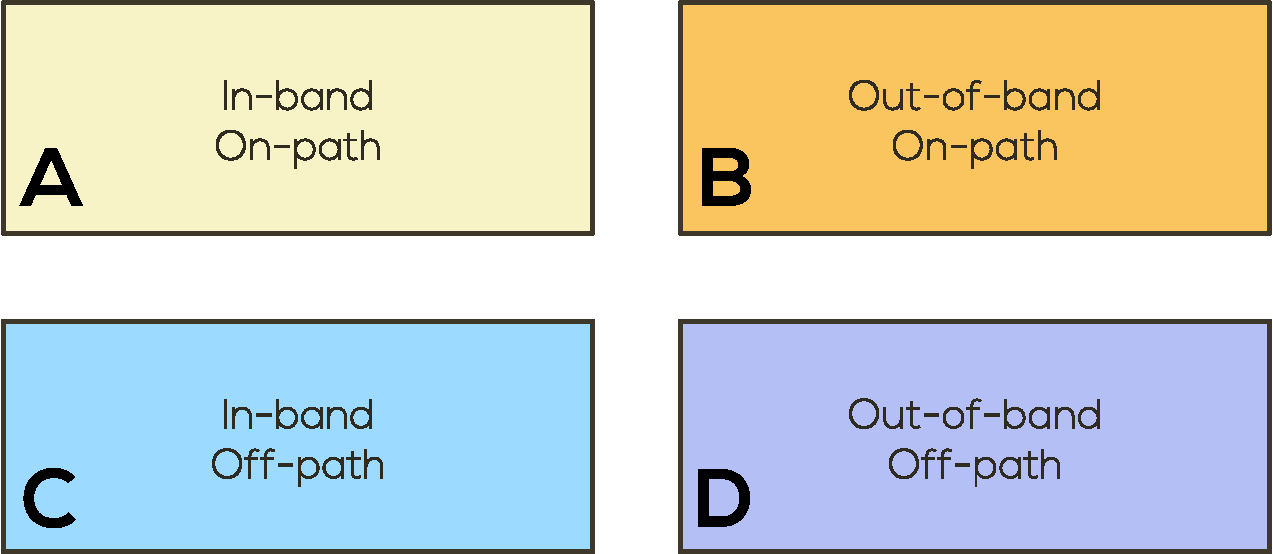
\includegraphics[width=0.9\textwidth]{chap4-fig-fw-outline}
\caption{Framework for classifying congestion control~\cite{Singh:PhDFw}.}
\label{fig:4:fw}
\end{figure}

A congestion control algorithm needs to pick one or more measurement point
(picking multiple adds to the feedback overhead) and then choose a method
to signal it to the sending endpoint. The algorithm can choose to report it in-band by
encapsulating the cues, either by piggybacking them on the endpoint's own media
packets as RTP header extensions (this adds to the header overhead of a media
packet) or as RTCP extension blocks (see section~\ref{fw.freq} for details on
feedback frequency). Or the congestion control algorithm can choose to signal
the cues out-of-band, i.e., re-use the signaling path (e.g., SIP, XMPP) or
setup an alternate signaling path (e.g., HTTP or websockets). THe following are
examples for each category in the framework:

\textbf{\texttt{A) In-path, In-band}}: The congestion control algorithm in
this case relies on the cues reported in an RTCP feedback from the receiver.
For example, TFRC using information in RTCP RR, TFRC using additional loss
reported by ECN markings, Temporary Maximum Media Stream Bit Rate Request
(TMMBR), Receiver Estimated Max Bit rate (REMB).

\textbf{\texttt{B) In-path, Out-of-band}}: The congestion control algorithm
relies on the cues reported in the signaling channel; for example, RTSP implements
a \emph{Speed} parameter to vary the transmission rate, or 3G base stations announce
the new rate when capacity changes due to cell-loading or handover.

% announcing bandwidth in the SDP at the start of the session (instead of
% starting at a low media bit rate) for rudimentary congestion control,

\textbf{\texttt{C) Off-path, In-band}}: The congestion control algorithm
relies on reports from multiple in-band sources; for example, in Multipath
RTP, congestion on one path causes a change in the fractional distribution of
traffic on each path.

\textbf{\texttt{D) Off-path, Out-of-band}}: The congestion control
algorithm relies on third party sources such as receiving bandwidth or
congestion notifications from congestion maps, bandwidth lookup services,
super-peers and overlays.

% monitoring: long-term, short-term

% Additionally if the cue reliably
% describes the onset of congestion (\emph{knee}) or the collapse
% (\emph{cliff}).

% \begin{figure}[!h]
% 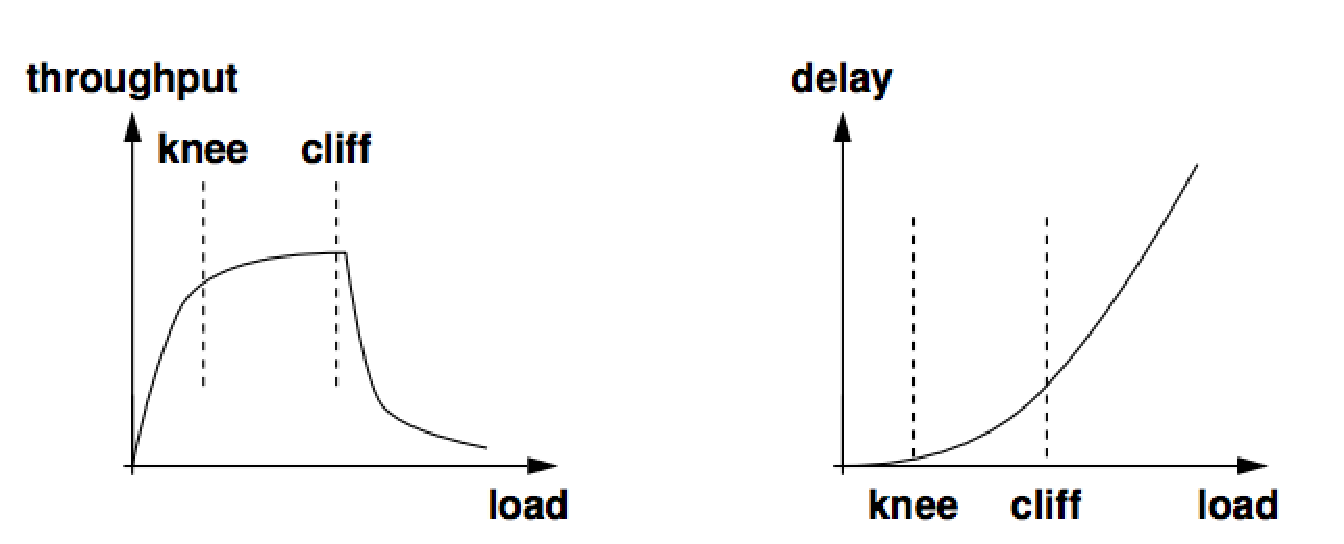
\includegraphics[width=\columnwidth]{chap4-knee-cliff}
% \caption{Shows the variation throughput and delay with increasing network load.}
% \label{fig:4:knee}
% \end{figure}

\section{Congestion Control Evaluation}
\label{fw.cc.eval}

% We need to define a set of requirements in order to design a congestion
% control algorithm for multimedia streams. Later these requirements are used as
% a checklist to evaluate the suitability of the proposed algorithms.

Real-time interactive communication differs greatly from \emph{elastic}
traffic because the sender generates media packets in real-time and expects it
to be delivered in hundreds of milliseconds, and the receiver consumes the media
packets almost immediately, hence late-arriving packets are useless.
Additionally, real-time communication systems are able to tolerate some amount
of packet loss and adapt the media rate over a fairly large range.
\cite{draft.rmcat.req} lists a set of requirements for RTP-based interactive
multimedia sessions; these requirements form the basis of the guidelines
described in~\cite{draft.rmcat.evaluate}. In~\cite{draft.rmcat.eval.test}, we
define a catalog of \emph{traffic flows} traversing through a \emph{network
topology} with varying \emph{link characteristics} and diverse \emph{queuing}
strategies. By picking one feature from each category, we
construct scenarios to evaluate the performance of the congestion control. The
evaluation scenarios are built using the following components: network
topology, link and router characteristics.

The difference between testing in real-world deployments and in simulations is
also important to consider, mainly in terms of the accuracy of RTT
measurements which impacts delay-based algorithms (e.g., TFRC). Time-slot-driven
simulation systems, such as \emph{ns-2}~\cite{ns2}, have accurate timing that
is not representative of real-world systems. Testbeds usually use
dummynet~\cite{Carbone:2010p3502}, NetEm~\cite{netem}, or packet traces to
emulate the variation in link capacity, latency, intermediate router queue
length, and packet losses. 

It is also possible to use actual machines placed at geographically distinct
locations and send media traffic between them; however, in this case, it is
not possible to run a controlled experiment anymore because of the varying
amount of cross-traffic generated by other hosts in the network.  Usually the
last step in the evaluation process involves deploying the congestion control
algorithm on several (thousands of) endpoints and showing that it behaves as
described without breaking anything on the network (i.e., causing a congestion
collapse).

\subsection{Network flows}

In this section, we describe typical test scenarios for evaluating congestion
control algorithms. These test scenarios are not supposed to be exhaustive
but show the applicability range of the algorithm.

\begin{enumerate}
\setlength{\itemsep}{0pt}

\item \textbf{\texttt{Single media flow on an end-to-end path}}: This scenario
describes the best case, wherein the network puts each flow identified by its
5-tuple (protocol, source and destination IP address, source and destination
port numbers) in its own queue, thus the flow using the proposed congestion
control algorithm does not encounter any cross-traffic.

\item \textbf{\texttt{Single media flow competing with multiple similar
flows}}: In this scenario, the flow using the proposed congestion control
algorithm competes with multiple flows using the same congestion control algorithm
(i.e., all flows are interactive multimedia).


\item \textbf{\texttt{Single media flow competing with multiple TCP flows }}:
In this scenario, the flow using the proposed congestion control algorithm
competes with TCP flows. These maybe \emph{short} TCP flows representing
common web-traffic patterns or \emph{long} TCP flows depicting bulk transfers
(e.g., large file downloads).

\end{enumerate}

% In Section~\ref{rg.title}, we describe the network traffic scenarios to
% evaluate the proposed congestion control algorithms, namely, when the flows
% are a) alone, b) competing with self-similar flows, and c) competing with TCP
% flows (short-, long-lived) on a bottleneck link.




\subsection{Link characteristics}

The link characteristics can be broken down into the following categories:
capacity, latency, and loss. The capacity of a link mainly varies in wireless
networks (for example in 3G, LTE, WLAN, etc). In Wireless LAN (WLAN) networks,
the capacity varies depending on the density of nodes using the network. The capacity in
mobile networks (e.g., 3G, LTE) fluctuates for each user because of fading,
interference, mobility, handover, cell loading, etc. The latency of a link
is measured as the propagation and serialization delay. Queuing delay is based on the
queue size of the router and hence, is a router characteristic. Latencies between
nodes typically vary from a few milliseconds to a few seconds. Commonly used
values are: LAN (very low delay, <1\,\emph{ms} ), low delay (<40\,\emph{ms}),
trans-continental (>100\,\emph{ms}), or satellite links (>500\,\emph{ms}).
Packet losses are modeled using the Gilbert-Elliott
Model~\cite{gilbert1960capacity, elliott1963estimates} or by packet
traces~\cite{ellis:2011:dataset, 3gppSim}.


\subsection{Router characteristics}

 % Queue-size and Queue type.

Apart from managing packet routing, a router also manages congestion; when a
packet arrives at a higher rate than it can be processed, the router queues the
packet. The routers then use \emph{priority queuing}, \emph{fair queuing}, or
\emph{weighted fair queuing (WFQ)}~\cite{rfc4594} to decide which traffic
class to transmit or drop packets from during congestion. When congestion
occurs within the same traffic class, the router discards packets using
\emph{tail drop}, \emph{Random Early Detection (RED)}~\cite{Floyd:RED}, or
\emph{Weighted Random Early Detection (WRED)}.

We describe the queue sizes as a function of time, i.e., it is the depth of
the queue or the amount of time the packet will remain in the queue before it
is discarded. However, in practice, the queue size is measured in number of
packets. We convert the queue depth (measured in time) to queue length (number
of packets, MTU is typically 1500 bytes) using:

\begin{equation*}
  \mathrm{QueueSize}_\mathrm{packets} = 
    \frac{\mathrm{QueueSize}_\mathrm{sec} \times
    \mathrm{Throughput}_\mathrm{bps}}{\mathrm{MTU} \times \mathrm{8}}
\end{equation*}

For example, a router with a throughput of 1\,\emph{Mbps} and a 1\,\emph{s} queue depth would be
capable of handling 83 packets (queue length). A 100\,\emph{ms}
queue depth may represent a short queue, while a 10\,\emph{s} queue depth represents
a buffer-bloated queue.

\subsection{Network topology}

We should run different types of network topologies to evaluate the
performance of congestion control. Depending on the amount of cross-traffic,
the bottleneck link will move from one node to another in the network. Also,
the bottleneck in each direction may be different due to the asymmetry of
access links. Additionally, the varying capacity of the access link (e.g., in
wireless environments) may be the bottleneck.


\begin{figure}
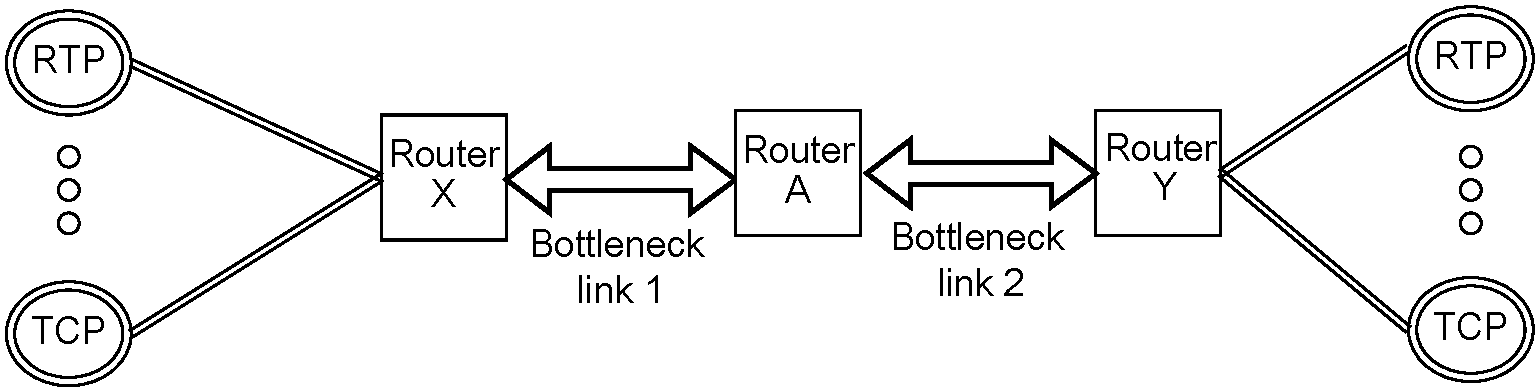
\includegraphics[width=\textwidth]{chap4_fig_sim_topology}
\caption{Typical network topology for evaluating congestion control consisting
of traffic flows (evaluating flow and cross traffic), links and routers.}
\label{fig:4:topology}
\end{figure}


Figure~\ref{fig:4:topology} shows an example of the evaluation setup. This
topology is commonly called the \emph{dumb-bell} topology. Another common
topology is \emph{parking lot}, which uses multiple bottlenecks instead of a
single bottleneck; however, both use common concepts.


To define a scenario, we need to choose the following: the type of cross-
traffic (self-similar, short- or long-lived TCP), the characteristics of the
cross traffic (e.g., duration), the characteristics of the edge routers
(Router X and Y) and the impairments in the network. Lastly, we have to
measure and analyze the performance of the multimedia system.


\subsection{Our Evaluation Setup}

Our research made use of the network simulator (\emph{ns-2})~\cite{ns2} or a
testbed made up of real-machines. The individual link characteristics in the
testbed were either controlled by NetEm~\cite{netem} or by
dummynet~\cite{Carbone:2010p3502}; the intermediate machines that ran
NetEm/Dummuynet ran kernels re-compiled at 1000Hz for better performance. The
endpoints typically ran stock Linux, such as Ubuntu 10.04 or 12.04. In some
cases, we used bandwidth and packet loss traces provided by
3GPP~\cite{s4.eval.bitrate} or collected them ourselves~\cite{sharmistha-thesis}. 
Additionally, we ran some tests between machines in Helsinki and the
Amazon data centers located in Virgina (US-EAST) and Ireland. The details of the
individual test scenarios are discussed in detail in the associated scientific 
papers.

\subsection{Metrics for Çongestion Control}
\label{subsec.metrics}

In this section, we introduce metrics for evaluating congestion control
algorithms. Multimedia application observe the congestion cues, and react to
the changes in the cues, by modifying the encoding/sending rate to match the
available end-to-end bit rate. The sender's goal is to minimize losses at the
receiver while maintaining a stable throughput. Losses are caused by
congestion or by  bit-errors and are detrimental to video quality. Although,
real-time communication is tolerant to a small amount of losses, bursty loss
should be avoided.  

% Bit-errors are due to the physical properties of the network and cannot be
% predicted ahead of time. Congestion losses are due to over-utilization of the
% links and may cause long delays or congestion-induced drops at the router.



\begin{figure}
\centering
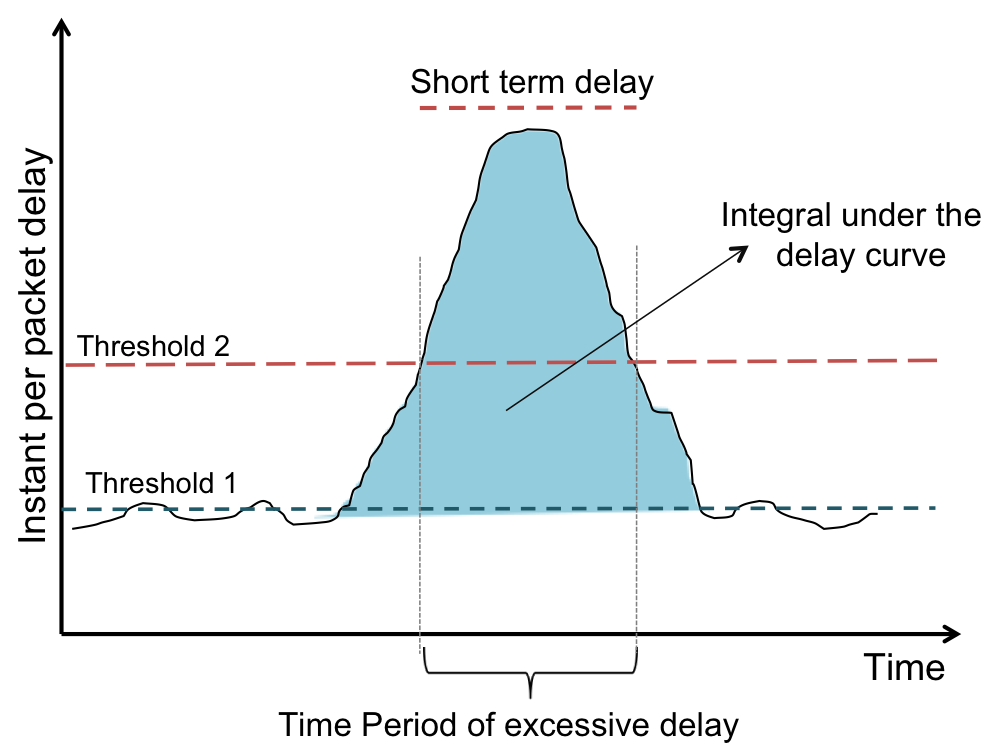
\includegraphics[width=0.75\textwidth]{chap4_fig-perf-metrics}
\caption{Metrics for congestion control.}
\label{fig:4:rc_model}
\end{figure}

Figure~\ref{fig:4:rc_model} schematically shows the instant per-packet delay
over time observed at the receiver. The sender reacts to the changes in the
available path bit rate. Exceeding the available path bit rate may lead to a
temporary increase in per-packet delay until the rate adaptation measures take
effect and, optionally, to packet losses if the queue capacity is exceeded.

For the delay, we define three values:
\begin{itemize}
\setlength{\itemsep}{0pt}

\item \textbf{\texttt{Threshold 1}} refers to the mean one-way delay observed
under normal operating conditions; this value may be defined statically
according to expectations for a certain environment, or determined
dynamically. This reflects the mouth-to-ear or camera-to-eye delay.

\item \textbf{\texttt{Threshold 2}} defines the maximum acceptable one-way
delay for a packet after which the rendering of the received media packet is
no longer meaningful. Packets arriving later than threshold 2 will be
discarded.

% Threshold 2 may be, e.g., 100-500ms for video, since the human eye
% is more tolerant to video glitches~\cite{s4.eval.fw}.

\item The \textbf{\texttt{short-term delay peak}} reflects the maximum delay
peak encountered during a congestion control operation. This may be either
caused by the appearance of cross-traffic on the bottleneck link or due to
congestion resulting in self-inflicted delay.

\end{itemize}

For losses, we consider two values:
\begin{itemize}
\setlength{\itemsep}{0pt}

\item \textbf{\texttt{Packets lost}} in the network due to bit errors and/or
increased queue lengths or overflows (e.g., caused by drop-tail or RED queue
management).

\item \textbf{\texttt{Packets discarded}} at the receiver because their
arrival delay violated threshold 2.

\end{itemize}

Additionally, we measure the instantaneous and average encoder rate, receiver
rate and goodput. The instantaneous rate is calculated at 1 second intervals. The
Average Bandwidth Utilization (ABU) is the ratio between the instantaneous
goodput (or encoding, receiving bit rate) and the instantaneous channel
capacity at 1 second intervals. An ABU larger than 100\,\% represents over-utilization 
and the duration over which it is over 100\,\% signifies the congestion period.


Peak Signal-to-Noise Ratio (PSNR) is the ratio between the maximum possible
power of a signal and the power of a noisy signal. The maximum power signal is
presumed to be the original signal, while the noisy signal is the received data
signal that has undergone the cycle of compression-transmission-decompression.
While PSNR is the most widely used objective video quality metric, it does not
perfectly correlate with perceived visual quality due to the non-linear
behavior of the human visual system~\cite{itu-t-j247}. Another criticism
against PSNR is that it does not incorporate time in its calculation. Despite
its shortcomings, we use PSNR as a yet another indicator for measuring the
performance of congestion control.

% It has been observed that the pictorial quality perceived by the human visual
% system is also affected by the overall general impression of the viewed video
% stream. In addition, recent studies have shown that human visual system awards
% higher response to more salient image locations and
% features~\cite{Li02asaliency, Ong:2006p3066}.


\section{Circuit Breakers for Unicast RTP Sessions}

If congestion control is not implemented by multimedia applications, they can
cause severe congestion in the network, especially if high data rate media
traffic is sent over low-capacity networks. This can not just disrupt the
multimedia's quality of experience but also other applications on the network.

We are developing a circuit breaker algorithm that can work with unmodified
RTP applications to determine when these non-adaptive multimedia
applications are causing excessive network congestion and force them to cease
transmission.  We envision that the congestion control algorithms for
multimedia standardized in the IETF will need to work inside the envelope of
this circuit breaker algorithm~\cite{draft.rmcat.evaluate}, i.e., a multimedia
application implementing congestion control should not trigger the circuit
breaker. Consequently, the circuit breakers cannot be too aggressive in
terminating media flows because it should allow sufficient time for the
congestion control algorithm to monitor and respond to congestion cues.

The circuit breaker algorithm in the short term will serve as a policer,
during which time the congestion control algorithm is developed. Developing
standard congestion control algorithms for unicast RTP-based interactive
multimedia applications is expected to be a multi-year process in the IETF.
Therefore, the development of the circuit breaker is on a tight schedule, to
be ready for inclusion in the initial roll-out of the WebRTC (Web-based 
Real-time Communication) framework~\cite{jennings:2013:webrtc} in web browsers.

\subsection{Circuit Breaker Design}
\label{fw.cb.design}

The RTP circuit breaker algorithm relies on the basic feedback mechanisms
defined in the RTP Control Protocol (RTCP)~\cite{rfc3550}. That is, it solely
uses the information available in the RTCP Sender Report (SR) and Receiver
Report (RR) packets to detect if the flow is overusing the capacity or causing
congestion.

The congestion indicators considered for implementing circuit breakers are: 1)
the network \emph{round trip time} (RTT) calculated  using timing information
in RTCP SR and RR packets, 2) the \emph{jitter} estimated by the receiver over the
last reporting interval, and 3) \emph{fractional packet loss} and \emph{cumulative
loss} reported by the receiver during the last RTCP interval. These
indicators  unfortunately only provide a limited insight into the behavior of
the network and cannot be used as strong signals for a circuit breaker.

Variation in RTT is used as a congestion indicator in delay-based congestion
control algorithms. Additionally, some algorithms use RTT estimates to
configure connection timeouts. In RTP/RTCP, the RTT is estimated infrequently
because the feedback intervals are rather long, making it difficult to detect
the cause in variation of delay. Likewise, variation in jitter can indicate a
transient network congestion but does not provide a strong enough signal to implement
a circuit breaker. On the other hand, loss is a strong indicator of congestion
in networks where packet losses predominantly occur due to queue overflows, and
is a less accurate indicator where packet loss occurs due to bit-error
corruption (e.g., wireless and mobile links). Therefore, we base the circuit
breaker conditions on packet losses. 

\begin{enumerate}
\setlength{\itemsep}{0pt}

\item \textbf{\texttt{Media Timeout}}: An endpoint is sending media data but when
the receiver reports a non-increasing \emph{Highest Sequence Number} (HSN) for
two consecutive RTCP intervals, the flow is terminated.

\item \textbf{\texttt{RTCP Timeout}}: An endpoint is sending media data but if it
receives no RTCP RR for three consecutive RTCP intervals, the flow is
terminated.

\item \textbf{\texttt{Congestion}}: An endpoint is sending media data and if it
receives RTCP RRs indicating fractional packet loss, it calculates the TCP-friendly 
rate and compares it to the sending rate. If the sending rate exceeds
the TCP-friendly rate  by a factor of 10 for two consecutive RTCP intervals,
the flow is terminated.

\end{enumerate}

Full details of the RTP circuit breaker algorithm is specified
in~\cite{draft.rtp.cb}, which is a work in progress and covers various
deployment cases such as multiple media sources, impact of shorter-than-standard 
reporting interval, deployment of Explicit Congestion Notification
(ECN), etc.

In \citepub{c:cb}, we apply these circuit breaker conditions to non-adaptive
RTP media flows deployed on ADSL and cable modem links.  Such flows typically
do not implement congestion control at this time, and are likely to cause
congestion if deployed on the Internet. We carried out a series of experiments
based on real-world traces and on a testbed emulating real-world conditions.
Our results show that the proposed RTP circuit breaker performs well,
triggering in cases of bursty loss and in sessions that are congesting the
links, and does not trigger in low-loss and non-bursty scenarios.


\begin{figure}
  \centering{
    \subfloat[Non-bursty]{
      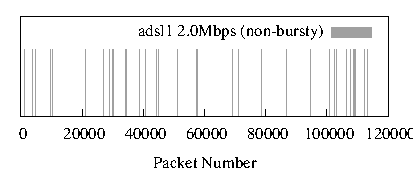
\includegraphics[width=0.66\textwidth]
      {chap4_graph_cb_20090707-1515-barcode}
    } \\
    \subfloat[Bursty]{
      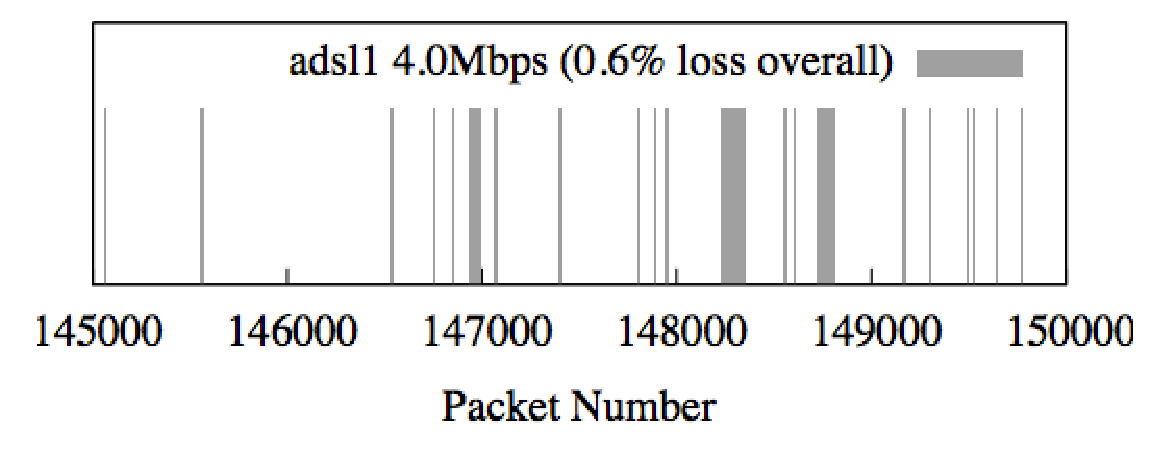
\includegraphics[width=0.66\textwidth]
      {chap4_graph_cb_bursty}
    }
  }
  \caption{Sample non-bursty (a) and bursty (b) packet loss traces.
  The bursty packet triggers the circuit breaker even though the overall
  packet loss ratio is 0.6\,\%.}
  \label{fig:4:bursty}
\end{figure}

\begin{table}
  \begin{center}
    \begin{tabular}{rcc}
    \toprule
      \textbf{Loss Pattern}   & \textbf{Triggered} & \textbf{Did not trigger} \\
    \midrule
             Loss free &   0.0\,\% & 100.0\,\% \\
       Non-bursty loss &   0.0\,\% & 100.0\,\% \\
          Bursty loss  &  11.9\,\% &  88.1\,\% \\
    \bottomrule
    \end{tabular}
    \caption{Sessions triggering the circuit breaker by loss pattern.}
    \label{tab:4:cb_bursty}
  \end{center}
\end{table}

We simulated the RTP circuit breaker performance on $3833$ generated RTCP traces
corresponding to the measurements collected in \emph{dataset-A} and
\emph{dataset-B} of~\cite{ellis:2011:dataset}. Of these, $1626$ traces have no
packet loss, and hence cannot trigger the RTP circuit breaker. The remaining
traces each include at least one lost packet. We categorize the remaining
traces into two categories: those that have non-bursty packet loss, and those
that exhibit bursty loss using the definition of bursty loss
from~\cite{rfc3611} (Figure~\ref{fig:4:bursty} shows representative samples of
the non-bursty and bursty packet loss patterns). The data comprises $1344$
traces with bursty loss and $863$ traces with non-bursty loss.



Table~\ref{tab:4:cb_bursty} shows the fraction of sessions that triggered the
RTP circuit breaker for each of the categories of packet loss. The RTP circuit
breaker did not trigger for sessions without loss; it also did not trigger for
any of the sessions with non-bursty packet loss. However, we observe that the
RTP circuit breaker is triggered more often in sessions that contain bursty
packet loss. 

\begin{figure}[!t]
  \centerline{
    {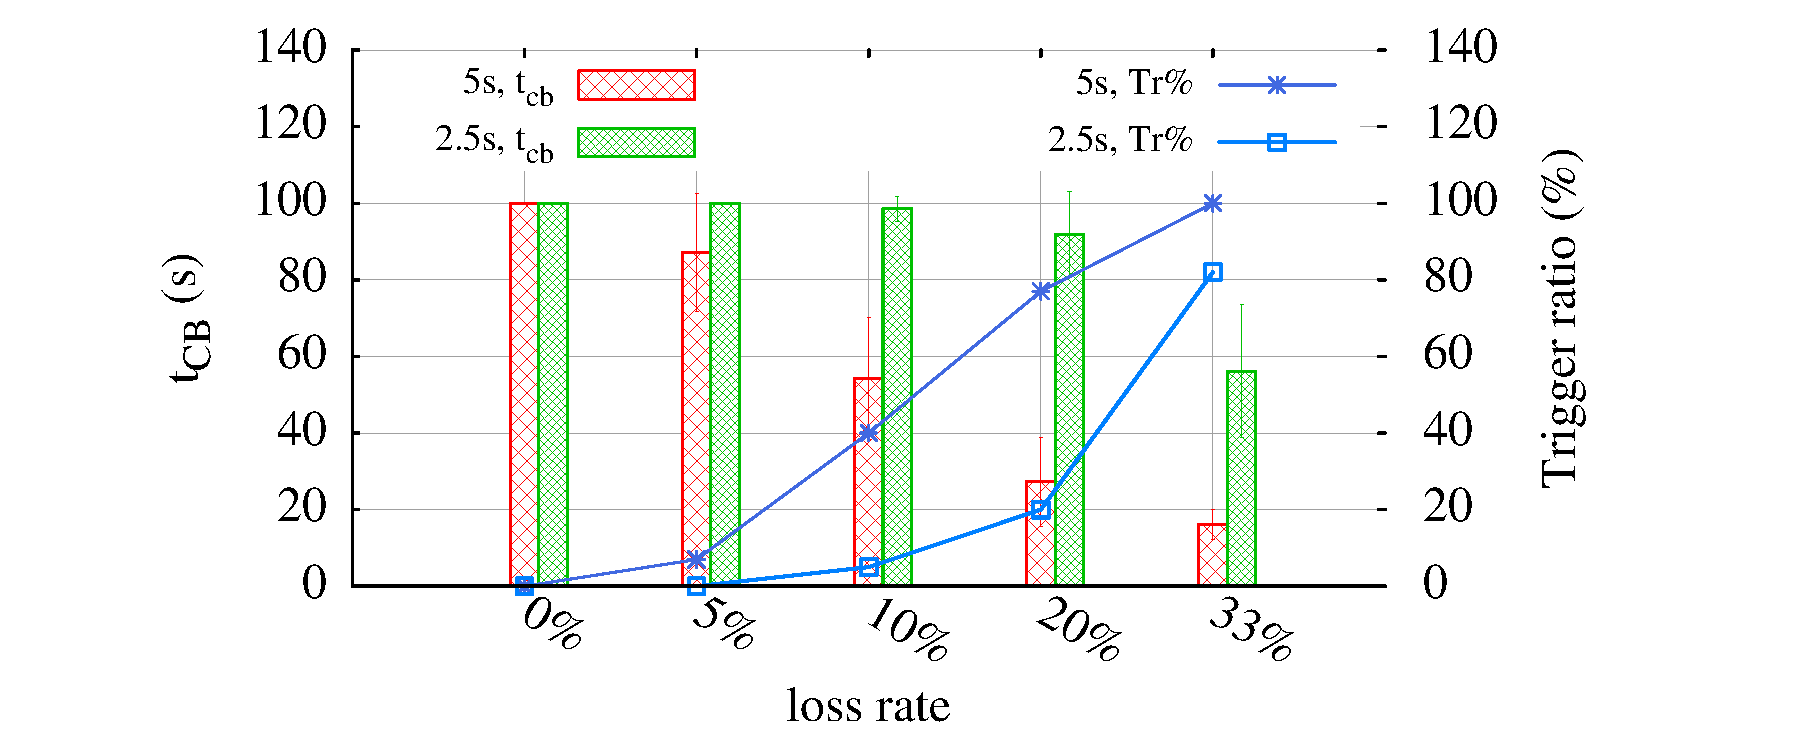
\includegraphics[width=\textwidth]{chap4_graph_cb_cmp_trr_2s}}
  }
  \caption{Impact of using a shorter RTCP interval on the
  circuit breaker. Each scenario was run 50 times and the error bars represent
  the 95\,\% confidence level.}
  \label{fig:4:short-rtcp}
\end{figure}

The circuit breaker conditions trigger mainly due to loss. Figure~\ref{fig:4:short-rtcp} 
shows that the percentage of sessions triggering the circuit breaker
increases with the increase in loss rate. The figure also shows the impact of
the RTCP reporting interval, i.e., by reducing the RTCP interval from 5\,\emph{s} to
2.5\,\emph{s}, fewer sessions are terminated. The endpoints become robust to loss of
feedback packets by sending feedback often and we observe a longer time for
triggering the circuit breaker ($t_{CB}$).

\subsection{Discussion about TCP throughput equations}

In Section~\ref{fw.cb.design}, we described the circuit breaker triggers when
the sending rate exceeds the estimated TCP throughput by a factor of 10. We
can estimate the TCP throughput either using Padhye's full TCP throughput
equation~\cite{padhye1998modeling} or using Mathis's simplified TCP throughput
equation~\cite{mathis1997macroscopic}.

In~\cite{padhye1998modeling}, Padhye \emph{et al.} show that the TCP
throughput for a long-lived TCP Reno connection can be estimated using the
following equation:
\begin{align*}
X_{Kbps} = &\frac{8 \times s}{R \times \sqrt{\frac{2*b*p}{3}}+t_{RTO} \times (3 \times \sqrt{\frac{3*b*p}{8}})\times p \times (1+32 \times p^2)}\\
\end{align*}
While Mathis \emph{et al.} in \cite{mathis1997macroscopic} show that under
conditions of low packet loss, Padhye's equation can be simplified to:
\begin{align*}
    X_{Kbps} = & \frac{8 \times s}{R \times \sqrt{\frac{p \times 2}{3})}}
\end{align*}
\begin{itemize}
\setlength{\itemsep}{0pt}
{\footnotesize
\item[] \texttt{X is the transmit rate in Kbps.}
\item[] \texttt{s is the average packet size in bytes.} 
\item[] \texttt{R is the round trip time in seconds. }
\item[] \texttt{p is the loss event rate, $\forall p \in [0.0, \cdots ,1.0]$.}
\item[] \texttt{$t_{RTO}$ is the TCP retransmission timeout value in seconds, usually set to $\mathbf{4 \times R}$.}
\item[] \texttt{b is the number of acknoweldged packets in TCP; typically set $\mathbf{b=1}$.}
}
\end{itemize}
Mathis \emph{et al.} also show that the simplified TCP equation approximates
Padhye's full equation with reasonable accuracy~\cite{mathis1997macroscopic} .


In \citepub{c:cb}, our experiments on residential networks shows that the
simplified TCP throughput equation performs effectively, while using Padhye's
full TCP equation triggers the circuit breaker earlier. The data show that
the full TCP equation tends to be more sensitive to packet loss. In LTE
networks with a combination of a low RTT and high packet loss rate (due to
AQM), the circuit breaker using the simplified TCP throughput equation
does not trigger at all~\cite{Sarker:CB.lte}. However, using the Padhye's full TCP
throughput equation in these cases gives better
performance~\cite{Sarker:CB.lte}. We believe some of this over-sensitivity is
due to averaging packet loss events over long RTCP reporting intervals and the
fact that the RTT is estimated only once in that interval.

Overall, our preliminary results derived from experiments in a testbed,
and simulations based on real-world traces show that
the proposed RTP circuit breaker performs as intended, triggering in the case
of bursty  packet loss and  not triggering in the low-loss and non-bursty
scenarios. 

% The current analysis is based on measurements done in the UK and
% Finland, while these measurements may be representative of residential links
% in Europe, the infrastructure is likely to differ significantly in other parts
% of the world. Therefore, a wider measurement study of the RTP circuit breakers
% would be desirable.


\section{Summary}

In this chapter, we aimed to classify congestion control cues for real-time
communication based on: \emph{where they are measured?} (by in-path or  off-
path sources) and \emph{how they are reported?} (via in-band or out-of-band
signaling). We also describe other fundamental choices needed to implement
congestion control: congestion cues, reporting frequency and  circuit-breaker
conditions. Additionally, we describe a basic evaluation suite for measuring
the performance of any proposed multimedia congestion control algorithm;
derivatives of these test scenarios are used to discuss the performance of
congestion control in this thesis.

We specified the circuit breaker algorithm and discuss the performance of the
circuit breaker applied to non-adaptive multimedia traffic. Our results show
that it works as intended, i.e., it provides enough time for a congestion
control algorithm to respond to congestion cues before triggering the circuit
breaker. We also show that the endpoint can slightly vary the sensitivity of
the circuit breaker by choosing between the full and simplified TCP throughput
equation. In the forthcoming chapters, we discuss our proposals for congestion
control in various environments, several of which work within the constraints
imposed by the circuit breaker algorithm.




\chapter{Congestion Control for Interactive Multimedia}
\label{chap:cc}
Figure~\ref{fig:4:fw} in Chapter~\ref{chap:cc.fw} shows the structure of the
congestion control framework described in this thesis. The framework
categorizes \emph{in-path} sources and \emph{in-band} signaling for
implementing congestion control (corresponds to \emph{Block A} in
Figure~\ref{fig:4:fw}), which are discussed in this chapter. This chapter is
based on our work on congestion control for interactive multimedia
applications, which is documented in \citepub{c:3grc}, \citepub{c:hetrc},
\citepub{c:eval}, \cite{rfc7097},
\cite{draft.xr.bytes.discarded}, \cite{singh:2010.thesis} and
\cite{Singh:control.loops.api}.

In \citepub{c:3grc}, we propose a new congestion control algorithm for the
mobile (e.g., 3G) environment, to be deployed in the IP Multimedia System
(IMS). The main distinction between mobile (e.g., 3G, LTE) and other wireless
environments (e.g., 802.11x) is that the media streams are transmitted using
the \emph{unacknowledged mode}; the packets corrupted due to bit-errors (e.g.,
wireless interference) are not re-transmitted. Hence, the packets incur low
delay, compared to Wireless LAN where corrupted packets are retransmitted by
the link layer. We propose a sender-driven and a receiver-driven congestion
control, and evaluate the performance of the proposed congestion control
algorithm in a simulated environment (in ns-2) using real-world 3G
traces~\cite{s4.eval.bitrate, 3gppSim}. In \citepub{c:hetrc}, we extend the
approach in \citepub{c:3grc} for deployment on the Internet and show that the
congestion control scheme is deployable there as well. In \cite{rfc7097} and
\cite{draft.xr.bytes.discarded}, we propose RTCP XR block extensions that
indicate the number of bytes discarded and run-length encoding of discarded
packets, respectively. These packets are discarded by the receiver because
they arrived too early or too late to be played out by the receiver. This
information is used as a congestion cue by the sender.

% \cite{Singh:control.loops.api} discusses the application and API requirements
% for interactive multimedia congestion control. It describes the two control
% loops: a) between the receiver and the sender, and b) between the media
% encoder and the sending agent. In the first loop, the receiver notifies the
% sender about the current network characteristics. In the second loop, the
% sending agent requests a new media bit rate, and the encoder tries at best to
% meet it, sometimes under-shooting or over-shooting the requested rate.

Lastly, in \citepub{c:eval} we evaluate the performance of a congestion
control algorithm proposed by Google for WebRTC. We evaluate the performance
in diverse scenarios measuring scalability (\emph{how quickly is the
congestion control able to utilize the available capacity}), self-fairness and
competing against bursty cross-traffic. We evaluate the performance of
web browsers implementing the congestion control algorithm in our testbed that
emulates the diverse scenarios.

\section{Schemes of Congestion Control}

The congestion control algorithm can be implemented at the sender, at the
receiver, or the sender and receiver can operate co-operatively. The
\emph{sender-driven} scheme requires that the receiver measures the current
network condition and signals the observed congestion cues to the sender, which
calculates the sender's estimate and uses it as the new sending rate. In the
\emph{receiver-driven} scheme, the receiver calculates the new sending rate
(receiver's estimate) based on the observed congestion cues, and signals the
new rate to the sender, which, on receiving the new rate, adapts the media bit
rate to the received value. The \emph{co-operative} scheme is an extension to the
\emph{sender-driven} scheme. In this case, the receiver calculates the
receiver's estimated rate and signals it along with the observed congestion
cues; the sender at its end calculates its own estimate based on the
congestion cues and chooses a new sending rate, typically a value in between the
sender's estimate and the receiver's estimate. Figure~\ref{fig:cc:scheme}
shows the interaction of the sender and receiver for each scheme. The figure
merely shows the media flow in one direction; however, it should be noted that
the media in the simulation and the emulated testbed actually flow in both
directions unless explicitly mentioned. This is mainly done for the
convenience of representation and followed throughout the remainder of the
thesis.

\subsection{Sender-driven Congestion Control Schemes}

\begin{figure}[!t]
  \centerline{
    \subfloat[Sender-driven Scheme]{
      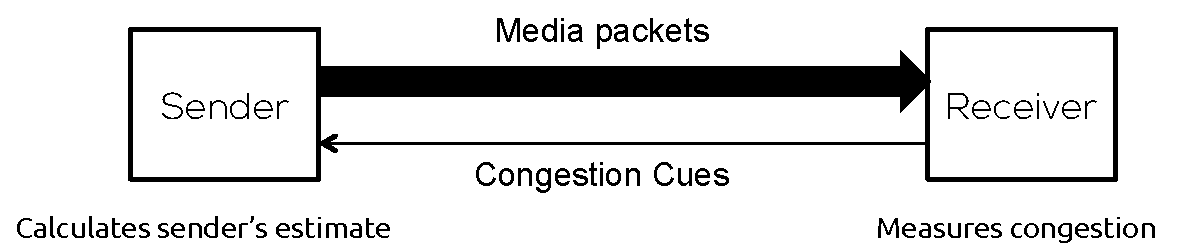
\includegraphics[width=0.9\textwidth]
      {chap5-fig-cc-scheme-s}
    }
  }
  \centerline{
    \subfloat[Receiver-driven Scheme]{
      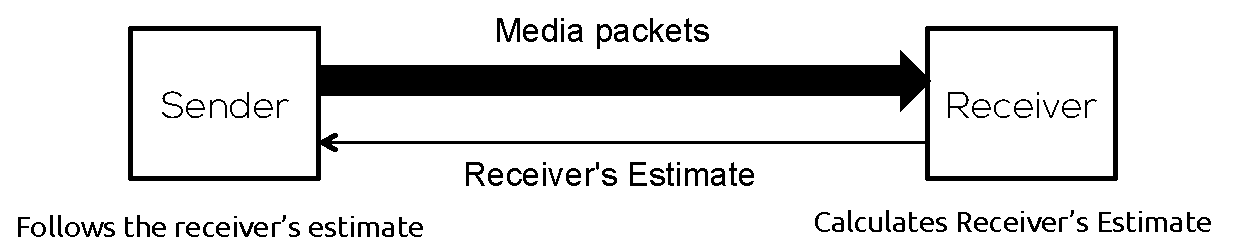
\includegraphics[width=0.9\textwidth]
      {chap5-fig-cc-scheme-r}
    }
  }
  \centerline{
    \subfloat[Co-operative Scheme]{
      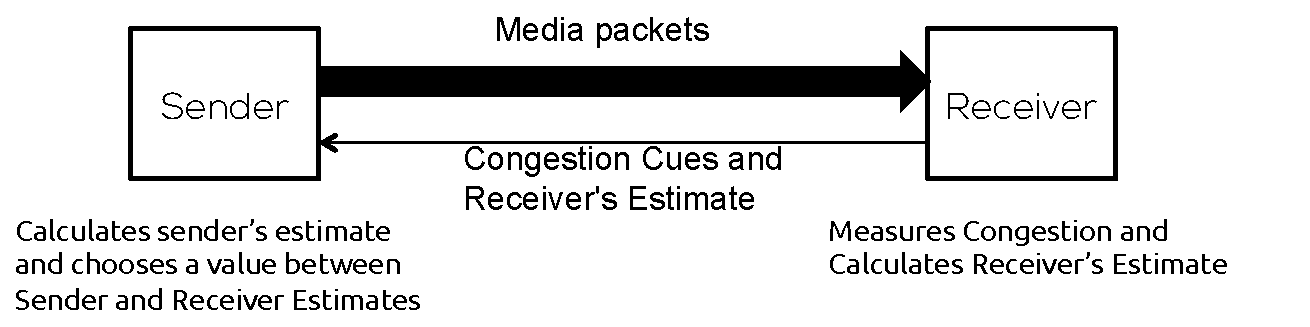
\includegraphics[width=0.9\textwidth]
      {chap5-fig-cc-scheme-c}
    }
  }
  \caption{Congestion control schemes: a) sender-driven, b) receiver-driven
and c) co-operative.}
  \label{fig:cc:scheme}
\end{figure}

TCP Friendly Rate Control (TFRC) is an equation-based congestion control
algorithm implemented at the sender~\cite{tfrc_347397} and is also implemented
as a profile~\cite{rfc4342} in the Datagram Congestion Control Protocol
(DCCP)~\cite{rfc4340}. TFRC uses the average packet size, round trip time
($RTT$), and loss ratio ($p$)~\cite{rfc3448} to calculate the new sending rate.
Formally, the sending rate in TFRC is calculated as follows:

\begin{align*}
 TFRC = &\; \frac{8 \times avg\_packet\_size}
{R \times \sqrt[]{\frac{2 \times b \times p}{3}} + t_{RTO} \times 
\left( 3 \times \sqrt[]{\frac{3 \times b \times p}{8}}\right) \times p \times
\left( 1+32 \times p^2 \right)}\\
where,\; b = &\; 1\\
t_{RTO} = &\; 4 \times R
\end{align*}

TFRC cannot directly be applied to RTP because TFRC requires per-packet
feedback, and in RTP, the RTCP feedback is not necessarily sent that
often~\cite{draft.rmcat.feedback}. Therefore, \cite{draft.rtp.tfrc} maps the
TFRC timing rules defined in~\cite{rfc4828, rfc5348} to that of the RTP/RTCP
feedback loop. It also proposes extensions to the timing rules in the
AVPF-profile~\cite{rfc4585} for very short RTTs ($<20ms$).
\cite{Gharai06:ICME} and \cite{VladBalan:2007dq} show that TFRC is stable on
paths with longer RTTs than those with smaller RTTs, but it too exhibits
saw-tooth behavior~\cite{saurin:2006:thesis}. Any algorithm that consistently
produces a sawtooth media rate is not well suited for real-time communication
because it generates a poor user-experience~\cite{Gharai:2002wt,
Zink03subjectiveimpression}.

Other sender-driven congestion control algorithms that we explored include the
Rate Adaption Protocol (RAP)~\cite{rap:752152} that uses a windowed approach which 
exhibits a sawtooth-type of behaviour. Zhu~\textit{et
al.}~\cite{rmcat-nada} use Pre-Congestion Notification (PCN), Explicit
Congestion Notification (ECN) and loss rate to get an accurate delay
estimate for implementing congestion control. In this case, they assume all
packets marked by ECN and PCN as lost. Their algorithm as specified now, 
relies on accurate measurement of one-way delay relying on clock synchronization.
Instead of just relying on RTT and loss for congestion control, 
Garudadri~\textit{et al.}~\cite{4397059} also use the
receiver playout buffer to detect the link utilization, i.e., the variation in the 
receiver playout buffer occupancy indicates an increase or decrease in congestion.
O'Hanlon~\textit{et al.}~\cite{rmcat-dflow} propose using a delay-based
estimate when competing with similar traffic and, using a windowed-approach
when competing with TCP-type cross traffic, they switch modes by applying a
threshold on the observed end-to-end delay. The idea is similar to the one
discussed in~\cite{budzisz2011fair}.




\subsection{Receiver-driven Congestion Control Schemes}

In receiver-driven congestion control, the receiver estimates the rate and
notifies the sender about the new sending rate. Temporary Maximum Media 
Bit-rate Request (TMMBR) is defined as a codec control message in \cite{rfc5104}.
It is generated by the receiver in a point-to-point video call. The receiver
calculates the new estimate (available capacity) based on the average 
inter-arrival time of RTP packets (\emph{video frames}). When the inter-arrival time
of the video frames increases beyond the expected arrival time in an observed
period, the receiver senses \emph{over utilization}. When the frames arrive early, the
receiver senses \emph{under utilization}. The receiver ignores the congestion event 
if it occur on short timescales and when receiving I-frames. 
The I-frames are large frames because they are spatially compressed and
are not temporally correlated to previous frames. Hence, these I-frames are
expected to cause queuing delay. The receiver, on detecting link over
or under utilization, modifies the \emph{receiver's capacity estimate}. 
The receiver sends the TMMBR message to the sender
indicating the maximum sending rate. Currently, interactive multimedia sessions
in 3GPP~\cite{3gpp.26.114} use TMMBR messages to notify the sender of the
expected sending rate. In WebRTC~\cite{jennings:2013:webrtc}, TMMBR is
expected to be used initially, before RTP congestion control is standardized
by the IETF~\cite{rtp-usage}. The expectation is that different WebRTC clients
may develop proprietary receiver-driven algorithms and use TMMBR as the
standardized mechanism to communicate the capacity estimate to the sender,
which will blindly follow it.


\subsection{Co-operative Congestion Control Schemes}
\label{cc:co-op}

The Next Application Data Unit (NADU)~\cite{nadu.1070341,nadu.1530486} is designed
for rate adaptation for video streaming in 3GPP~\cite{3gpp.26.234}. A NADU
receiver measures the playout delay (as a measure of buffer occupancy in time)
and signals it to the sender along with the next sequence number to be played
out. Conversational NADU (C-NADU) is an extension of NADU for congestion
control for interactive multimedia and is described in \citepub{c:3grc} and
\citepub{c:hetrc}. In C-NADU, the receiver also calculates the
\emph{receiver's capacity estimate} by measuring the frame inter-arrival time
and signals that along with the NADU report. If the video frame arrives at the
expected time, the receiver assumes no ongoing congestion, and if it arrives
later than the expected time, the frame is considered late and the receiver
diagnoses congestion. If the frame is delayed and misses its playout time, it
is discarded and in this case the receiver estimates congestion. Based on the
above cases, the receiver estimates the current capacity and signals it to the
sender. At the sender, the C-NADU controller calculates the TCP-friendly rate,
measures the variation in RTT ($75$ and $90$ percentile values) and calculates
the fraction of video frames that missed their playout deadline. Based on
these congestion cues and the receiver estimate, the sender chooses a new
sending rate.


Receiver-side Real-Time Congestion Control (RRTCC) is described in
\cite{draft.rrtcc} and is proposed as one of the solution candidates for
WebRTC by Google. Like C-NADU, RRTCC also has a receiver- and sender-side
component. The receiver-side measures the under or over utilization by
monitoring the timestamp jitter of the incoming frames. The arrival times are
modeled as a white Gaussian process. When the mean is 0 there is no
congestion; the mean is expected to increase when there is ongoing congestion
and expected to decrease when the congestion abates. Based on this
expectation, the receiver calculates the capacity estimate and signals it to
the sender. The sender calculates its estimate based on TFRC, and finally,
chooses the new sending rate as a value between the TFRC rate calculated by
the sender and the receiver's estimate. Full details of the algorithm proposed by
Google are documented in an Internet-Draft~\cite{draft.rrtcc}.



\begin{figure}[!t]
  \centerline{
    \subfloat[TFRC]{
      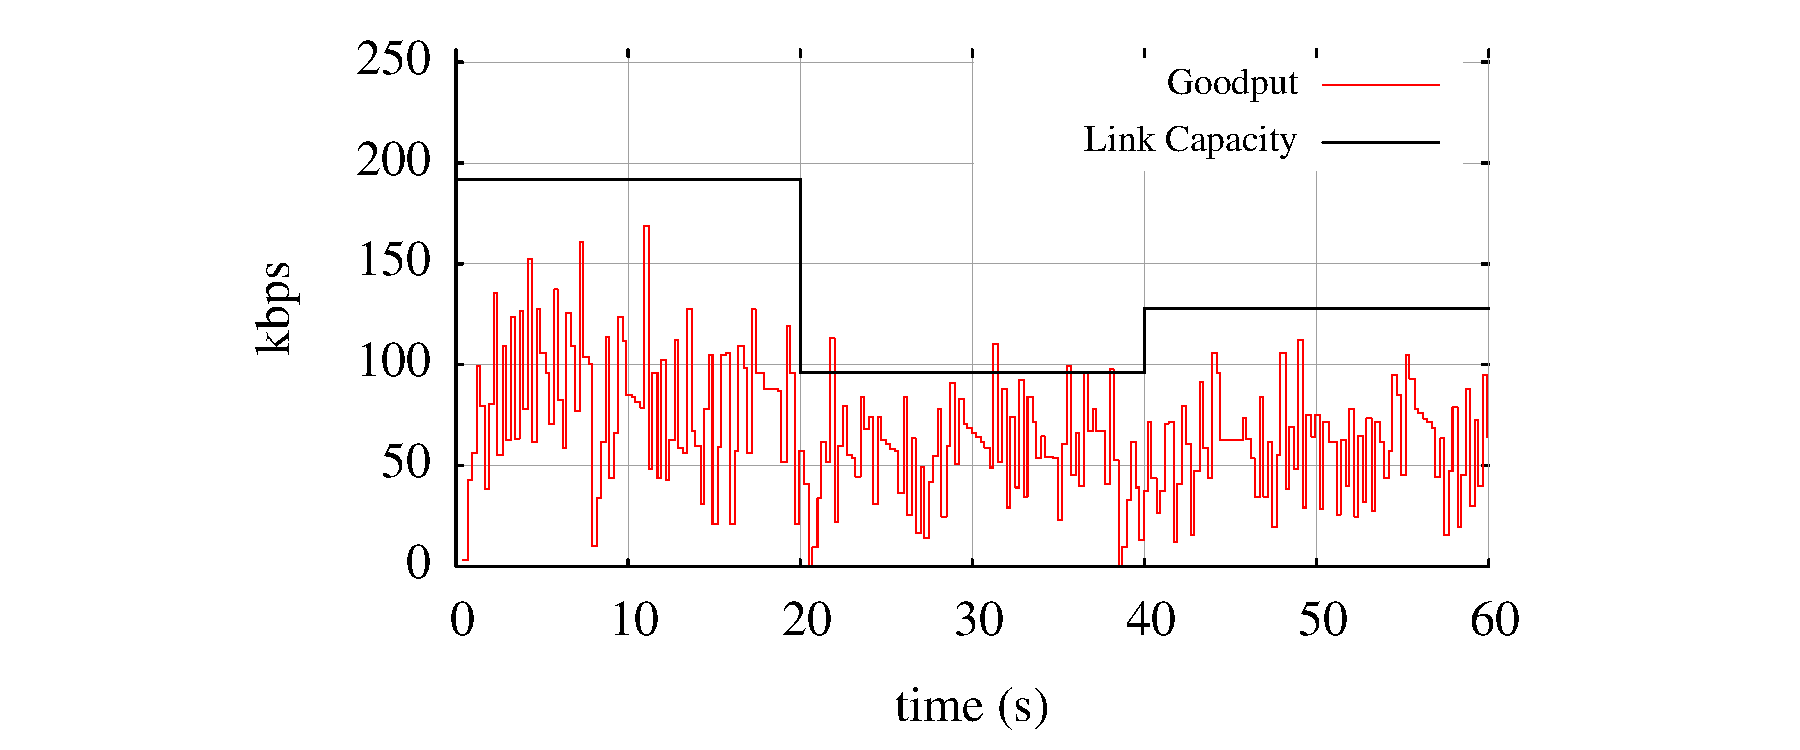
\includegraphics[width=0.5\textwidth, clip=true, trim=3cm 0 4.5cm 0]
      {chap5_graph_sl_tfrc}
    }
    \subfloat[TFRC]{
      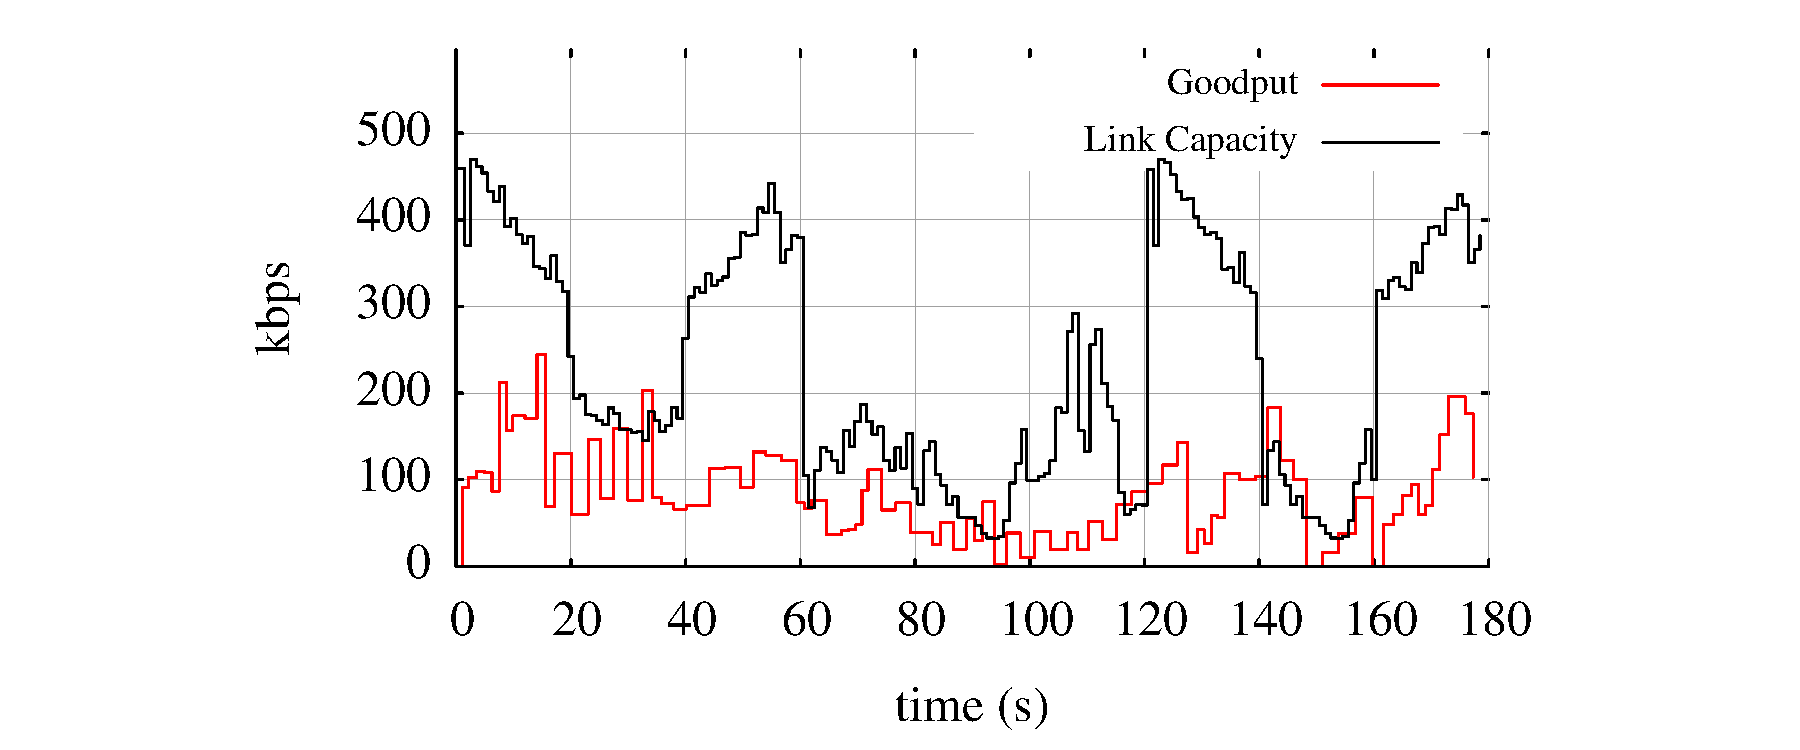
\includegraphics[width=0.5\textwidth, clip=true, trim=3cm 0 4.5cm 0]
      {chap5_graph_3g_tfrc_1}
    }
  }
  \centerline{
    \subfloat[TMMBR]{
      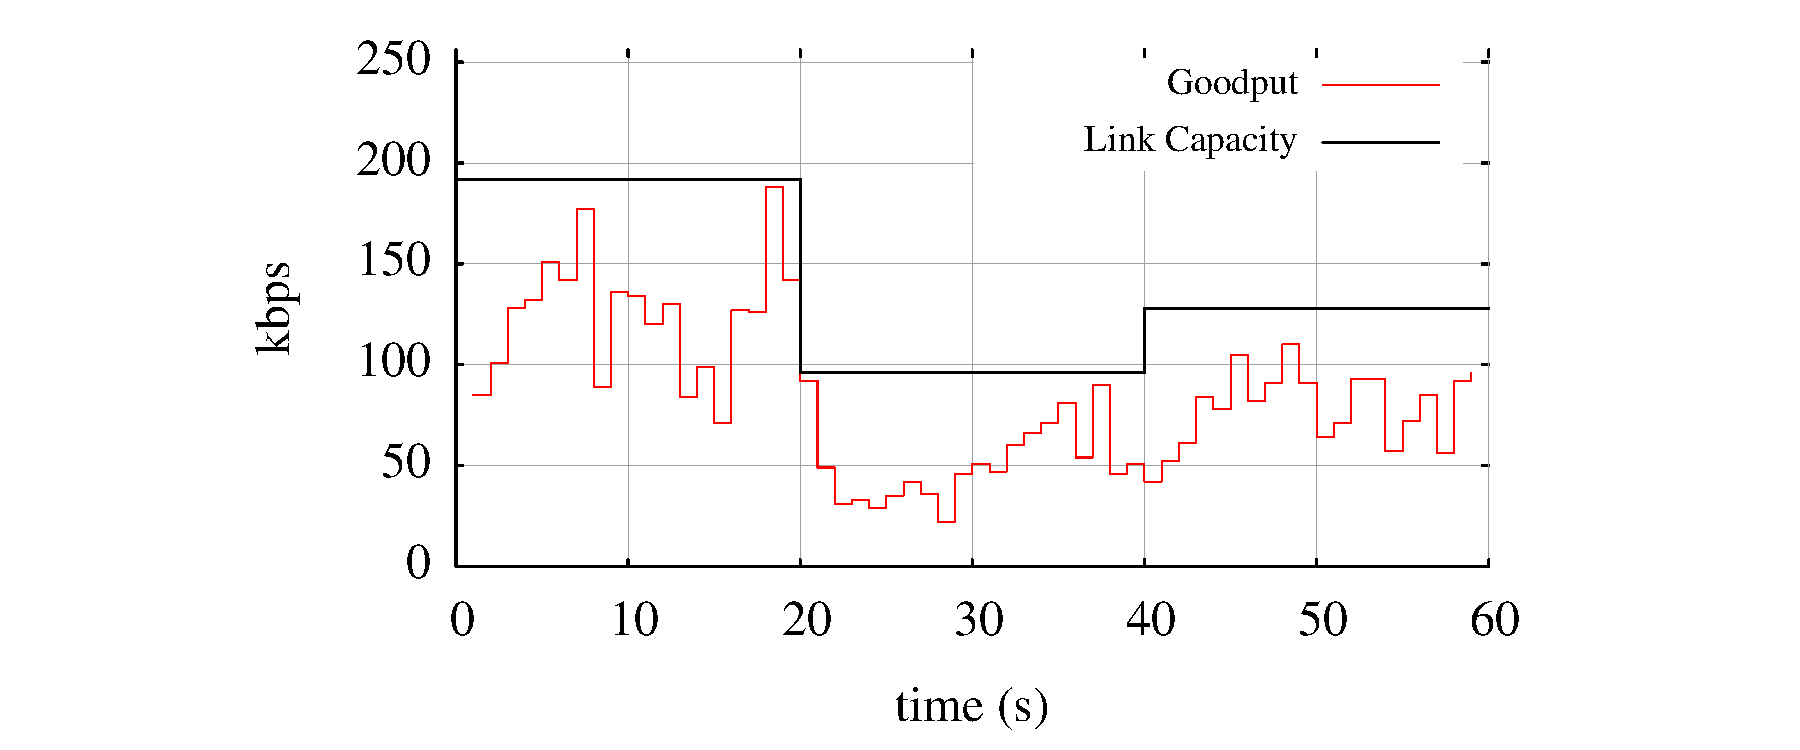
\includegraphics[width=0.5\textwidth, clip=true, trim=3cm 0 4.5cm 0]
      {chap5_graph_sl_tmmbr}
    }
    \subfloat[TMMBR]{
      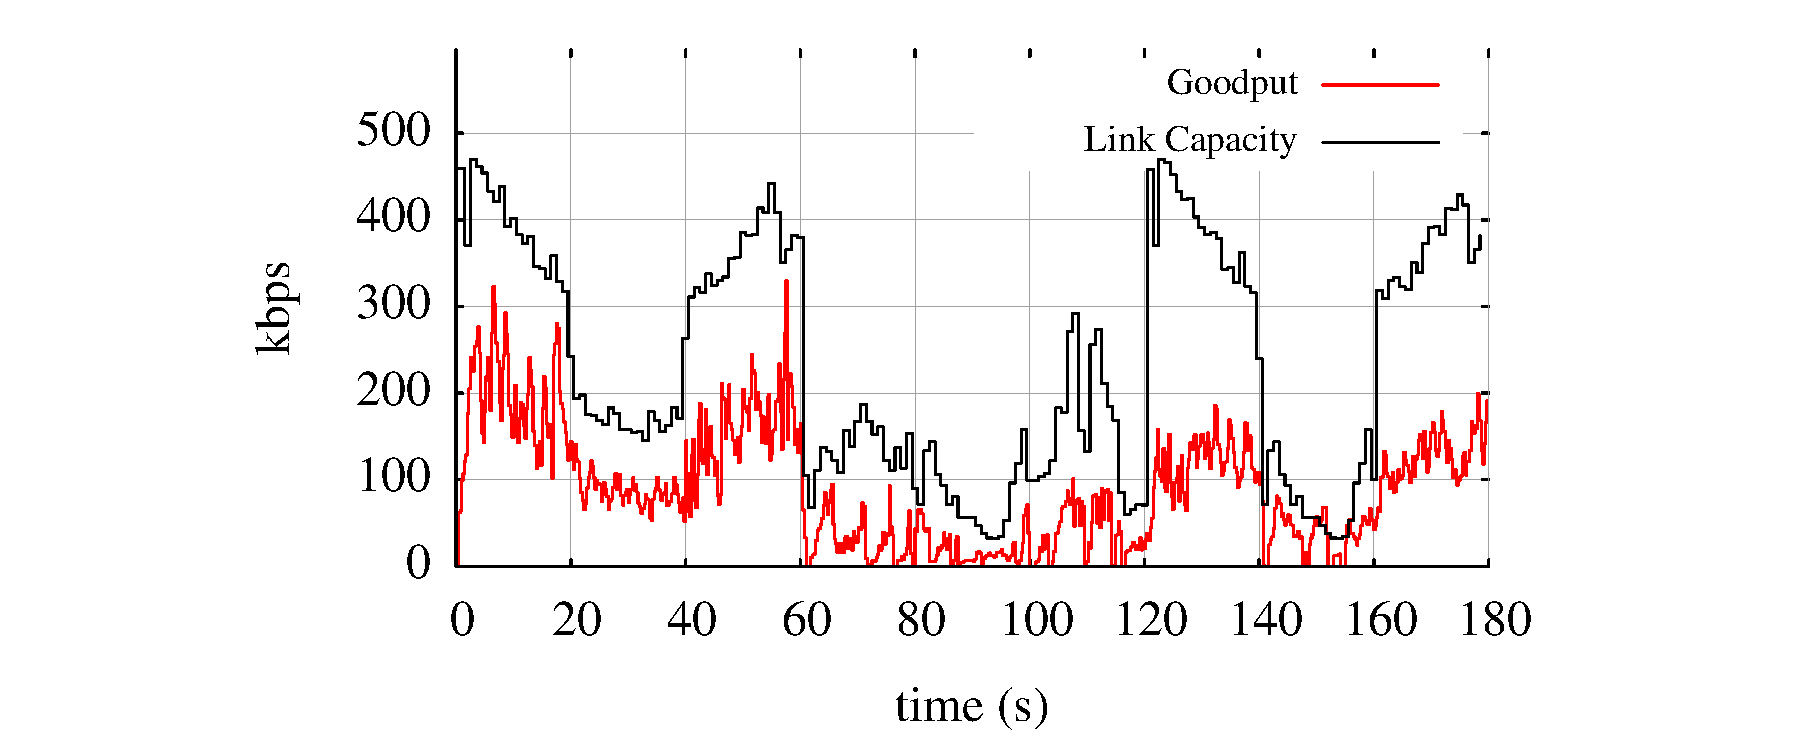
\includegraphics[width=0.5\textwidth, clip=true, trim=3cm 0 4.5cm 0]
      {chap5_graph_3g_tmmbr_u}
    }
  }
  \centerline{
    \subfloat[C-NADU]{
      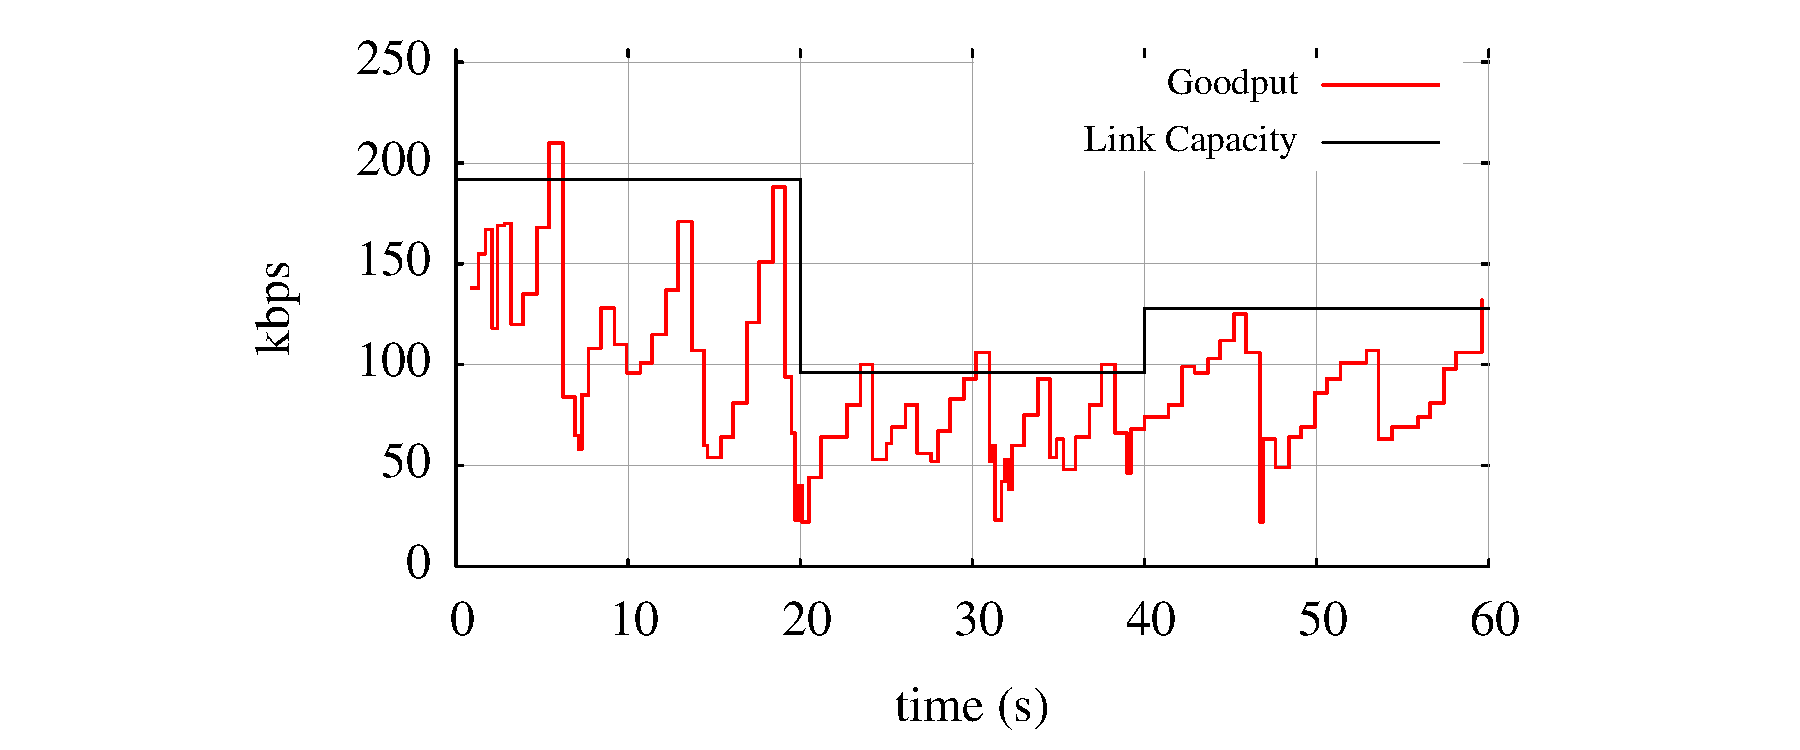
\includegraphics[width=0.5\textwidth, clip=true, trim=3cm 0 4.5cm 0]
      {chap5_graph_sl_cnadu}
    }
    \subfloat[C-NADU]{
      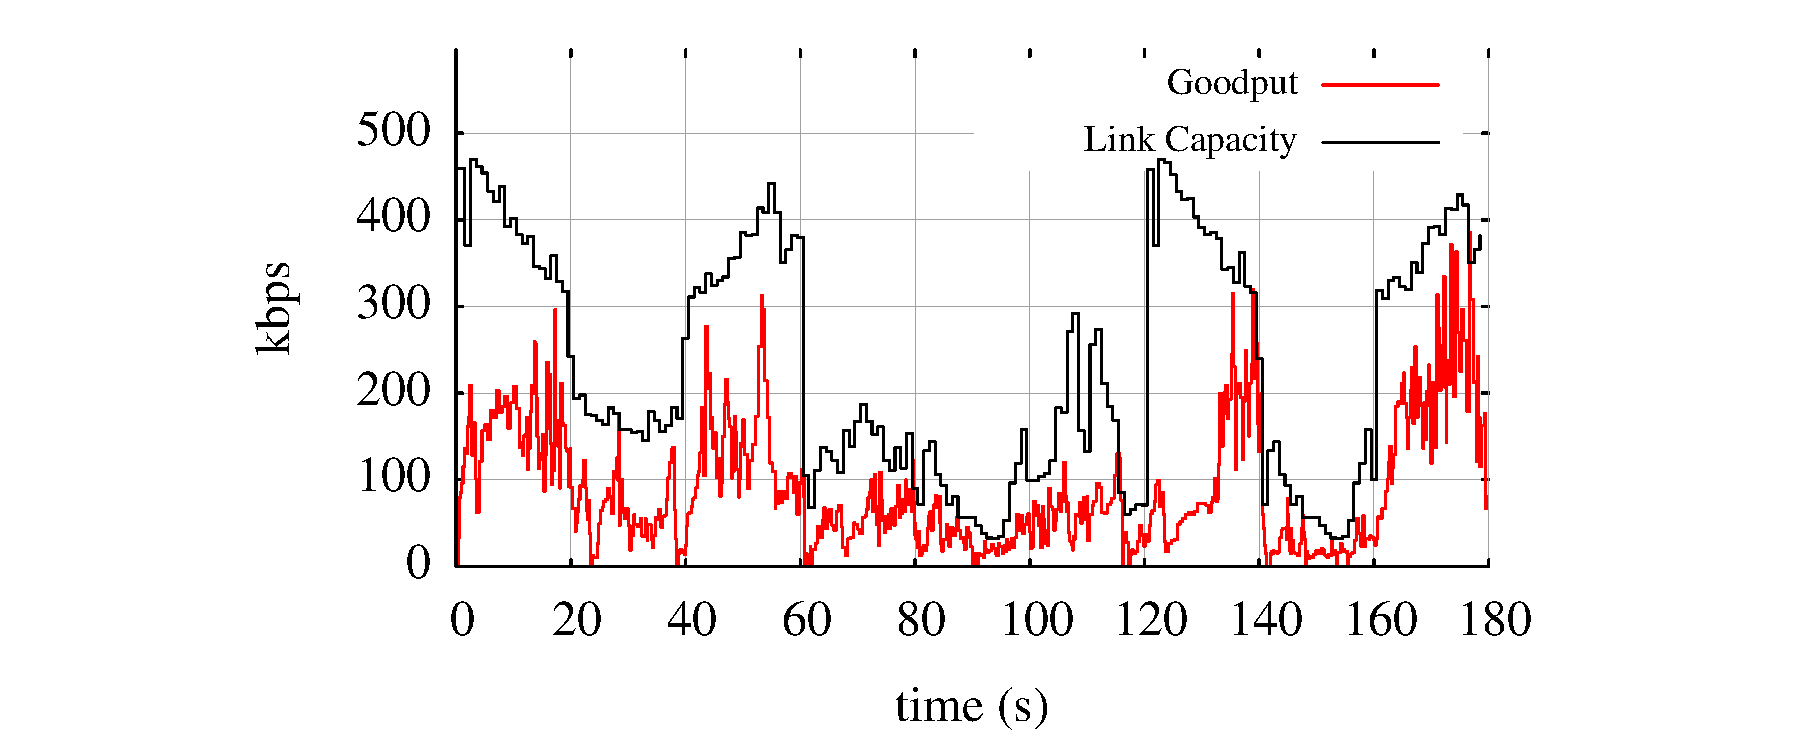
\includegraphics[width=0.5\textwidth, clip=true, trim=3cm 0 4.5cm 0]
      {chap5_graph_3g_cnadu}
    }
  }
  \caption{TPerformance of TFRC, TMMBR and C-NADU in a slow
  time-varying link (a, c, e) and 3G network (b, d, f).}
  \label{fig:3grc}
\end{figure}


\begin{table}[!t]
\centering{
\begin{tabular}{cccc}
\hline
 & $Goodput_{avg}$ & PLR & $PSNR_{avg}$\\
 & (kbps)  &(\%) & (dB)\\
\hline
TFRC & 84.1 & 6.9\,\%& 29.3 \\ %
TMMBR & 89.8 & 3.7\,\% & 30.5 \\ %
%NADU & 106 & 93 & 29.9& 6.3\%\\%
C-NADU & 92 & 2.2\,\% & 31.9 \\%
\hline
\end{tabular}
}
\caption{Comparing TFRC, TMMBR, C-NADU for calls over mobile nodes (180\,\emph{s}
simulations using 3G traces).}
\label{table:3grc}
\end{table}

\section{Performance Analysis of TFRC, TMMBR, C-NADU, and RRTCC}

This section briefly discusses the performance of each congestion control
algorithm. The detailed analysis can be found in the respective papers.

Our results in \citepub{c:3grc} show that TFRC produces a sawtooth sending
rate, similar to the performance in~\cite{saurin:2006:thesis}. When the media
stream is the only flow on the end-to-end path, we also observe that the average
bandwidth utilization (ABU) is between 30-40\,\%, i.e., TFRC under utilizes the
link and the loss ratio is about 6\,\%, which results in a lower media quality
(approximated by measuring PSNR) compared with the other two schemes (see
Table~\ref{table:3grc}). TMMBR-based congestion control utilizes the link
better than TFRC (ABU between 50-70\,\%) and produces a lower loss ratio
($\approx$3\,\%). Lastly, C-NADU has comparable bandwidth utilization
(ABU=55-60\,\%) and loss ratio ($\approx$2\,\%) to TMMBR.
Figure~\ref{fig:3grc} shows the performance of TFRC, TMMBR and C-NADU over two
types of bottleneck links, a slow time-varying link and a 3G link.


\begin{figure}[!t]
\centerline{
%\hfill
\subfloat [Call 1 vs Call 2] {\label{fig_sim-mixed-1-1}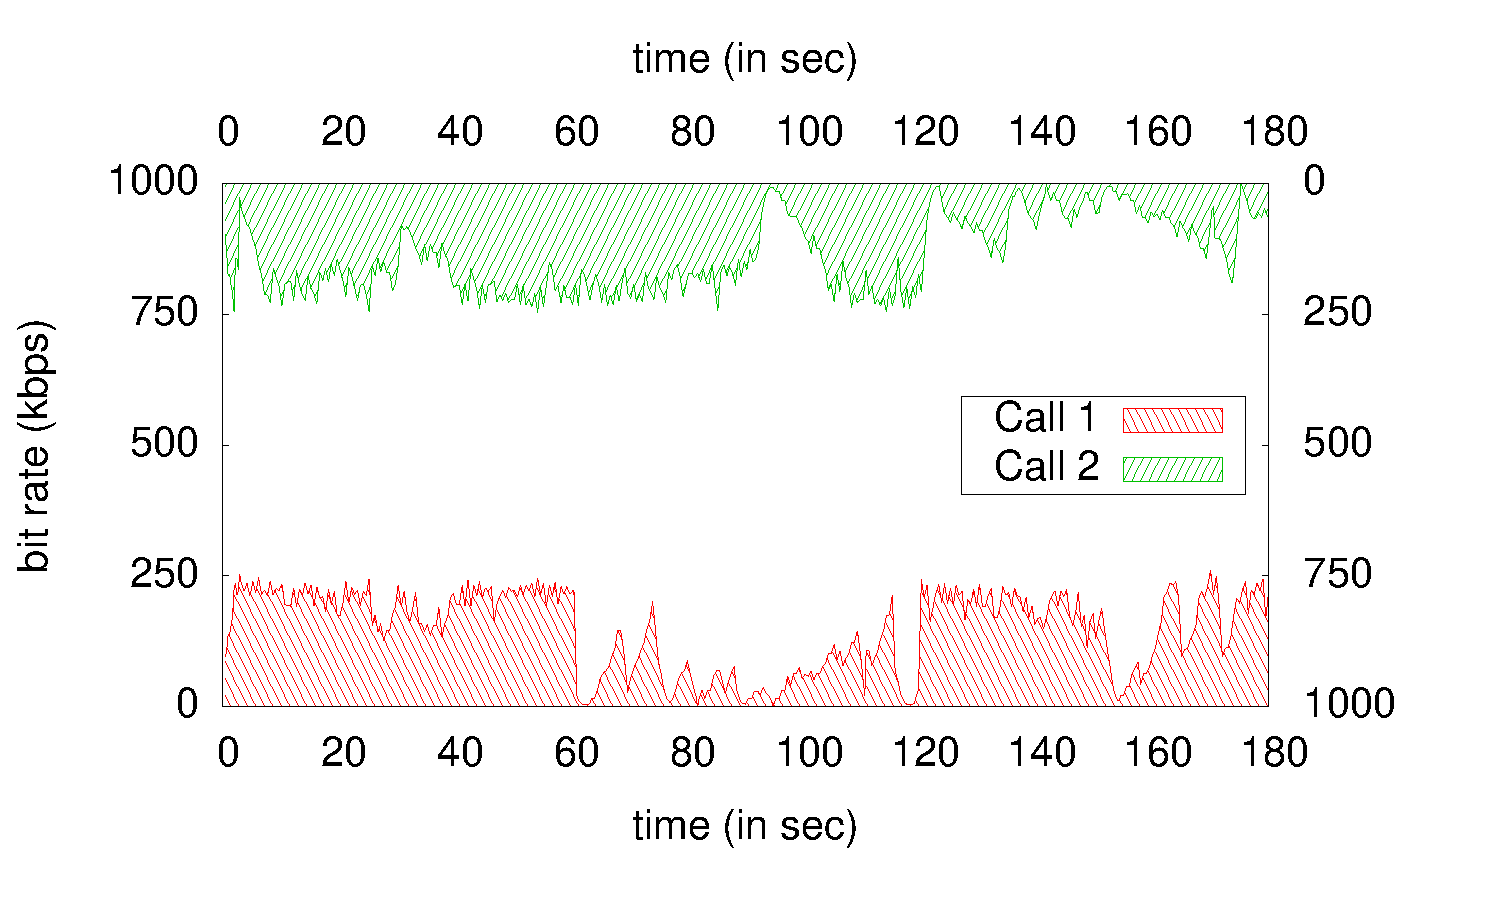
\includegraphics[width=0.5\textwidth]{chap5-graph-5rtp_uc1_12}%
}
%\hfill
\subfloat [Call 1 vs Call 3] {\label{fig_sim-mixed-1-2}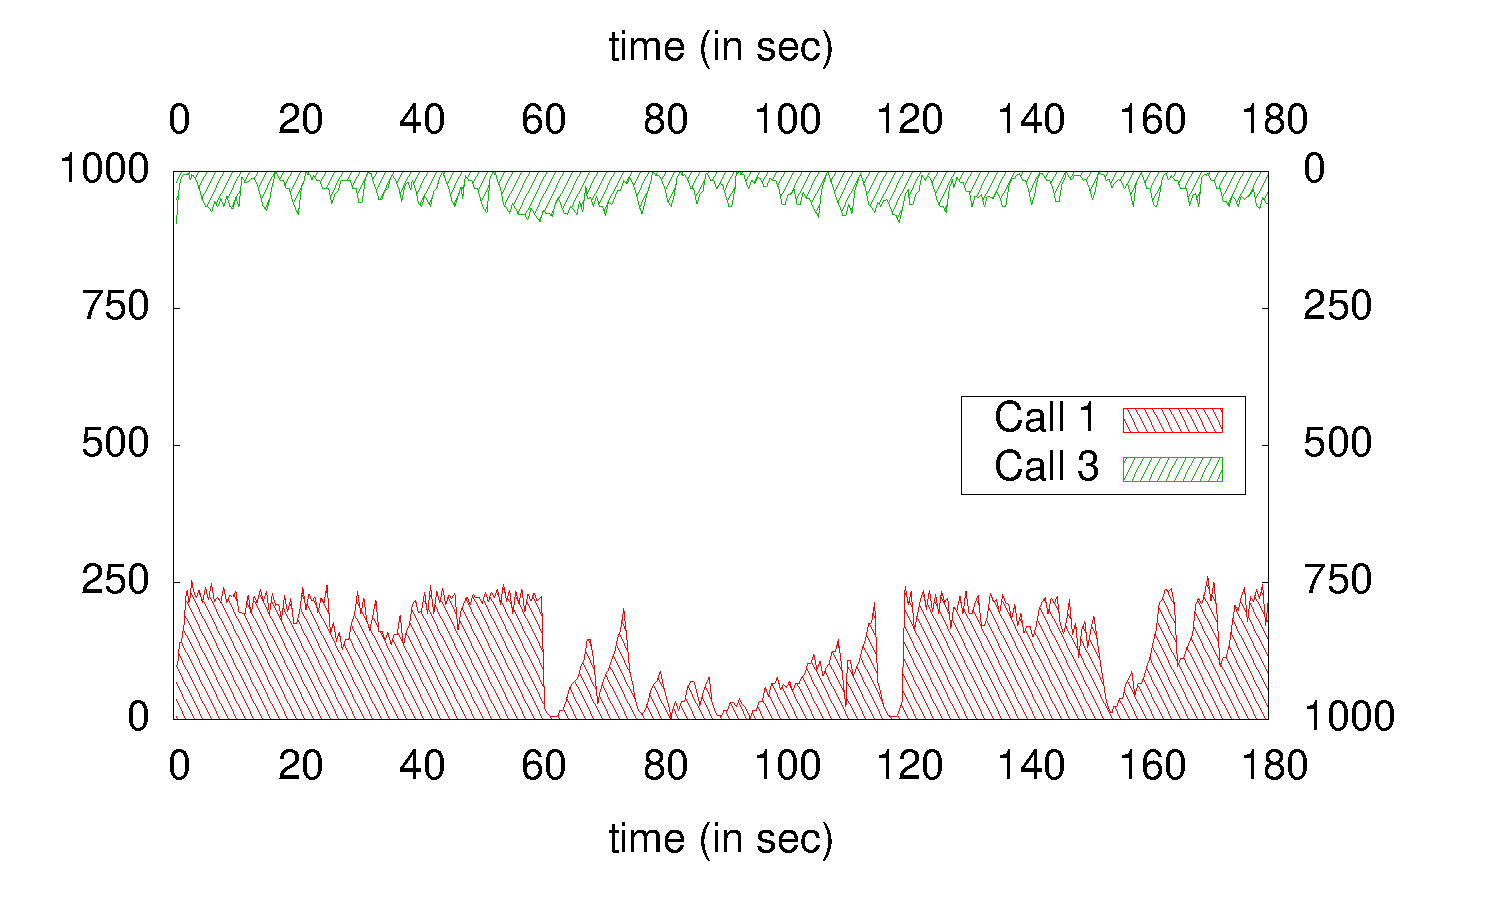
\includegraphics[width=0.5\textwidth]{chap5-graph-5rtp_uc1_13}%
}
%\hfill
}
\centerline{
%\hfill
\subfloat [Call 1 vs Call 4] {\label{fig_sim-mixed-1-3}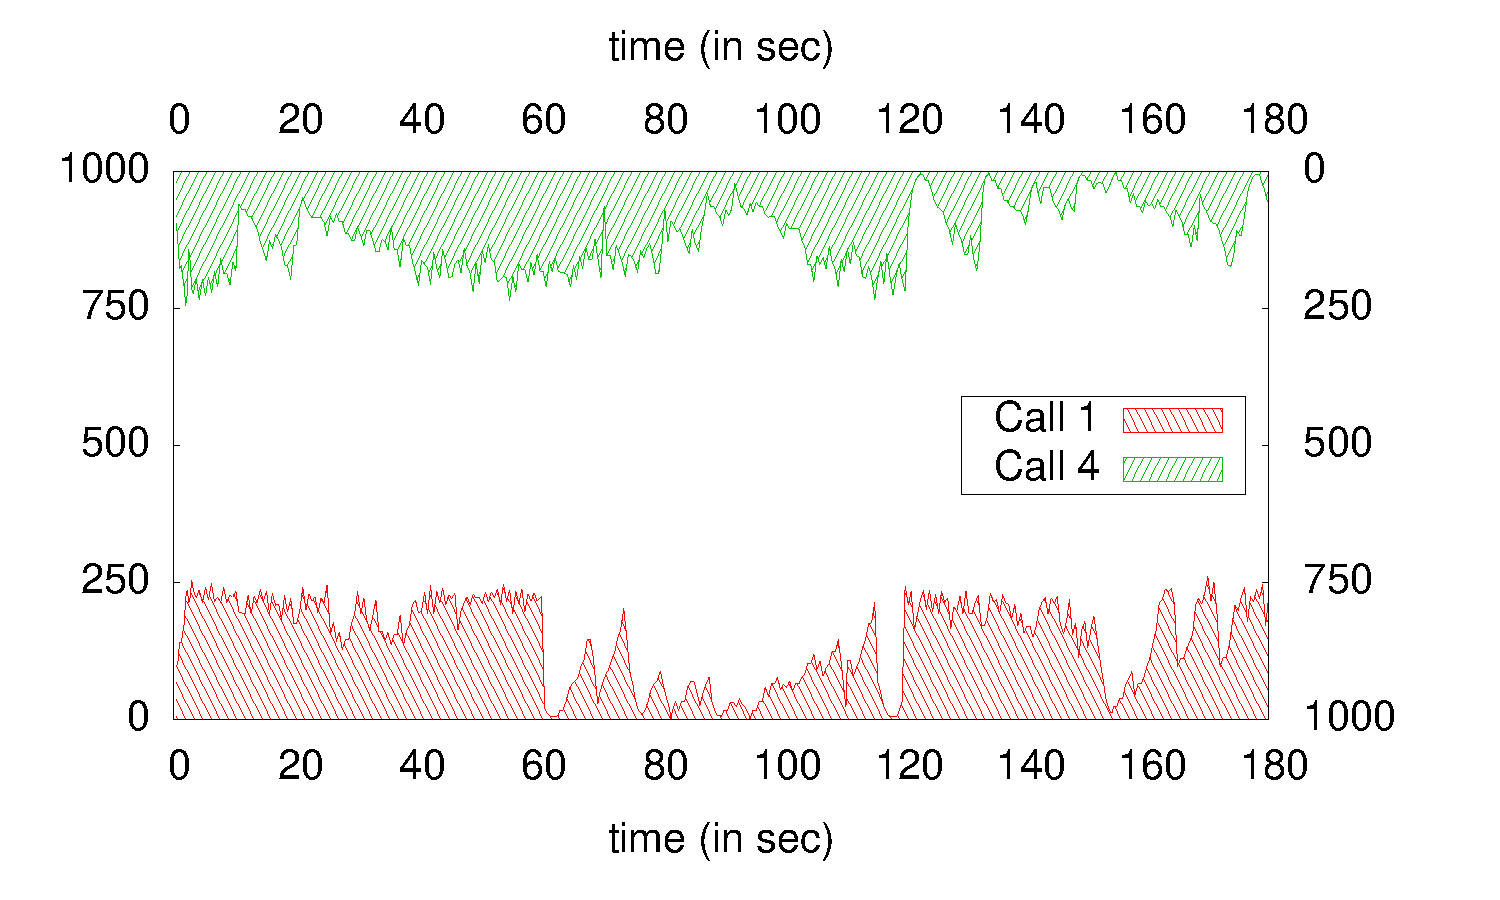
\includegraphics[width=0.5\textwidth]{chap5-graph-5rtp_uc1_14}%
}
%\hfill
\subfloat [Call 1 vs Call 5] {\label{fig_sim-mixed-1-4}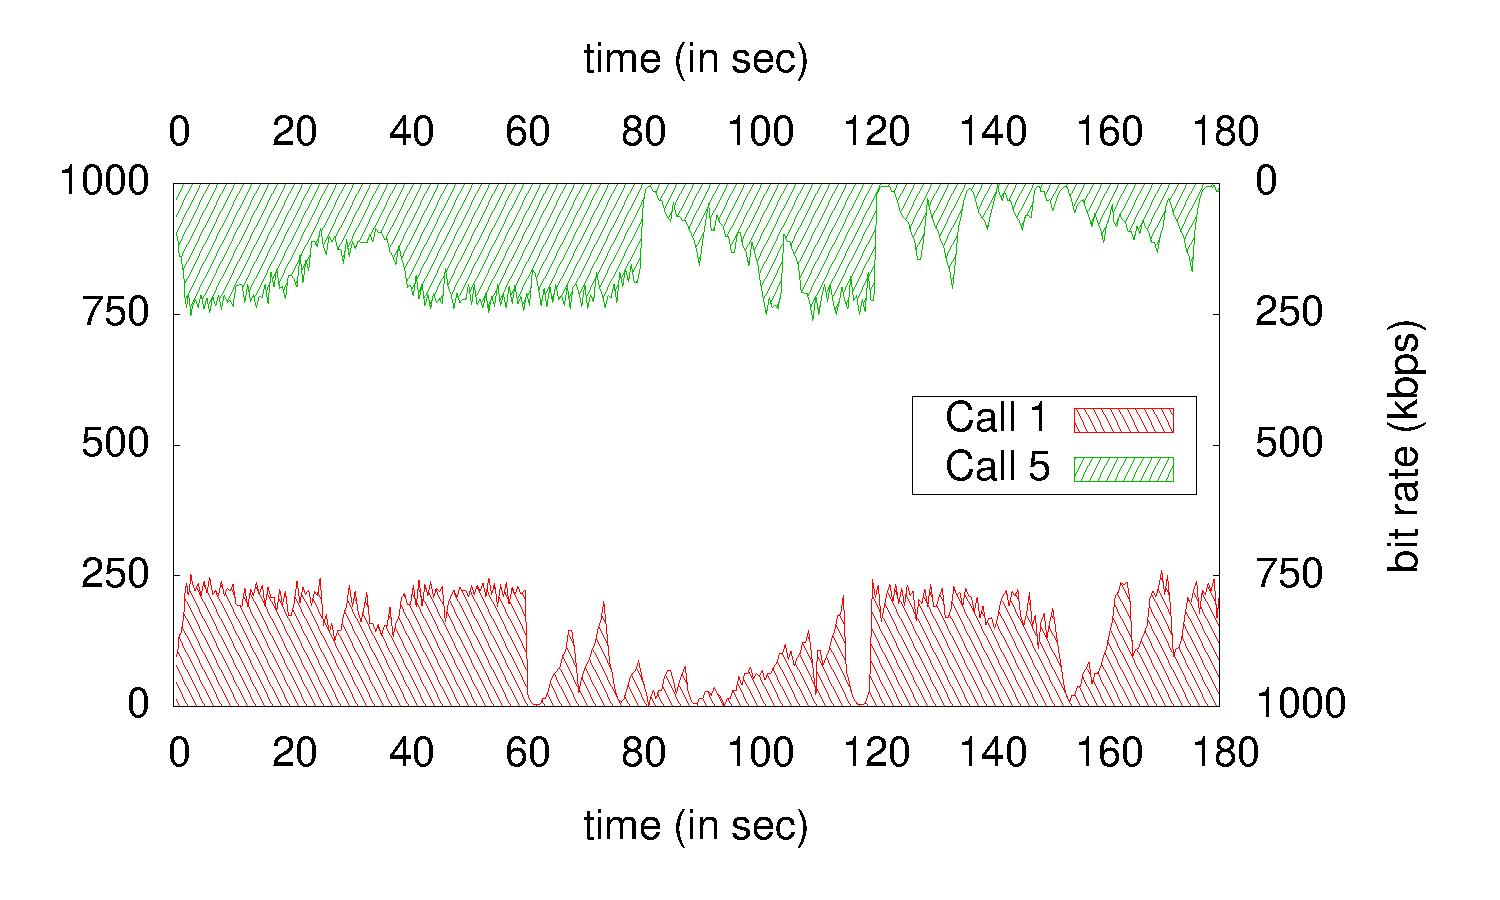
\includegraphics[width=0.5\textwidth]{chap5-graph-5rtp_uc1_15}%
}
%\hfill
}
\caption{Performance of five C-NADU calls competing for
capacity on a shared bottleneck in a heterogeneous network. Each call needs
to quickly adapt to changes in 3G link capacity and fairly share the
bottleneck link.}
\label{fig:hetrc}
\end{figure}

\begin{table}[!t]
\centering{
\scalebox{0.9}{
\begin{tabular}{cccccc}
\hline
 & 3G Capacity & $Goodput_{avg}$ & PLR & $PSNR_{avg}$ & ABU \\
 & Pattern & (kbps) & (\%) & (dB) ($\sigma$)  & (\%) \\ 
\hline
Call 1 & Excellent-Poor-Elevator & 140.10 & 2.15\,\% & 31.4 ($0.39$) & 70.1\,\% \\ 
Call 2 & Good-Good-Poor & 133.55 & 1.61\,\% & 31.9 ($0.62$)& 66.8\,\% \\ 
Call 3 & Poor-Poor-Poor & 35.18 & 1.55\,\% & 22.2 ($1.13$)& 17.59\,\% \\ 
Call 4 & Fair-Fair-Poor & 114.96 & 2.75\,\% & 31.1 ($0.75$)& 57.5\,\% \\ 
Call 5 & Excellent-Elevator-Poor & 130.23 & 2.25\,\% & 31.3 ($0.13$)& 65.1\,\% \\ 
\hline
\end{tabular}
}}
\caption{C-NADU: Five calls in a heterogeneous network with end-to-end latency
between 60-120\,\emph{ms} and 0.5\,\% link-layer losses.}
\label{table:hetrc}
\end{table}

In \citepub{c:hetrc}, we show that C-NADU is self-fair with other C-NADU flows
in both wired and wireless environments~\cite{singh:2010.thesis}, and in
\citepub{c:fecrc} we show that it competes fairly with TCP cross-traffic, for both
the long- and short-TCP flows. Figure~\ref{fig:hetrc} show five video calls in which
each sender uses an independent 3G link into a common bottleneck to the
receivers. The 3G links are based on radio link traces and have different
capacities. Hence, at some instances of time, the 3G link is the constraint and
at other times it is the shared bottleneck link. Table~\ref{table:hetrc} shows that
four calls have comparable performance (see PSNR and goodput) and one call suffers
due to poor connectivity (the 3G link has insufficient capacity which affects
the quality).

\begin{figure}[!t]
  \centerline{
    \subfloat{
      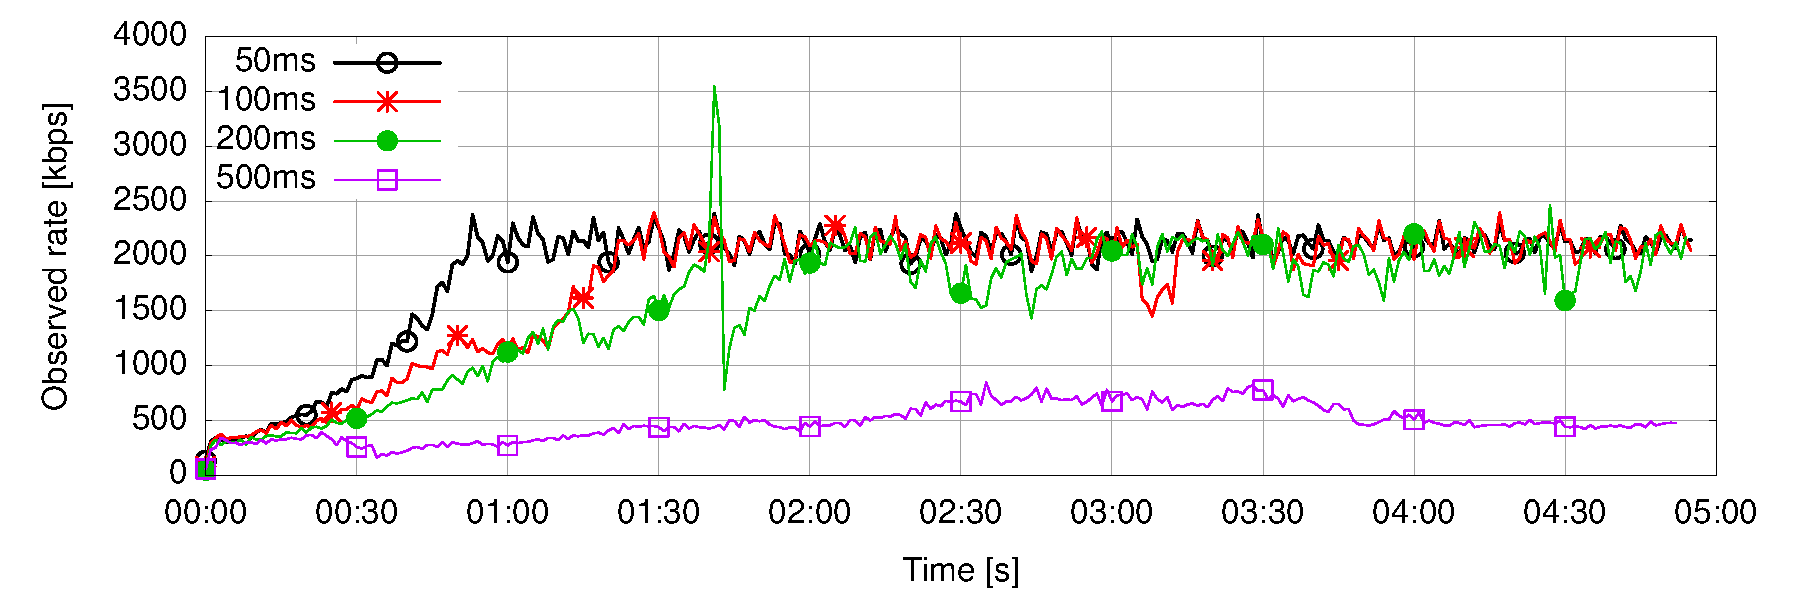
\includegraphics[width=0.8\textwidth]
      {chap5-graph-rrtcc-latency}
    }
   }
   \centerline{
    \subfloat{
      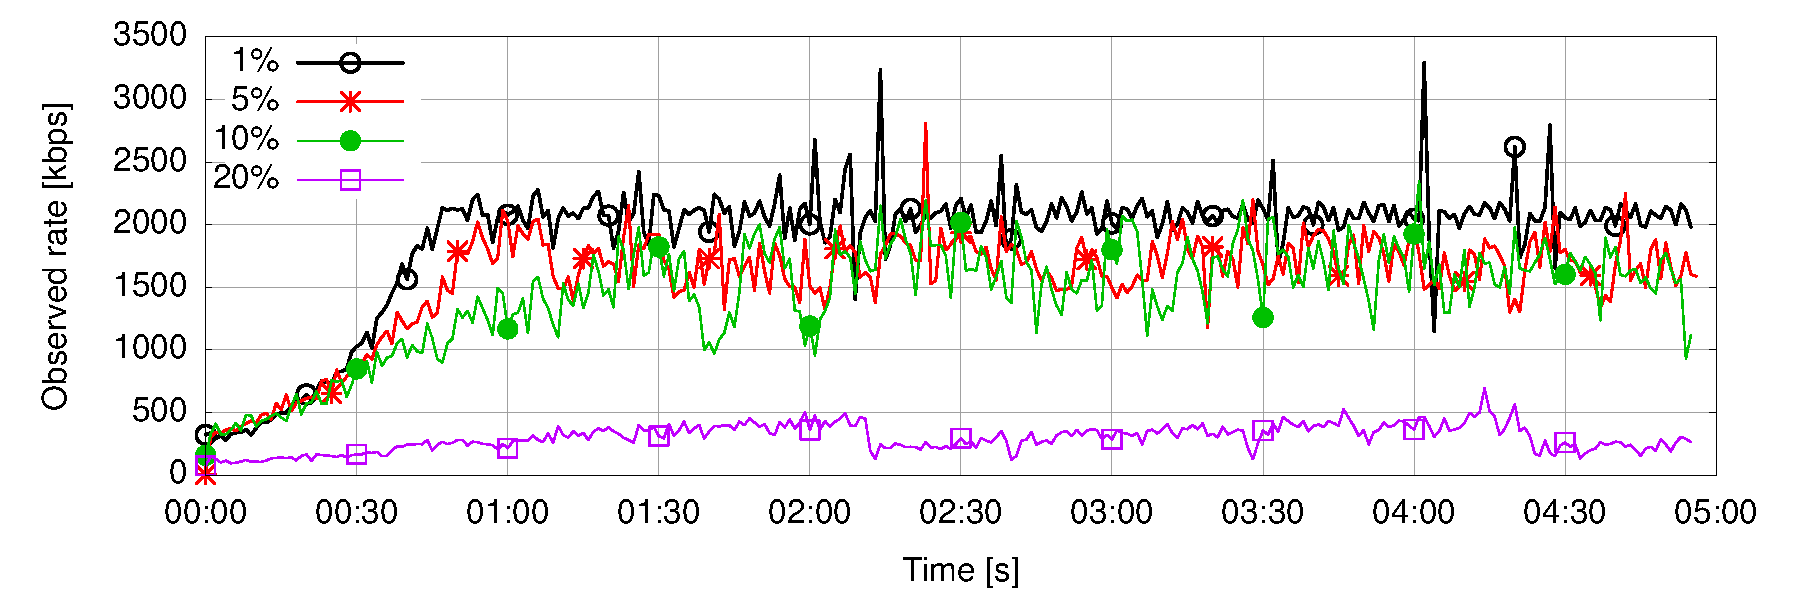
\includegraphics[width=0.8\textwidth]
      {chap5-graph-rrtcc-plr}
    }
  }
  \caption{The plots show the performance of RRTCC on a link with varying
  delay and fractional loss rate. We observe that by the sending rate
  decreases with increasing link latency or bit-error loss. }
  \label{fig:rrtcc-single}
\end{figure}

\begin{table}[!t]
\begin{center}{
  \scalebox{0.9}{
\begin{tabular}{ ccccc }
\hline
 & $Goodput_{avg}$ & Residual  & PLR\\
 & (kbps)  & Loss (\%) & (\%)\\
\hline
 0\,\% & 1949.7 $\pm$ 233.62 & 0.011 & 0.011 \\ 
 5\,\% & 1568.74 $\pm$ 178.52 & 0.23 & 9.77 \\ 
 10\,\% & 1140.82 $\pm$ 161.92 & 0.49 & 19.02 \\ 
 20\,\% & 314.4 $\pm$ 61.98 & 2.43 & 36.01 \\ \hline
\end{tabular}
}}
\end{center}
\caption{RRTCC: Metrics for a bottleneck with different packet loss rates.}
\label{tab:rrtcc-loss}
\end{table}

In \citepub{c:eval}, we evaluate the performance of RRTCC in several
scenarios: by itself on a bottleneck link, competing with other RRTCC flows
and competing with TCP cross-traffic. Figure~\ref{fig:rrtcc-single} shows an
example plot of the performance of RRTCC. In Figure~\ref{fig:rrtcc-single}(a) when
increasing the bottleneck link latency reduces the sending rate of RRTCC.
Similarly, Figure~\ref{fig:rrtcc-single}(b) shows that when increasing the loss
rate also affects the sending rate. However, Table~\ref{tab:rrtcc-loss} shows
that even though the link has a high loss rate, the residual loss rate is low
(even when the loss was 20\,\%), mainly due to the use of NACKs, PLI and FEC.


\begin{figure}[!t]
\centerline{
  \subfloat[Start together]
    {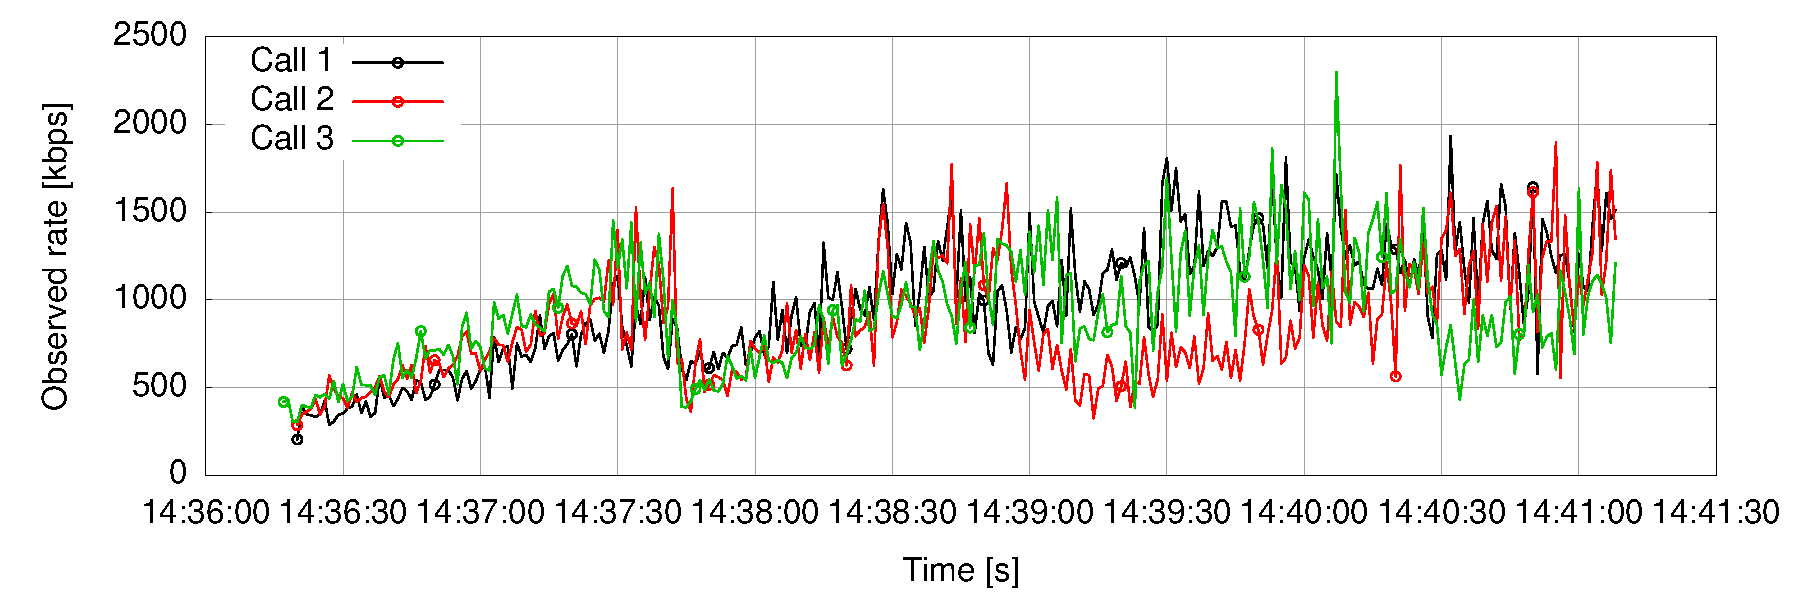
\includegraphics[width=0.8\textwidth]
    {chap5-graph-rrtcc-three-calls-sync}}
  }
  \centerline{
  \subfloat[Start 30\,\emph{s} apart]
    {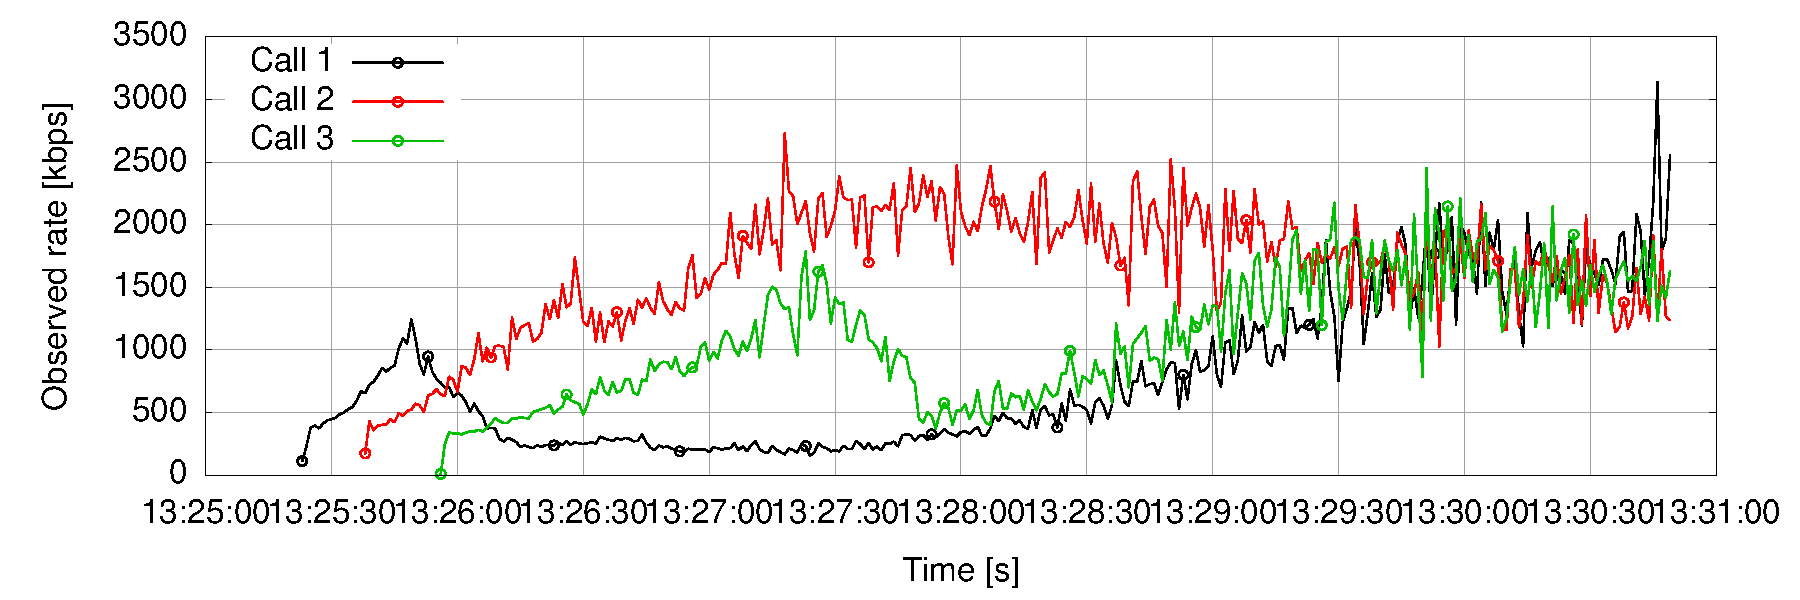
\includegraphics[width=0.8\textwidth]
    {chap5-graph-rrtcc-three-calls-async}}
  }
   \caption{The plots show the variation in receiver rate of three RRTCC
   flows, a) starting together, b) starting 30\,\emph{s} apart. The total duration of
   the call is 5 mins (300\,\emph{s}).}
\label{fig:rrtcc-self-fair}
\end{figure}

\begin{table}[!t]
\begin{center}
  \scalebox{0.9}{
\begin{tabular}{ccccc}
\hline
& $Goodput_{avg}$  & RTT & Residual & PLR\\
& (kbps)& (ms) & Loss (\%) & (\%)\\ \hline
 3 calls &  809.07 $\pm$ 202.38 &   31.48 $\pm$ 24.93 & 0.21 & 0.23 \\  
 3 calls (time shifted) &  1154.32 $\pm$ 250.54 &   35.15 $\pm$ 27.88 & 0.08 & 0.91 \\ \hline
\end{tabular}
}
\end{center}
    \caption{RRTCC competing with similar cross-traffic on the bottleneck link.}
    \label{tab:self-fair}
\end{table}

Next, we emulate three calls sharing a common bottleneck. In this case, the
individual media rates do not reach their individual maximum rate of 2\,\emph{Mbps}.
Figure~\ref{fig:rrtcc-self-fair}(a) shows that the three calls ramp up at about the
same rate, reach a peak and drop their rate simultaneously. The sending rates
synchronize, even though the flows originate from different endpoints using
independent RTP stacks.

Lastly, instead of the three calls starting together, each call starts at 30\,\emph{s}
intervals. We observe that while the media rate per call on average is higher,
the first call has a disadvantage. In all the cases, the first media flow temporarily 
starves when a new flow appears, ramping up again after a few minutes.
Figure~\ref{fig:rrtcc-self-fair}(b) shows the instantaneous rates of each of
the calls. The first call temporarily starves when new flows appear because,
when it starts, it is the only flow on the bottleneck and does not encounter
any queues; it observes a certain RTT and uses that as the baseline. When the
second flow appears, the second flow already observes queues from the existing
stream and competes with it, while the initial flow observes an increase in
queues and reduces the sending rate to avoid congestion.


To summarize, we observe that the performance of TFRC is bursty, which may
lead to poor user-experience, whilst TMMBR, C-NADU and RRTCC have a more
stable throughput. Lastly, TMMBR appears to be conservative with very low
packet loss, while RRTCC appears to be aggressive with a lot more packet loss.
C-NADU appears to be in between the two schemes, with higher throughput than
TMMBR and much lower packet loss compared to RRTCC. 

\section{Summary}

In this chapter, we describe congestion control implemented using congestion
cues from in-band sources and signaled in path (in RTCP). We further
categorize the congestion control algorithms based on \emph{where they are
implemented}: sender-driven scheme (e.g., TFRC), receiver-driven scheme (e.g.,
TMMBR), or co-operative scheme (combination of sender and receiver, e.g.,
C-NADU, RRTCC) and compare the performance of algorithms in each scheme. Our
initial experiments show that that C-NADU or TMMBR would be preferred, but
requires further investigation with more complex aggregate flows (mainly short
or bursty TCP flows).

In the next chapter, we discuss the interaction between the error-resilience
algorithm and the congestion control algorithm and evaluate if FEC can be used
as a probing mechanism by a multimedia congestion control algorithm.

%% An example for changing the running header (the optional parameter)

\chapter{Interaction of Error-Resilience and Congestion Control}
\label{chap:er-cc}

\chapter{Multihoming, Offloading, Overlays and Mobility}
\label{chap:mprtp}

\chapter{Network-assisted Congestion Control}
\label{chap:cc.nw}

\chapter{Conclusions}
\label{chap:conc}

%% The following commands are for article dissertations, remove them if you write a monograph dissertation.

% Errata list, if you have errors in the publications.
%\errata

%% The first publication (journal article)
% Set the publication information.
% This command musts to be the first!
\addpublication[conference]{Devadoss J., Singh V., Liu C., Ott J., Wang Y-K., Curcio I.}{Evaluation of Error Resilience Mechanisms for 3G Conversational Video}{IEEE ISM}{Berkley, USA}{Dec}{2008}{IEEE}{c:err}
% Add the dissertation author's contribution to that publication (the order can be interchanged with \adderrata).
\addcontribution{The author of this dissertation was one of the co-authors of the paper~\cite{Devadoss:3gErr}. His
contribution consisted of providing 2 out of the 4 ideas discussed in the paper, 
implementing the corresponding algorithms, providing the configurations for the experiments 
and co-editing the paper.}
% Add the errata of the publication, remove if there are none (the order can be interchanged with \addauthorscontribution).
%\adderrata{This is wrong}
% Add the publication pdf file, the filename is the parameter (must be the last).
%\addpublicationpdf{add/1_3g_er.pdf}

\addpublication[submitted]{V. Singh, J. Ott, C. Perkins}{Circuit Breakers}{---}{}{}{2013}{}{c:cb}
% Add the dissertation author's contribution to that publication.
\addcontribution{The author of this dissertation was the main author of this paper. 
His contribution consisted of implementing the algorithms and analyzing the results. He also 
acted as the main editor of the paper.}
% Add the errata of the publication, remove if there are none. (in submitted paper this is unlikely)
%\adderrata{This is wrong}
% Add the publication pdf file, the filename is the parameter.
%\addpublicationpdf{add/}

%% The second publication (conference article, note the optional parameter)
% Set the publication information.
\addpublication[conference]{V.Singh, J. Ott, I. D. D. Curcio}{Rate adaptation for 3G Conversational Video}{IEEE Infocom Workshops}{Rio de Janeiro, Brazil}{04}{2009}{IEEE}{c:3grc}
% Add the dissertation author's contribution to that publication.
\addcontribution{The author of this dissertation was the main author of the paper~\cite{Singh:3gRC}. His
contribution consisted of implementing the system and analyzing the results.}
% No errata
% Add the publication pdf file, the filename is the parameter.
%\addpublicationpdf{add/2_3g_ra.pdf}

%% The third publication (another journal paper, accepted for publication, note the optional parameter)
% Set the publication information, detailed information can be empty
\addpublication[conference]{V. Singh, J. Ott, I. D. D. Curcio}{Rate Adaption for Conversational Video in Heterogeneous Environments}{IEEE World of Wireless, Mobile and Multimedia (WoWMoM)}{San Francisco, USA}{06}{2012}{IEEE}{c:hetrc}
% Add the dissertation author's contribution to that publication.
\addcontribution{The author of this dissertation was the main author of the paper~\cite{Singh:HetRC}. His
contribution consisted of implementing the system and analyzing the results.}
% Add the errata of the publication, remove if there are none.
%\adderrata{This is wrong}
% Add the publication pdf file, the filename is the parameter.
%\addpublicationpdf{add/3_het_ra.pdf}

\addpublication[submitted]{M. Nagy, V. Singh, J. Ott, L. Eggert}{Rate-control using FEC for Interactive Multimedia Communication}{---}{}{}{2013}{}{c:fecrc}
% Add the dissertation author's contribution to that publication.
\addcontribution{The author of this dissertation was one of the co-authors of the paper. His
contribution consisted of providing the main idea for the paper, implementing the comparative 
algorithms, providing the configurations for the experiments and co-editing the paper.}

% Add the errata of the publication, remove if there are none. (in submitted paper this is unlikely)
%\adderrata{This is wrong}
% Add the publication pdf file, the filename is the parameter.
%\addpublicationpdf{add/6_fec_ra.pdf}

%% The fourth publication (yet another journal paper, submitted for publication, note the optional parameter)
%% Note that you are allowed to use this option only when submitting the dissertation for pre-examination!
% Set the publication information, detailed information is not printed
\addpublication[conference]{V. Singh, J. Ott, I. D. D. Curcio}{Predictive Buffering for Streaming Video in 3G Networks}{IEEE World of Wireless, Mobile and Multimedia (WoWMoM)}{San Francisco, USA}{06}{2012}{IEEE}{c:glass}
% Add the dissertation author's contribution to that publication.
\addcontribution{The author of this dissertation was the main author of the paper~\cite{Singh:Glass}. His
contribution consisted of implementing the system and analyzing the results.}
% Add the errata of the publication, remove if there are none. (in submitted paper this is unlikely)
%\adderrata{This is wrong}
% Add the publication pdf file, the filename is the parameter.
%\addpublicationpdf{add/4_glass.pdf}

\addpublication[conference]{V. Singh, S. Ahsan, J. Ott}{MPRTP: Multipath Considerations for Real-time Media}{ACM Multimedia Systems (MMSys)}{Oslo, Norway}{02}{2013}{ACM}{c:mprtp}
% Add the dissertation author's contribution to that publication.
\addcontribution{The author of this dissertation was the main author of the paper~\cite{Singh:MPRTP}.
His contribution consisted of providing the main idea for the paper, providing
the configurations for the experiments, performing the statistical analysis, 
and acting as the main editor of the paper.}
% Add the errata of the publication, remove if there are none. (in submitted paper this is unlikely)
%\adderrata{This is wrong}
% Add the publication pdf file, the filename is the parameter.
%\addpublicationpdf{add/5_mprtp.pdf}

%\bibliographystyle{IEEEtran} %plain, 
\bibliographystyle{amsalpha}
% argument is your BibTeX string definitions and bibliography database(s)
%\bibliography{IEEEabrv,../allpapers}
\bibliography{bib/diss,bib/rfc}

\end{document}
